%% 
%% Copyright 2007, 2008, 2009 Elsevier Ltd
%% 
%% This file is part of the 'Elsarticle Bundle'.
%% ---------------------------------------------
%% 
%% It may be distributed under the conditions of the LaTeX Project Public
%% License, either version 1.2 of this license or (at your option) any
%% later version.  The latest version of this license is in
%%    http://www.latex-project.org/lppl.txt
%% and version 1.2 or later is part of all distributions of LaTeX
%% version 1999/12/01 or later.
%% 
%% The list of all files belonging to the 'Elsarticle Bundle' is
%% given in the file `manifest.txt'.
%% 

%% Template article for Elsevier's document class `elsarticle'
%% with numbered style bibliographic references
%% SP 2008/03/01

\documentclass[final,5p,twocolumn]{elsarticle}

%% Use the option review to obtain double line spacing
%% \documentclass[authoryear,preprint,review,12pt]{elsarticle}

%% Use the options 1p,twocolumn; 3p; 3p,twocolumn; 5p; or 5p,twocolumn
%% for a journal layout:
%% \documentclass[final,1p,times]{elsarticle}
%% \documentclass[final,1p,times,twocolumn]{elsarticle}
%% \documentclass[final,3p,times]{elsarticle}
%% \documentclass[final,3p,times,twocolumn]{elsarticle}
%% \documentclass[final,5p,times]{elsarticle}
%% \documentclass[final,5p,times,twocolumn]{elsarticle}

%% For including figures, graphicx.sty has been loaded in
%% elsarticle.cls. If you prefer to use the old commands
%% please give \usepackage{epsfig}

%% The amssymb package provides various useful mathematical symbols
\usepackage{amssymb}
\usepackage{xspace}
\usepackage{verbatim}
\usepackage[usenames]{color}
\usepackage[usenames,dvipsnames,table]{xcolor}
\usepackage{url}
\usepackage{array}
\usepackage{color}
\usepackage{longtable}
\usepackage{wrapfig}
\usepackage{tikz}
\usetikzlibrary{graphs}
\usetikzlibrary{backgrounds}
\usepackage{subcaption}

% \usepackage[pdftex,dvips]{graphicx}


%% The amsthm package provides extended theorem environments
%% \usepackage{amsthm}

%% The lineno packages adds line numbers. Start line numbering with
%% \begin{linenumbers}, end it with \end{linenumbers}. Or switch it on
%% for the whole article with \linenumbers.
%% \usepackage{lineno}

%% \journal{Nuclear Physics B}

\begin{document}

\begin{frontmatter}

%% Title, authors and addresses

%% use the tnoteref command within \title for footnotes;
%% use the tnotetext command for theassociated footnote;
%% use the fnref command within \author or \address for footnotes;
%% use the fntext command for theassociated footnote;
%% use the corref command within \author for corresponding author footnotes;
%% use the cortext command for theassociated footnote;
%% use the ead command for the email address,
%% and the form \ead[url] for the home page:
%% \title{Title\tnoteref{label1}}
%% \tnotetext[label1]{}
%% \author{Name\corref{cor1}\fnref{label2}}
%% \ead{email address}
%% \ead[url]{home page}
%% \fntext[label2]{}
%% \cortext[cor1]{}
%% \address{Address\fnref{label3}}
%% \fntext[label3]{}

\title{Whole-body multi-contact motion in Humans and Humanoids}

%% use optional labels to link authors explicitly to addresses:
%% \author[label1,label2]{}
%% \address[label1]{}
%% \address[label2]{}

\author{Vincent Padois}
\address{Sorbonne Universit�s, UPMC Univ. Paris 06 and CNRS Institut des Syst�mes Intelligents et de Robotique F-75005, Paris, France. Email: vincent.padois@upmc.fr }

\author{Serena Ivaldi}
\address{French Institute for Research in Computer Science and Automation (INRIA) Nancy Grand-Est, France. Email: serena.ivaldi@inria.fr}

\author{Jan Babic}
\address{Faculty of Electrical Engineering Josef Stefan Institute, Slovenia Email: jan.babic@ijs.si}

\author{Michael Mistry }
\address{University of Birmingham, UK Email: m.n.mistry@bham.ac.uk}

\author{Jan Peters}
\address{Max Planck Institute for Intelligent Systems and TU Darmstadt, Germany
Email: mail@jan-peters.net}

\author{Francesco Nori}
\address{Robotics, Brain and Cognitive Science Department Istituto Italiano di Tecnologia. Email: francesco.nori@iit.it}


\begin{abstract}
Traditional industrial applications involve robots with limited mobility. Consequently, interaction (e.g. manipulation) was treated separately from whole-body posture (e.g. balancing), assuming the robot firmly connected to the ground. Foreseen applications involve robots with augmented autonomy and physical mobility. Within this novel context, physical interaction influences stability and balance. To allow robots to surpass barriers between interaction and posture control, forthcoming robotic research needs to investigate the principles governing whole-body motion and coordination with contact dynamics. There is a need to investigate the principles of motion and coordination of physical interaction, including the aspects related to unpredictability. Recent developments in compliant actuation and touch sensing allow safe and robust physical interaction from unexpected contact including humans. The next advancement for cognitive robots, however, is the ability not only to cope with unpredictable contact, but also to exploit predictable contact in ways that will assist in goal achievement. Last but not least, theoretical results needs to be validated in real-world scenarios with humanoid robots engaged in whole-body goal-directed tasks. Robots should be capable of exploiting rigid supportive contacts, learning to compensate for compliant contacts, and utilising assistive physical interaction from humans.
\end{abstract}

\begin{keyword}
whole-body \sep control \sep free-floating \sep interaction \sep contacts \sep compliance.
%% keywords here, in the form: keyword  keyword

%% PACS codes here, in the form: \PACS code \sep code

%% MSC codes here, in the form: \MSC code \sep code
%% or \MSC[2008] code \sep code (2000 is the default)

\end{keyword}

\end{frontmatter}

%% \linenumbers

%% main text
\section{Introduction}
\label{sec:intro}

For cognitive agents, such as humanoid robots, to persist and act in natural human environments, contact and physical interaction become necessary and unavoidable. Everyday tasks involve making and breaking contact, among all areas of the body, whether the contacts are accidental disturbances or intentional support for dynamic movement. Critically, robots should be robust enough to cope with unpredictable contact, via safe control mechanisms and compliance.  Moreover, cognitive goal directed robots need the ability to exploit predictable contact, to aid in goal achievement, as well as learn dynamics of contact in order to generalise to novel tasks and domains.

Physical interaction has been studied in robotics, extensively under the umbrella of manipulation. For historical reasons, these studies have assumed a fixed-base as cur-rent industrial applications do not necessitate extended mobility. Foreseen robotic applications will demand an increasing level of autonomy, including physical mobility. These applications call for extending studies on interaction to cases where the robot has a mobile-base. Remarkably and differently from the fixed-base case, inter-action in these situations may compromise system balance, and goal directed actions require proper whole-body coordination and use of contact. However, the principles governing whole-body coordination in humans are far from being understood and implementations on complex systems, such as humanoids, are missing, especially besides walking.

Within this context one of the major challenges of robotic research is to advance the current control and cognitive understanding about robust, goal-directed whole-body motion execution with multiple contacts. Remarkably, focus should be posed on complex systems, such as humans and humanoids. In a crescendo of complexity, as illustrated in the following figure, current state of the art (state-of-art 1 and 2) should be advanced to address more complex scenarios (challenges 1 and 2).
State-of-art 1: balancing with multiple rigid contacts. The robot is standing and balancing with its hands supported by a rigid table in front of its body. However, the table is too fragile, and unexpectedly breaks. A contact state change is sensed, and the robot's control architecture automatically adjusts posture control parameters to maintain balance in light of the reduced support. The unexpected breaking of contact makes it more challenging.

State-of-art 2: goal directed actions involving contacts. The robot is standing with its hands at its side, and intends to reach for an object on a table in front.  The robot recognises that the distance is sufficiently far away, and the task cannot be achieved without compromising balance.  The robot decides to initiate a new contact with its left hand on the table, providing sufficient support for reaching the object with its right hand.
Challenge 1: learning non-rigid contacts. The robot sits down on a chair with a soft cushion, however the cushion has a particular stiffness quality not experienced before. The robot tries to reach for an object on a table, but it fails as it did not adequately compensate for the unexpected dynamics of the soft cushion.  After a few attempts, the robot adapts its model of the contact interaction, and is able to infer new control action to successfully reach the goal.

Challenge 2: human assistive contacts. The robot is seated in a chair, and a per-son comes to assist the robot to stand. He/she grabs both hands of the robot and starts pulling upwards.  The robot senses the new contact, and recognising from the interaction force that it is an external agent, allows its arms to be compliant.  When the force becomes sufficient to enable standing, the robot recognises the intended action and stiffens its arms while pushing its legs to rise from the chair. Finally once standing, but still in contact with the human, the robot returns compliance to its arms to allow for safe interaction while retaining overall control of its posture.

\begin{figure}[!ht]
\centering
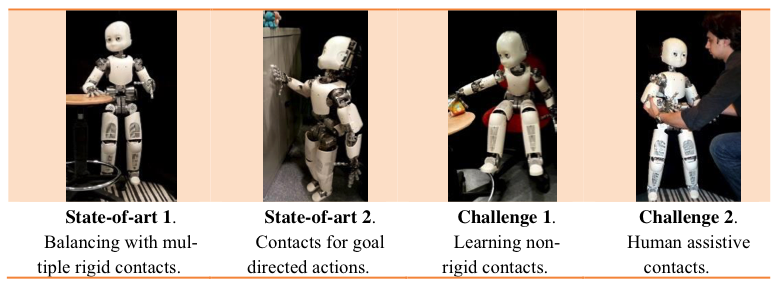
\includegraphics[width=0.7\linewidth]{./images/scenarios.png}
%\label{fig:subfig2}
\label{fig:scenarios}
\end{figure}

Present day robots are still far from the human capabilities in exploiting predictable events and in coping with uncertainty. The gap between humans and robots is particularly apparent when in tasks involving unstructured physical interaction with the environment or other agents. Recent behavioural experiments yielded a new perspective on modelling the way humans deal with both predictable and unpredictable motor control tasks. In early experiments, it has been shown \cite{Shadmehr1994a} that humans learn and adapt internal dynamical models of their own arm in interaction with the environment. Such internal models appear to be crucial in predicting how muscle activations pro-duce hand movements and therefore may play an essential predictive role in movement planning. However, Burdet et al. \cite{Burdet2001} have shown that when prediction is not a viable strategy, humans can rely on arm compliance regulation (by means of muscle co-activation) to cope with the unpredictability that naturally arises from feedback delays when performing arm-reaching movements in unstable environments. Basic research and robotics technology are ready to extend such insights from single limb movements to whole-body interaction and the validation of these models appears feasible. In contrast to manipulation scenarios with static base robot systems dynamic whole-body interaction concerns the analysis of phenomena at a higher scale (bigger interaction forces, bigger muscle activations, etc.). whole-body compliance regulation with force/impedance control is not only favoured by current theoretical progress and available technologies, but may actually be ready for wide-spread use instead of being limited to just a few prototypes.

\begin{figure}
\centering
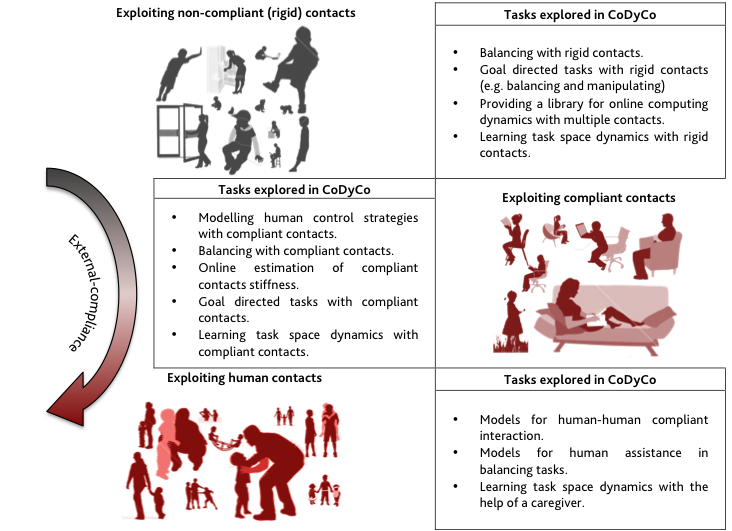
\includegraphics[width=\linewidth]{./images/classification1.png}
%\label{fig:subfig2}
\caption{Classification of whole-body tasks based on external-compliance. The complexity increases from top to bottom, i.e., with the need of exploiting the compliance of the contacts.}
\label{fig:classification1}
\end{figure}

\subsection{Roadmap beyond state-of-the-art}

With reference to Fig.~\ref{fig:classification1} and following, we propose a classification that relies on the well-known concept of compliance (or the inverse concept of stiffness), to be understood as the force-displacement characteristic of a contact. Interaction scenarios can be classified by quantitatively measuring two essential components of contacts: external and internal compliance (internal here refers to the agent or ``the self''). The first scenarios classification (Fig.~\ref{fig:classification1}) is based on the external-compliance; it includes scenarios that involve non-compliant (rigid) external contacts and scenarios with compliant external contacts. This second category is extremely wide in consideration of the multitude of possible compliant behaviours that can be experienced: from the linear force-displacement characteristic of a linear spring to the complex non-linear characteristic of a pillow. Scenarios within this category practically overlap with the first category but rigid contacts are replaced by non-rigid contacts. In these two categories the agent (or ``the self'', represented with a human silhouette) is always interacting with inanimate objects (the external contacts: a chair, a sofa, the floor, etc.). In the last category, ``the self'' and ``the other'' are both humans. In these scenarios the external-compliance is not a well-defined relationship between force and dis-placement but depends on the active intention of ``the other''.
External-compliance is only one side of the interaction, and the agent has limited control over it. The other side of the interaction is what we call the ``self'' (internal) compliance, which is instead fully under control of the cognitive agent. Self-compliance needs to be adapted to the environment compliance and the ability to actively regulate the internal compliance has been only recently implemented on multi-degrees-of-freedom robots. The self-compliance regulation represents the pro-active and cognitive component of the interaction and therefore gives the robot an enhanced degree of autonomy to be exploited in handling situations not anticipated at design time. In this sense, the self-compliance level and actuation range can be used to classify different scenarios as shown by Fig.~\ref{fig:classification2}. At the very first level of this classification we consider scenarios that do not require significant self-compliance regulation as they typically involve dynamically stable situations. Such situations involve for example dynamically stable tasks, which substantially require direct control of stable postures. The second level of the classification includes tasks that re-quire a certain level of active compliance either to stabilise unstable systems (e.g. balancing) or to compensate for unpredictable interaction characteristics (e.g. standing hand in hand with another agent). Finally at the highest level of this classification we consider highly complex tasks characterised by strong requirements in terms of ``self''-compliance planning and regulation.

\begin{figure}
\centering
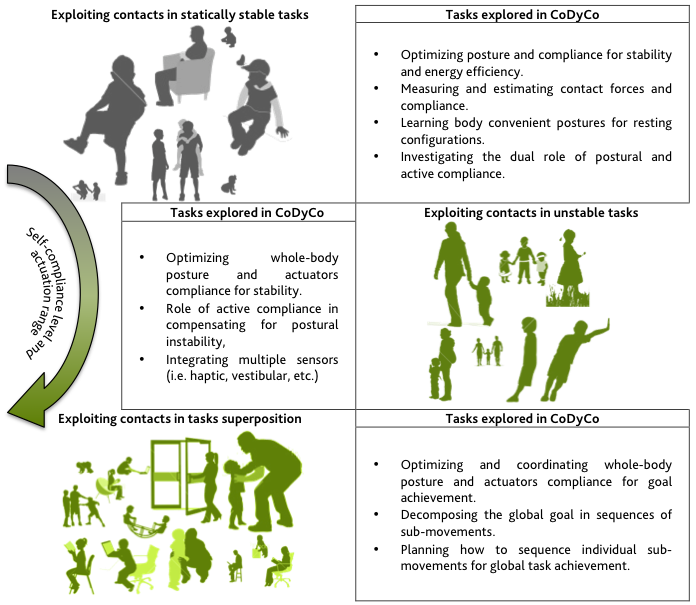
\includegraphics[width=\linewidth]{./images/classification2.png}
%\label{fig:subfig2}
\caption{Classification of whole-body tasks according to an increasing self-compliance level and actuation range.}
\label{fig:classification2}
\end{figure}

External and self-compliance are two fundamental aspects of any interaction. It is therefore crucial to understand how these two concepts become intertwined once con-tacts are established. We will introduce the concept of contact-compliance, which corresponds to the overall compliance obtained once the external and the self-compliance become coupled with the contact establishment. A contact can be seen as the serial connection of two compliances, one representing the external-compliance, the other representing the self-compliance. The compliance of a serial interconnection is simply the linear sum of the individual compliances. Roughly speaking, the con-tact-compliance does not significantly change when the external and self-compliance are changed simultaneously by an equal and opposite quantity. No advancement can be associated to situations which correspond to augmenting the self-compliance at the cost of diminishing the external-compliance or vice versa, as in these situations the overall contact-compliance does not change. This fundamental procedural principle is well sketched in Fig.~\ref{fig:classification3}. The horizontal axis sorts possible scenarios according to a progressively increasing external-compliance level. The vertical axis instead orders the same scenarios by means of increasing self-compliance levels and actuation ranges: tasks involving minimal self-compliance regulation or low levels of compliance are shown at the bottom; tasks involving wide self-compliance regulation ranges including high compliance levels are at the top. The grey-colour-valued function shown in the space defined by these two axes is a qualitative evaluation of progress beyond the state of the art: dark grey is the state-of-the-art, increasing levels of blue represent step-by-step progress beyond state of the art. Progress in handling whole body con-tacts can be achieved only by simultaneously increasing the external and the self-compliance levels. Conversely, little advances are achieved when increasing the environmental compliance but reducing the active compliance component. Vice versa, a dual way to achieve little progress beyond the state of the art corresponds to scenarios that involve a strong self-compliance regulation but reduced external compliance.  

\begin{figure}[!ht]
\centering
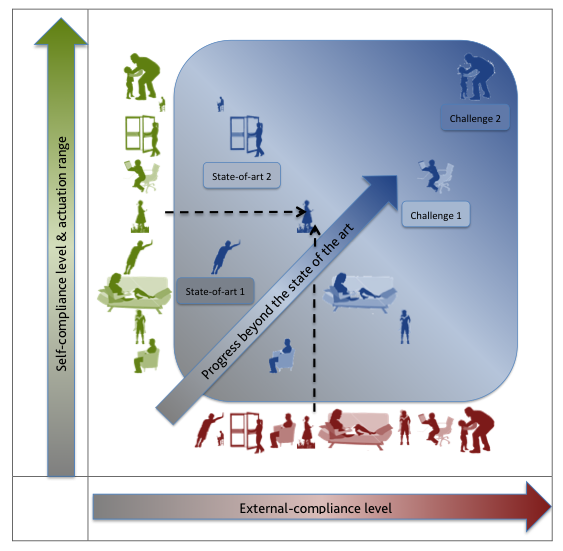
\includegraphics[width=\linewidth]{./images/classification3.png}
\caption{the metric space to evaluate the progress work beyond the current state-of-the-art. Interaction is the inter-twined combination of two components, external and self-compliance, both contributing to the concept of contact-compliance. Whole-body scenarios should be evaluated in a metric space that takes into account how self and external-compliance contribute to contact-compliance. Contact-compliance is the sum of self and external compliance. Remarkably the major advances can be obtained by simultaneously advancing the external and the self-compliance requirements. The vertical axis represents both self-compliance levels and actuation ranges in consideration of the fact we are mainly interested in self-compliance regulation, actuation and control. The four proposed scenarios have increasing complexity with respect to current state-of-the-art. }
\label{fig:classification3}
\end{figure}

\section{State-of-the-art}

Technological state of the art. Among the recent achievements in the field of robotics, there are two major technological prerequisites that will play a fundamental role in enhancing whole-body motion capabilities: distributed force and touch sensing. Both technologies have been only recently integrated and used in (humanoid) robots, including the iCub \cite{MettaG._etal2010}.
Force control is a fundamental property for any autonomous agent in interaction with the environment. First attempts to regulate interaction forces relied on active force and compliance control schemes, typically coupled with custom mechanical designs such as the ones proposed in \cite{Salisbury1988} and \cite{Hayashi2007} , which were eventually implemented on successful commercial manipulators. Similar solutions have been eventually implemented on some humanoid platforms \cite{Cheng2006} \cite{Escande2010}, including the iCub \cite{Fumagalli2012} . Recent theoretical and technological advances have revealed the importance of intentionally introducing mechanical compliance in the design \cite{Pratt1995} and (even more recently) the necessity of actively regulating the actuator passive compliance \cite{Koganezawa2005} \cite{Tonietti2005} \cite{Migliore2005} . It is to be expected that within the next years robots such as iCub will be equipped with variably compliant actuation technologies at some (if not all) of the main joints \cite{Tsagarakis2009} \cite{Tsagarakis2011} .
Touch is another fundamental sensing capability for autonomous agents willing to interact with an unstructured environment or humans \cite{Argall2010a} . Whole-body distributed touch sensing has been only recently embedded on humanoid robots, but there already exist quite a few examples: Robovie-IV \cite{Mitsunaga2006} , RI-MAN \cite{Mukai2008} , Macra \cite{Hayashi2007}  and Meka \cite{Jain} , just to cite a few. The iCub already integrates a mature technology \cite{Schmitz2011} cover-ing the upper body, legs and feet soles. 
Finally, several open-source software libraries have been developed in the last years to support research in whole-body dynamics and contact simulation. Several dynamics simulators have been developed for robotics (see \cite{ivaldi2014} for a survey). The most interesting physics engines for our purposes are the ones with Featherstone-like forward dynamics calculation \cite{Featherstone2008} \cite{Yamane2006a} , built-in collision detection and stable numerical contact forces computations \cite{Nakaoka2007} . Among the kinematic and dynamic libraries it is worth citing HuMAnS , a toolbox for analysis and control of both human and humanoid motion, and iDyn, a generic software tool, extensively used in iCub to compute whole-body dynamics and reinforce these computations with measurements coming from sensors embedded in the robot \cite{Fumagalli2012}.
Human motor control state-of-the-art. Human whole-body motion control has been studied within tasks such as reaching on a supporting surface and sit-to-stand. These movements involve coordination of multiple joints, significant shift of the centre of mass, and control of equilibrium, either in static or dynamic conditions. These are skills learnt early in human childhood but also studied extensively in the context of motor disability, e.g. after neurological insults like stroke, or in the elderly with reduced muscle power, joint flexibility and sensory loss. However, almost nothing is yet known about when healthy subjects choose to make use of contacts with support surfaces. It has been shown that in standing posture, this contact provides augmented sensory information reducing sway \cite{Johannsen2012} , and how in some circumstances, non-weight bearing but informative ``light-touch'' between two standing subjects can cause coupling that leads to increased sway, emphasising that knowledge about the stability and compliance of the contact surface is vital.
Reach using supports. Human reaching with arm support has not been extensively studied. There is almost no literature on the issue of how humans use one hand to extend their reach space. For example, to lean forwards requires a shift of the trunk and a shift of the centre of mass \cite{Huang2011} . At some point it becomes advantageous to use a supporting surface, allowing a reduction in anticipatory postural adjustments and a simplified control strategy \cite{Slijper2000} . But the decisions about when to implement support using one arm, which will depend on the availability, reliability and compliance of a support surface are almost unstudied \cite{Krishnamoorthy2004} .
Sit-to-stand. The postural adjustments that contribute to a sit-to-stand action are well documented. The action requires a shift of centre of mass, development of momentum, and precisely timed hip and knee extension, combining with maintaining stability with ankle control. As motor ability lessens, e.g. in the elderly, compensatory foot placement with increased momentum generation using hip flexion and arm movement is often employed \cite{Janssen2002} . Support from the chair arm or from a cane \cite{Leung2009}  increases stability in the forward axis. Again, decisions about when the support surface would be used, depending on its stability and compliance, are unstudied. The effects of unstable foot support in the sit-to-stand action are studied in \cite{Huang2011} the authors suggests a clear trade-off between support surface stability and manoeuvrability, and argue that adapting to the added uncertainty could help individuals become more manoeuvrable. Finally, there is little work on how the sit-to-stand action changes with elastic support - this has been studied in locomotion and jumping \cite{Arampatzis2001} , but not in inter-actions with support surfaces.
Dimensionality reduction. Complex multi-joint movements call for control strategies that simplify and reduce degrees of freedom. There are various competing theories of how this can be achieved \cite{Latash2010} . Perhaps most relevant is the uncontrolled manifold hypothesis \cite{Scholz1999} that demonstrates that it is highly effective to allow some parameters to be uncontrolled, if task irrelevant, and to control only a fewer task relevant parameters. In \cite{Scholz1999} Scholz \& Schoner applied this to the sit-to-stand task, and show that the centre of mass in the forward axis is well controlled, head and hand position are less controlled, and vertical head position appears little controlled. How these behaviours change with support is an open question. Equally important is the issue of how high dimensionality whole body motion of human models can be reduced to extract principles of action applicable to robots with different geometries. These are implemented by muscle and joint synergies that reduce the functional degrees of freedom during a given action. There has been very effective use of principal or independent components analyses to capture such human whole body movement and reduce dimensionality (e.g. as in \cite{Forner-Cordero2005} ). Recent developments include extracting functional components, which treat joint-kinematics data as functions instead of as a series of independent samples, and are comparable across groups of subjects \cite{Coffey2011} .
Robot Motor Control state of the art. In complex scenarios, when the robot and the environment are assumed to be perfectly known, planning approaches explore the possible states of the robot (e.g. configurations of the robot in its environment) in probabilistic graph-like manners \cite{LaValle2006} to determine the sequence of commands to pro-vide to the robot to perform a certain action in free space \cite{Dalibard2009} \cite{Kuffner2001} or in complex contact situations \cite{Bouyarmane2009} \cite{Bouyarmane2011} . Such methods are usually computationally demanding and difficult to apply online. Conversely, when the global goal of the robot is relatively simple, the high-level planner can be almost disregarded because the goal to be achieved can ``easily'' be described a priori in terms of operational tasks \cite{Khatib1986} to be activated and combined. This falls into ``the simultaneous management of multiple operational objectives'', a well-known problem in model-based reactive control. The most popular method to deal with a set of objectives is a hierarchical framework, where operational tasks are typically prioritized in a ``stack'' \cite{Mansard2007} , which found sever-al applications to humanoids \cite{Sentis2010} \cite{Mistry2011} . QP solvers have recently gained popularity in humanoid robotic as they do not require the explicit inversion of any model of the system \cite{abe2007} \cite{colette2008} \cite{Escande2010} \cite{Salini2011} . This corpus of reactive methods mostly succeeds in over-coming the "complexity and uncertainty" factor thanks to the use of feedback. How-ever the proposed solutions are only locally optimal and the overall decision-making process cannot be addressed in the most general cases (i.e. without scripted scenarios). There is obviously a need for approaches where planning and reactive control are combined in a strongly intertwined way. This is not a simple problem: there are very few works where such a combination has actually been tested in a non ad hoc manner. The work of \cite{Alami1997} contributed to describe the necessary control architecture but did not propose any general control solution for such a combination to exist in practice. More recently \cite{PhilippsenRolandandNejatiNeginandSentis2009} introduced an architecture combining a whole body control level and a reactive symbolic planning, while \cite{yoshida2005} focused on dedicated mission-level planning methods for humanoids, coupled to task-level controllers. More recently, \cite{Salini2011} \cite{salini2011b} have proposed an architecture where sequences of operational tasks are generated on the fly based on a fuzzy-logic, rule-based decision engine. This approach, even though efficient in various specific applications, fails to scale-up as the number of required rules explodes with the growing complexity of the considered scenarios.
Learning state-of-the-art. Real-world environments are often hard to capture perfectly with physical models. The uncertainty in model predictions is important during controlled physical contacts between a (humanoid) robot system and its environment. Large errors either in the environmental model or in the task will lead to drastic failures and therefore need to be limited as much as possible by model adaptation. Hu-man-inhabited worlds will never allow perfect modelling and instead require that the system generalises the tasks in such a manner that they work in a wide variety of different uncertain scenarios where there is contact between robots and either humans or physical objects. Machine learning approaches are therefore needed. Particularly in whole-body motion they are necessary for the successful implementation of the control architecture, and its implementation and application to the real-worlds scenarios. However, off-the-shelf machine learning methods are concerned with static data sets and require massive amount of computations, often rendering real-time learning in-feasible. To date, a variety of robot learning approaches have been suggested. The most important being model learning, operational space control learning, learning of elementary tasks and hierarchical combinations of tasks, which are briefly evaluated hereinafter.
Model learning. High model accuracy and constant model adaptation may be key for low torque interaction during contact. Models of the robot dynamics have been learned by real-time regression, e.g., locally weighted projection regression \cite{Schaal2002a} and local Gaussian process regression \cite{Nguyen-tuong2010a} . Nevertheless, if any of these approaches would be given the data from a robot in contact with the environment, it would fit the model to this particular case, as the contact forces would just be treated as an additional nonlinearity. As a result, the model will not generalise to new contact models and instead it would be necessary to learn a new model for each type of contact.
Operational space control learning. Control in operational space has been approached both as a direct policy learning problem \cite{Peters2008a} as well as an indirect learning problem via forward models \cite{Salaun2010} . Here, the problem may be even more drastic as changing the contact formulation will alter the problem in its essence. As a result, an operational space control law may not transfer at all but rather become highly problematic under new circumstances. 
Learning of elementary tasks and hierarchical combinations of tasks. While learn-ing of contact-free elementary tasks by the combination of imitation learning and policy search \cite{Abbeel2005} \cite{Kober2010} is a well-explored topic, no general approaches to date can tackle the exact same problem and allow for different contact combination. Furthermore, learning of hierarchical elementary task combinations is still in its infancy. Several interesting approaches have been suggested \cite{Stulp2011a} \cite{Mulling2010} \cite{Muico2011} \cite{Daniel2012} in literature, relying on substantially different insights. Further exploration in this area is clearly needed, especially in unexplored multi-contact scenarios.
While all of these frameworks are well motivated in their domains, they have two major shortcomings from the viewpoint of whole-body motion control: they do not explicitly incorporate contact, and they do not leverage on the analytical robotics and control knowledge surrounding them.

\section{First year results}

\subsubsection{Work packages progress}

\paragraph*{WP1: toolbox for computing and controlling dynamics of whole-body movements with contacts (UB)}

WP1 objectives were achieved for the first year. In summary, the main accomplishments and impacts for the research community are as follows: 

\begin{itemize}

\item A survey of over 100 robotics researchers worldwide was conducted on use of simulator tools.  To date, there has been no such objective evaluation of the various simulation packages available for conducting robotics research. The output of such a survey will help researchers determine the best tool for their application and thus, is of great value to the community.  A report of survey results was released as part of deliverable D1.1 and was submitted for journal publication. 

\item A new iCub simulator to cope with multi-contact dynamics has been released. The new simulator can now interface with Gazebo, a widely used and actively developed simulation engine. The simulator has been documented as part of deliverable D1.1

\item A tool for automatic generation of URDF models of digital humans has been developed. As URDF is a standardized format for representing articulated rigid bodies, researchers  now have ease to create human kinematic and dynamic models for simulation and analysis. Documentation of the tool was released as part of D1.1. 

\item New methods for whole-body dynamics estimation have been developed, and submitted for publication. 

\item A new Gaussian process (GP) model was developed that is explicitly designed to deal with non-linearities induced through contacts with the environment. This work was submitted for publication. 
 
 \end{itemize}
 
\paragraph*{WP2: understanding and modelling human whole-body behaviours in physical interaction (JSI)}

After the first year of project, all planed objectives have been reached and one experimental modification has been implemented.

A thorough review was created with summary of the recent literature on human postural control and whole body motion in contact with environment. It includes relevant publications up to date and reviews the methods for evaluation of postural stability of bipedal systems beyond available reviews \cite{Mergner2007, Azevedo2007}. The review provides a solid bridge in methodologies and terminologies used by the project partners from multi-disciplinary backgrounds. Based on the overall objectives of the project and the specific objectives of WP2, experimental setup was created and procedures were defined. We obtained ethics committee approval for all project related human experiments (approved by National Medical Ethics Committee of Republic of Slovenia, reference number 112/06/13).

We performed an experimental study and examined functional role of supportive hand contact at different locations where balance of an individual was perturbed by translational perturbations of the support surface. We examined the effects of handle location, perturbation direction and perturbation intensity on the postural control and the forces generated in the handle. We found that an additional supportive hand contact significantly reduced the maximal displacement of the subject's centre of pressure (CoP) regardless of the position of the handle, direction of the perturbation and its intensity. This is in agreement with the accepted belief that an additional hand contact with support in general reduces the destabilizing effect of balance perturbation \cite{Maki1997, Bateni2005, Maki2006, Wing2011}. On the other hand, the position of the handle had no effects on the maximal CoP displacement. This supports the idea that maintaining postural stability is the task of the highest priority and that the central nervous system does whatever necessary to keep the body balanced \cite{Winter1995}. Our findings are in contrast with the recent findings of Sarraf et al. \cite{Sarraf2014}. We submitted a manuscript explaining the results of our study to Gait \& Posture Journal. The manuscript is under review after minor revision and is expected to be published by the end of 2014 \cite{Babic2014}.

Most of the human studies that examine postural control \cite{Horak1986, Henry1998, Dimitrova2004} (including our above mentioned study) utilize one-time support perturbations that unpredictably perturb the balance of an individual. During our experiments we noticed that human subjects reacted to all such perturbations regardless of how small or slow the perturbation was or what was the initial acceleration of the perturbation. Our conclusion was that these reactions are essentially protective reactions that do not necessarily have counterbalancing effects \cite{McIlroy1995, Corbeil2013}. Such reactions mask the real factors involved in human choice of contact utilization. We therefore altered the perturbation methods for our further experiments and designed continuous perturbations in a frequency band that corresponds with typical human motion during postural control \cite{Nawayseh2006}.


\paragraph*{WP3: control and optimization of whole-body motion in contact (UPMC)}

After one year of project, the level of achievement of the objectives in WP3 meets the expectations.

The whole-body control frameworks developed by J. Salini and A. Del Prete as part of their respective PhD thesis \cite{salini2012}, \cite{delprete2013} have been tested for simple rigid, multi-contact scenarios in the XDE \cite{XDE} and Gazebo \cite{Gazebo} physics simulators. These two simulators have been retained in WP1 (Deliverable 1.1) as modular simulation frameworks dedicated to the evaluation of the control strategies in CODYCO.

In the meantime, a novel "Generalized Smooth Hierarchical Control" algorithm has been developed \cite{liu2013}. It offers a rich way of describing and solving multi-task problems under constraints: both strict and soft tasks hierarchies can be enforced, tasks can be inserted and removed in a continuous manner and their priorities can be switched smoothly. It appears as a potential alternative to recent work in this domain \cite{escande2012}. Alternatively, TUD has worked on a Bayesian optimization framework dedicated to the bipedal locomotion gait optimization \cite{calandra2014}, \cite{calandra2014b}.

Regarding the exploration of the potential ways of coupling the local, reactive control level and the global, decision making one, several works have been initiated mostly related to the generation of "globally optimal" reference trajectories to be tracked reactively by the local controller. The contributions in this domain over the first year of project are mostly related to the work of A. Ibanez \cite{ibanez2013}, \cite{ibanez2014-icra} and \cite{ibanez2014-ark}. The distributed MPC approach developed in this work tackles the locomotion and balance problem from a new perspective that shares similarities with recent contributions such as \cite{mordatch2012} where an optimization framework enables an automated generation of rich contact behaviors, and \cite{ott2013} that combines a kinesthetic teaching task with an algorithm partially inspired by our approach to improve the balancing behavior during interactions. In the meantime, TUD investigated the interchange of forces during cooperative tasks between humans and robots \cite{berger2013}.

\paragraph*{WP4: adaptation, generalization and improvement of compliant control and tasks with contacts (TUD)}

The goal of WP4 is to endow the CoDyCo
humanoid robot control architecture with the
core abilities for the adaptation, generalization
and self-improvement of both control laws and
tasks that involve physical interaction with
humans, and the environment.
During the first year, developed a novel 
probabilistic movement primitive representation that
can be used for imitation learning and for superimposing multiple motor tasks. 
TUD also started to investigate to predict the partner's behavior in 
human robot interaction scenarios. 

\paragraph*{WP5: systems integration, standardization and evaluation on the iCub robot (IIT)}

The first year WP5 activities have concentrated on the first year validation scenario. A complete description of the scenario can be found in ``D5.1 Scientific report on validation scenario 1: balancing on multiple rigid contact points.'' which discusses the technical implementation of the first year validation scenario (see \url{https://github.com/robotology-playground/codyco-deliverables/tree/master/D5.1/pdf}). With respect to the state of the art the work progress represents an implementation of well established torques controlled whole-body control strategies. The integration of tactile feedback within the whole-body controller is a peculiarity of the implemented CoDyCo validation scenario and therefore represent a step forward with respect to the current state of the art. At the moment of writing the current deliverable the iCub tactile sensors cover the feet, the torso, the arms and the hands and the implemented validation scenario accounts for contacts at the hands and feet.

\paragraph*{WP6: management (IIT)}

The CoDyCo project started successfully. Management activities included the definition of an amendment procedure smoothly organized by the consortium and the project officer. A software repository (\url{https://github.com/robotology/codyco}) was set up using state of the art versioning tools (git) and social coding website (\url{https://github.com}). 

\paragraph*{WP7: dissemination and exploitation (IIT)}

Within WP7, CoDyCo first year achievement include: dissemination at relevant academic and industrial events; realization of a CoDyCo experiment database to disseminate robot and humans datasets. 

\paragraph{Work package 1 progress}

\subparagraph{Software architecture design and evaluation of available open-source software pertinent to the scope of the project. (T1.1)}

The explicit goal of T1.1 is for the consortium to agree on a specific software architecture with associated software tools whose specifications, dependencies and interconnections meet the requirements and needs for achieving the goals of the project.  To this end, the consortium met on 5th June 2013 at UPMC to discuss and agree on software interfaces, modules and architectures. The main outcomes from this meeting were: 
\begin{itemize}
\item IIT to develop plugins for Gazebo to interface with YARP. Gazebo chosen to be a replacement physics core for the iCubsim (see T1.2). 
\item UPMC to develop software using Orocos/XDE for whole body control and define generic interfaces for controllers, models, sensors, and actuation allowing for the communication of a C++ Orocos-based controller component with a robot using YARP or a YARP/Gazebo-based simulator.
\item  The consortium agreed on URDF as a unified modeling structure for defining and sharing descriptions of robots and human models. URDF is a standard XML format for representing the kinematic and dynamic description of a branched structure of articulated rigid bodies. 
\end{itemize}
The software architectural designs and specifications are to be documented as part of D1.2 and released at the end of year 2. 

\subparagraph{Simulator for whole-body motion with contacts (T1.2)}

The CoDyCo project requires a modular, component-based dynamics simulation software providing numerically stable, computationally efficient and physically consistent simulations of whole-body virtual human(oid) systems in contact with rigid or soft environments. To this end, in year one, a new iCub simulator has been released and documented as part of deliverable D1.1. In summary: 

\begin{itemize}
\item The previously existing iCub simulator needed an upgrade for more advanced applications including the multi-contact dynamics required for the CoDyCo project. The goal was to replace the physics core from ODE (Open Dynamics Engine) to one more suitable for articulated rigid body structures commonly used in robotics. To this end, Gazebo and XDE were chosen and evaluated as physics cores for the new iCub simulator. 

\item Partner UPMC led a survey of existing simulators for robotics\footnote{http://arxiv.org/abs/1402.7050}. In total 119 international robotics researchers responded to the survey.  

\item IIT contributed in CoDyCo with a joint activity with two other EU projects: Koroibot and WALK-MAN. The result of this collaboration is the development of a Gazebo plugin for exposing a YARP interface to the simulator. The plugin has been released with an open-source license and it is available on github (\url{https://github.com/robotology/gazebo_yarp_plugins}). At the moment of writing the current report, the plugin can be instantiated to control both COMAN (\url{https://github.com/EnricoMingo/iit-coman-ros-pkg}) and iCub (\url{https://github.com/robotology-playground/icub_gazebo}). This activity is related to a preliminary workshop publication \cite{Mingo2014}. 

\item Partner UPMC conducted a comparison between the XDE and Gazebo iCub simulators and a real iCub performing a leg free-falling task. In summary, in terms of predicted simulated outcomes, XDE and Gazebo are nearly numerically identical. However, both suffer with respect to accuracy, as the viscous friction models used are not able to accurately model the actual joint friction in the iCub. In conclusion, work in T1.4 (as well as WP3 and WP4) will need to address the issue of accurate friction modeling and estimation.

\item In order to provide a way to generate URDF models of digital mannequins independently from a specific simulator, JSI has developed a software for generating instances of a parametrized digital human (similar to the one present in XDE) as well as to edit the detailed parameters of an existing instance.  The new digital human URDF file generator is detailed in D1.1.
\end{itemize}

\subparagraph{Control library for flexible specification of task space dynamics of floating base manipulators. (T1.3)}

During the first year both IIT and UPMC contributed to the development of several software components for controlling the iCub whole-body behavior. The software has been structured around an abstraction layer called wholeBodyInterface, described in details within T3.2. This C++ abstraction layer is already used in a set of whole-body controllers implemented in simulink and available on github at the following address: \url{https://github.com/robotology/codyco/tree/master/src/simulink/controllers}. Within this context simulink is currently adopted as a fast designing tool for testing several controllers whose final implementation is foreseen in C++. Similarly, UPMC has started adopting the wholeBodyInterface within their own
controller framework based on XDE and ORCISI. Preliminary results are available here: \url{https://github.com/robotology/codyco/tree/master/src/tests}. 

\subparagraph{System dynamics estimation software. Extension to
environmental compliance estimation (T1.4)}

The goal of this task is to develop a software tool for on-line estimation of whole-body dynamics of the robot, as well as the compliance of contacts established between the robot and the environment. 

\begin{itemize}
\item Within T1.4, IIT contributed with two activities in year 1: developing a library for whole-body dynamics estimation and starting the activity of compliance estimation. Details of these activities can be found primarily in the associated scientific publications \cite{Traversaro2013, Traversaro2014, Fiorio2014}.

\item Also during year one, TUD started to investigate the learning of dynamic models with
discontinuities. A new Gaussian process (GP) model was developed
that is explicitly designed to deal with non-linearities
induced through contacts with the environment. An example of such non-linearities 
and the approximated model reconstruction is shown in Figure \ref{fig:example_discontinuities}.
We called the developed supervised learning method manifold GP (mGP), as it 
jointly learns a transformation of the data into a feature space, and a GP regression 
 from the feature space to observed space. In future work, this promising approach 
 will be applied to motor skill learning task on the iCub with multiple contacts. 
 A preprint of this work 
 was published this year [Calandra, R. and Peters, J. and Rasmussen, C. and Deisenroth,
M., 2014].
\end{itemize}

\begin{figure}
\centering
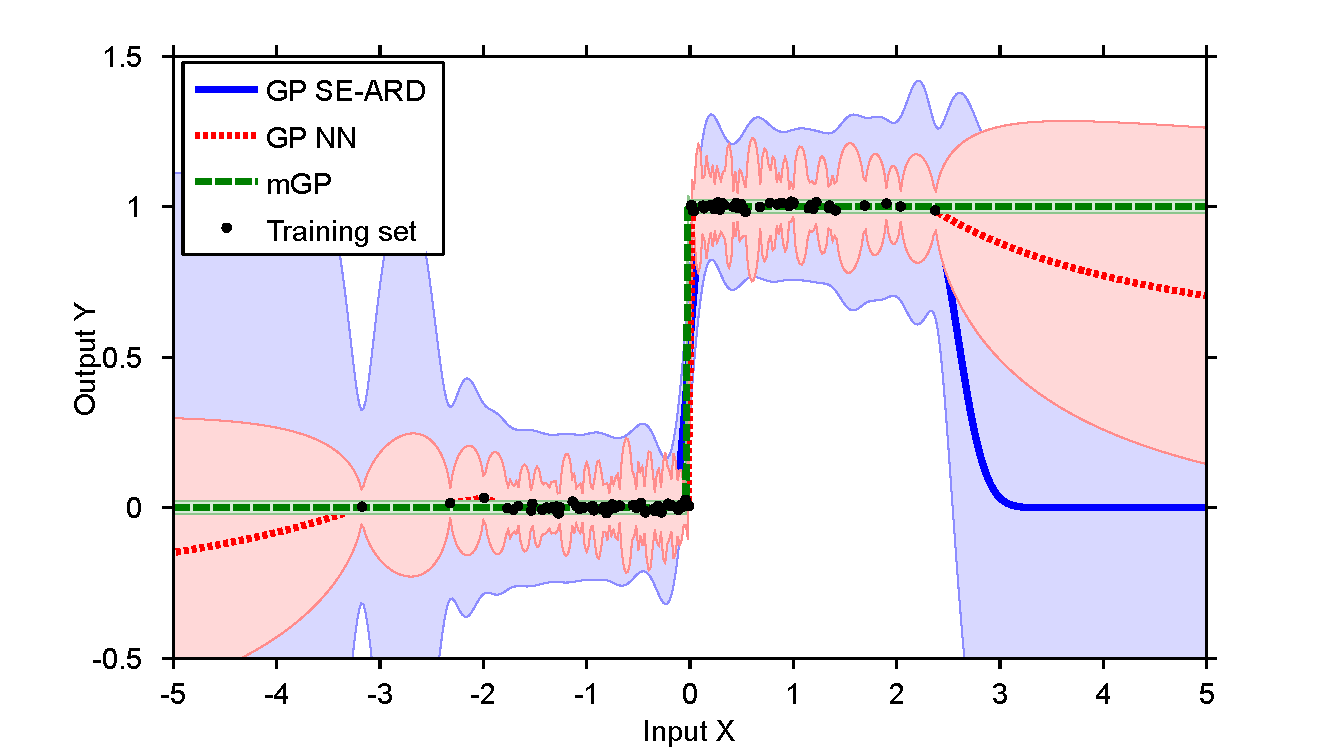
\includegraphics[width=0.7\linewidth]{./images/AAAI2014_0.pdf}
%\label{fig:subfig2}
 \caption{Illustration of a discontinuous function (black dots) that is approximated by three 
 model learning approaches. Classical Gaussian process regression methods (GP SE-ARD, and GP NN) 
 poorly reconstruct this function as they average over the ``jump'', which results in a high model variance. 
 TUD, however, demonstrated that by jointly learning a transformation of the data into a feature space, 
 and a GP regression model from the feature space to observed space, the non-linear function 
 can be reconstructed without large reconstruction errors. 
}
\label{fig:example_discontinuities}
\end{figure}

\subparagraph{Extension and enhancement of the iDyn library. (T1.5)}

The original iDyn library \url{https://github.com/robotology/icub-main/tree/master/src/libraries/iDyn} was designed assuming the robot in a fixed-base configuration. Within CoDyCo the library was redesigned in order to support floating base structures. The associated source code is available here \url{https://github.com/robotology/codyco/tree/master/src/libraries/iDynTree}. Within the YARP and iCub contexts, the libraries are used in the wholeBodyDynamics modules (\url{https://github.com/robotology/icub-main/tree/master/src/modules/wholeBodyDynamics} and \url{https://github.com/robotology/codyco/tree/master/src/modules/wholeBodyDynamicsTree} respectively) to compute simultaneously internal (joint torques) and external (contact) forces and torques. 

\paragraph{Work package 2 progress}

\subparagraph{Definition and design of experimental protocols (T2.1)}

The aim of the work in this task was to provide a solid multidisciplinary base for future research work within CoDyCo. We made a thorough review and summary of the recent relevant literature on human postural control and whole body motion in contact with environment (Delivery 2.1). The review examines postural control strategies without and with additional support contacts, types of perturbations that are commonly used to study neuromuscular functions involved in postural control and reviews the methods for stability evaluation of bipedal systems. The review is concluded with examination of stability metrics that can be applied for non-planar contacts. We plan to extend the review with methods of determination of inertial parameters of human/robot body and submit it for publication in a robotic journal by the end of 2014.

At JSI, we created an experimental setup to study human postural control and whole body motion in contact with environment. We implemented two state-of-the-art methods for perturbation of balance as shown on Figure \ref{fig:exp_protocol_W2} that will allow us to gain understanding how human brain deals with environment in the sense of supportive contacts. Using the same setup we can also validate all biomechanical findings on robotic systems by simply substituting the human subject with a robot. Besides, work has been undertaken to setup experiments also at UB. New equipment (the Moog Hapticmaster robot) was acquired and configured at both JSI and UB. Hapticmaster robot will be used in experiments with compliant and unpredictable contacts.

\begin{figure}
\centering
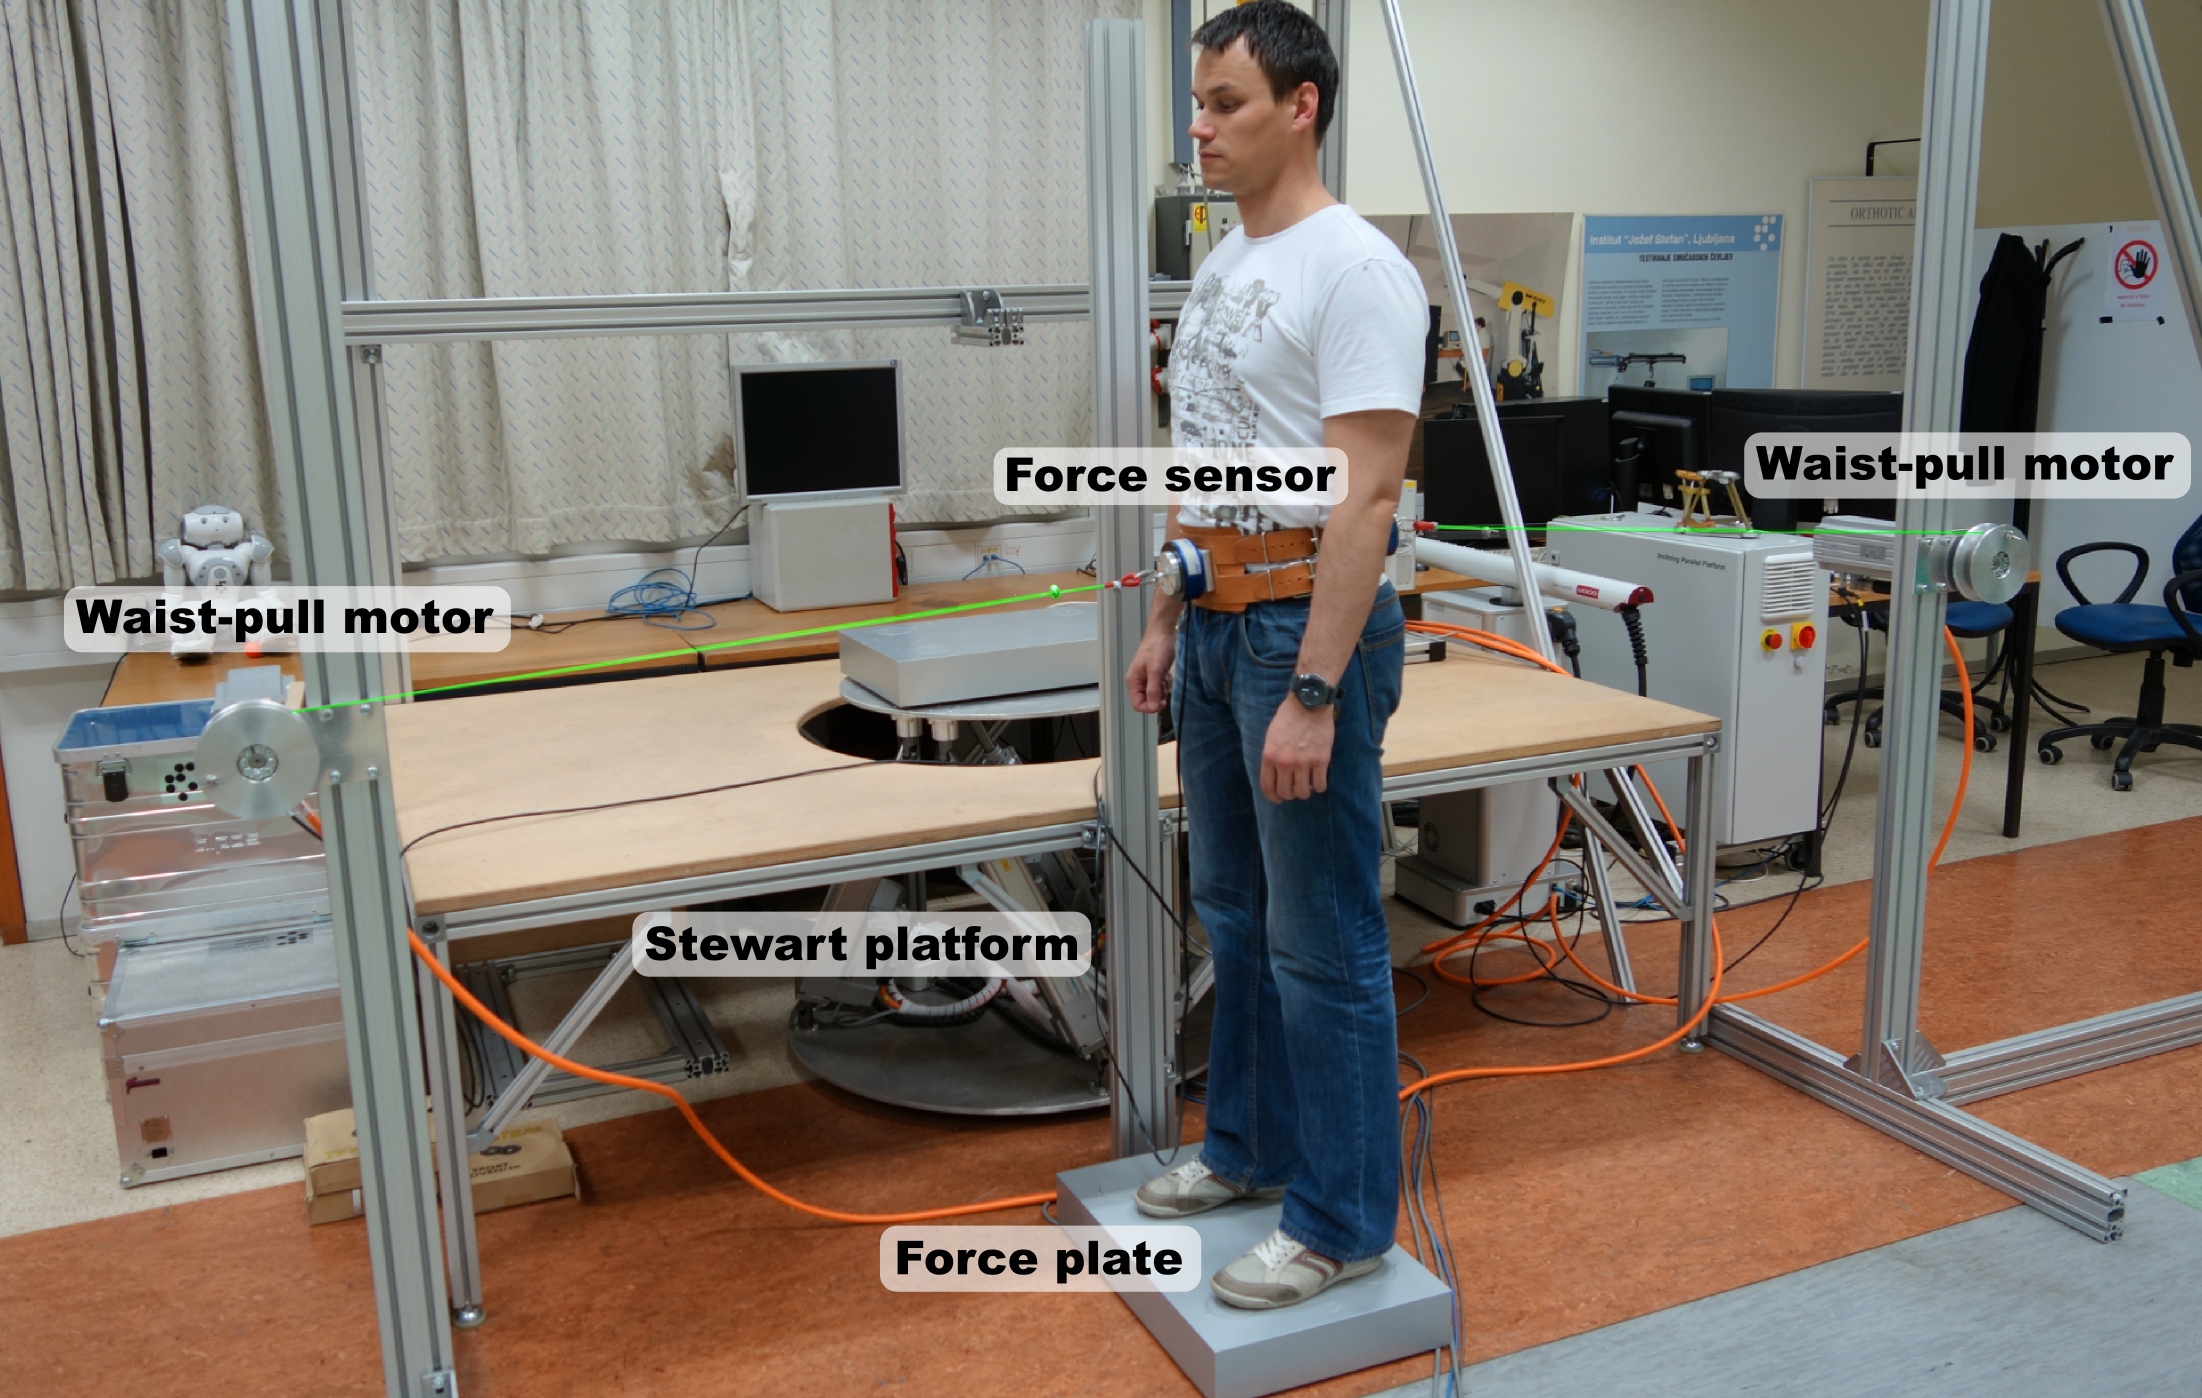
\includegraphics[width=0.8\hsize]{images/exp_setup_WP2.png}
\caption{Experimental setup to study human postural control and whole body motion in contact with environment. Front and back waist-pull motors together with the two force sensors located at the subject's waist allow real-time force perturbations of the subject while the Stewart platform can perturb the balance by either translational or rotational motion (or a combination of both) of the support surface. Force plates are used in combination with kinematical and electromiographical measurements (not on the figure) to study the adaptation of subjects to the given perturbations.}
\label{fig:exp_protocol_W2}
\end{figure}

\subparagraph{Design of models for human whole body motion in contact (T2.2)}

Work has begun on understanding how to derive simplified models of whole-body balance that will encapsulate the task relevant parameters of posture control with multiple contacts. By emulating situations when balance of an individual is challenged, we examined functional role of supportive hand contact at different locations where balance of an individual was perturbed by translational perturbations of the support surface. The experimental methods rested upon our work in Task 2.1 and are depicted on the left side of Figure \ref{fig:exp_paper_W2}.

\begin{figure}
\centering
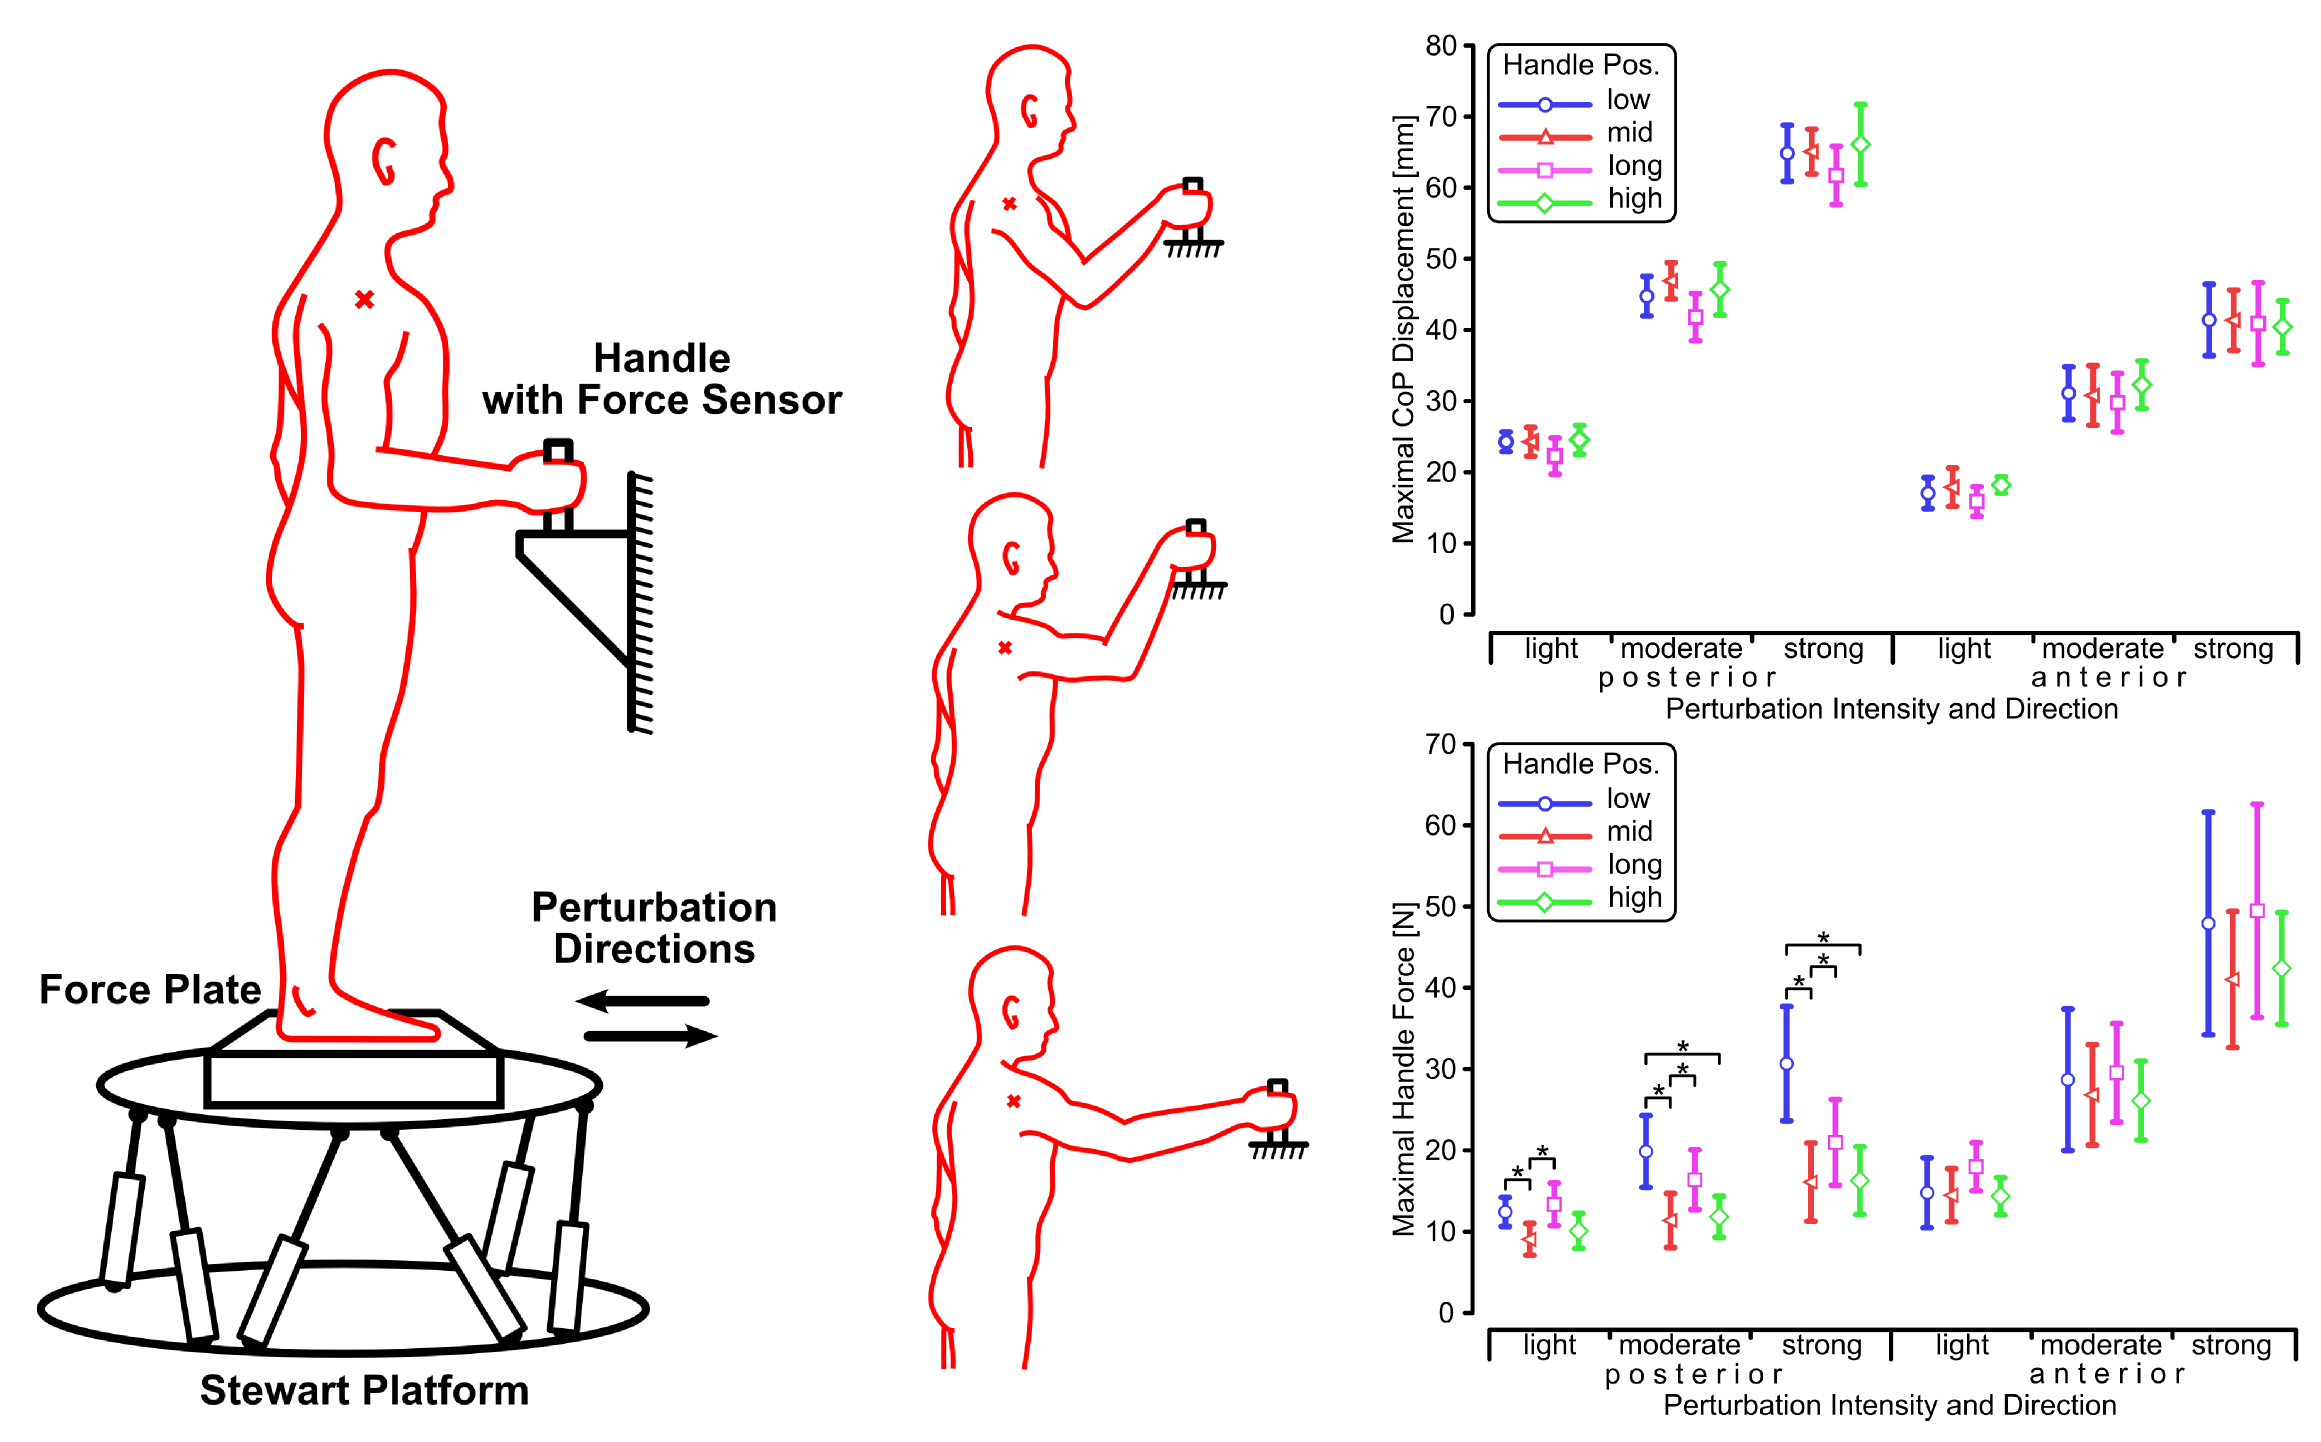
\includegraphics[width=0.8\hsize]{images/exp1_JSI.png}
\caption{Examining functional role of supportive hand contact. The subjects were standing on a force plate mounted on top of the Stewart platform that generated translational perturbations. the subjects were holding the handle with a built-in force sensor in four different positions. Major results of the study are shown on the two diagrams on the right side.}
\label{fig:exp_paper_W2}
\end{figure}

We found that an additional supportive hand contact significantly reduced the maximal displacement of the subject's centre of pressure (CoP) regardless of the position of the handle and the type of the perturbation. On the other hand, the position of the handle had no effects on the maximal CoP displacement (top right diagram on Figure \ref{fig:exp_paper_W2}) which is against the previous belief that the quality of postural control depend on the location of the hand contact \cite{Sarraf2014} and supports the idea that maintaining postural stability is the task of the highest priority and that the central nervous system does whatever necessary to keep the body balanced \cite{Winter1995}. Specifically, subjects always generated the required hand force, no matter where the location of the handle was, to keep the body balanced to the same extent. To get a better understanding of the functional role of supportive hand contacts, we examined the handle forces exerted by the subjects during the perturbation. In contrast with the effects on CoP, we found significant effects of perturbation direction, perturbation intensity and handle position on the maximal force in the handle (bottom right diagram on Figure \ref{fig:exp_paper_W2}). A manuscript with the results of the work in T2.2 was submitted for publication in Gait \& Posture journal in December 2013 and is under review \cite{Babic2014}.

To properly model all these findings we developed a reduced dimensional (6-link, planar) model of a humanoid to be used as an inverse dynamics model for computing joint torques from human experimental data. The detailed analyses based on this model are under way at JSI and UB.

A major challenge of this task is understanding how to determine and measure stability when a human or humanoid robot is in a multi contact situation. The state-of-the-art in postural stability uses traditional metrics such as centre of pressure or zero moment point. However these planar metrics do not apply when there are multiple non-planar contacts. In addition to reviewing the current literature (Task 2.1), we have begun development of new methods for measuring stability margins when a human or humanoid robot has multiple non-planar contacts.

\subparagraph{Human contact choice and learning through physical interaction (T2.4)}

In order to understand how humans make contact choice decisions (e.g. whether or not to initiate a hand contact, and where to place the hand), we need an estimation of joint torques as well as a metric of stability in various multi-contact situations. Thus the work we have begun in Task 2.2 in terms of both simplified models of postural control and metrics of stability, also apply for Task 2.4.

To understand the factors involved in human choice of contact utilization, we performed a series of experiments where the subjects were standing still with arms hanging freely at the sides. The parallel platform induced a randomly timed series of perturbations of different accelerations, velocities and displacements. The aim of the experiments was to investigate what profile of support perturbation forces the human to make a supportive hand contact with environment and how human chooses the location of the hand contact with regard to the direction of the perturbation. Interestingly, we found that the subjects reacted to every perturbation no matter how small or slow the perturbation was or what was the initial acceleration of the perturbation. The reactions were manifested as muscle twitches of shoulder or as unspecific arm motions that were unrelated to the proximity of possible support objects. The reactions occurred also at the smallest perturbations when no actual correction of balance was needed. Our experiments showed that these reactions are essentially protective reactions rather than reactions that have counterbalancing effects \cite{McIlroy1995, Corbeil2013}.

These reactions mask the real factors involved in human choice of contact utilization. We therefore altered the perturbation methods for our further experiments and designed continuous random perturbations in a frequency band that corresponds with typical human motion during postural control \cite{Nawayseh2006}. By doing so we excluded the effect of surprise that evoked the reflex reactions of humans. This will hopefully allow us to uncover the factors involved in human choice of contact utilization.

\paragraph{Work package 3 progress}

The progress for each task are described hereafter.

\subparagraph{Reproducing existing control results in a simple case (T3.1)}
During year one, UPMC has achieved task T3.1 by creating a stand-alone C++ library encapsulating the whole-body controller developed in \cite{salini2012} so that it can be used by all partners in simulation or on (any) real humanoid robot. This version of the controller has been tested in rigid multi-contact scenarios in simulation (see Fig.~\ref{fig:xde}) and is currently adapted for tests on the iCub robot.

\begin{figure*}
\begin{center}
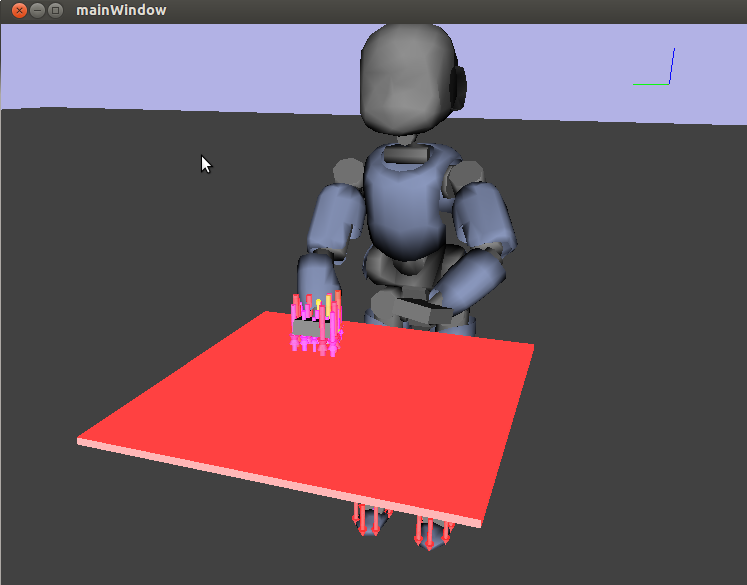
\includegraphics[width=0.3\hsize]{images/s5.png}
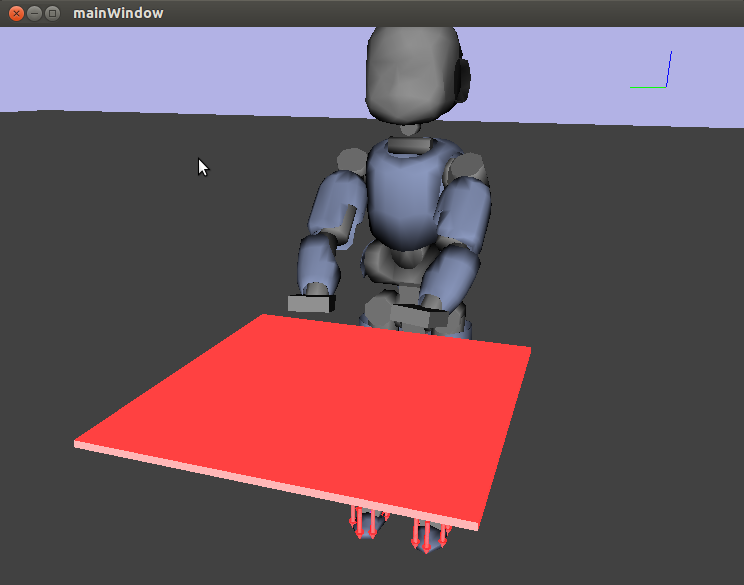
\includegraphics[width=0.3\hsize]{images/s6.png}
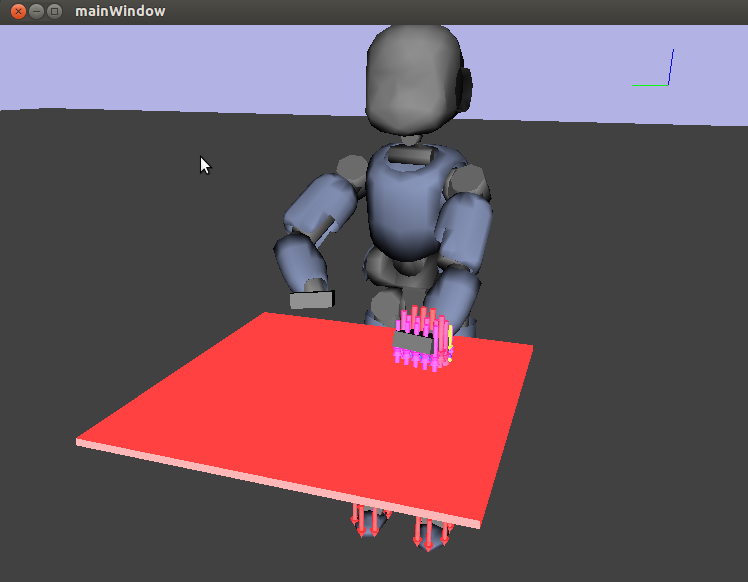
\includegraphics[width=0.3\hsize]{images/s4.png}

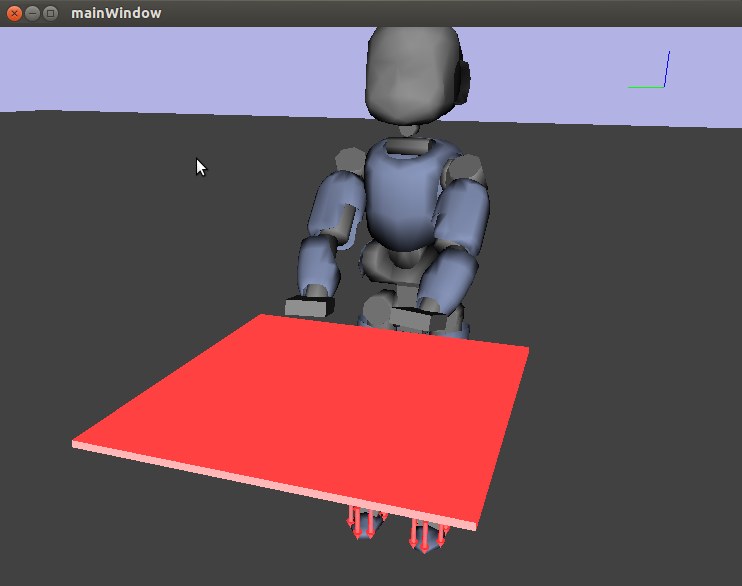
\includegraphics[width=0.3\hsize]{images/s3.png}
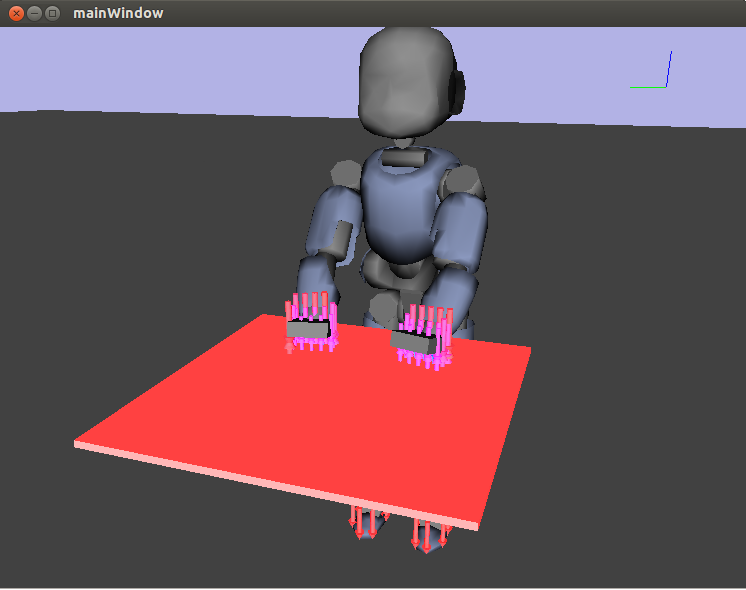
\includegraphics[width=0.3\hsize]{images/s2.png}
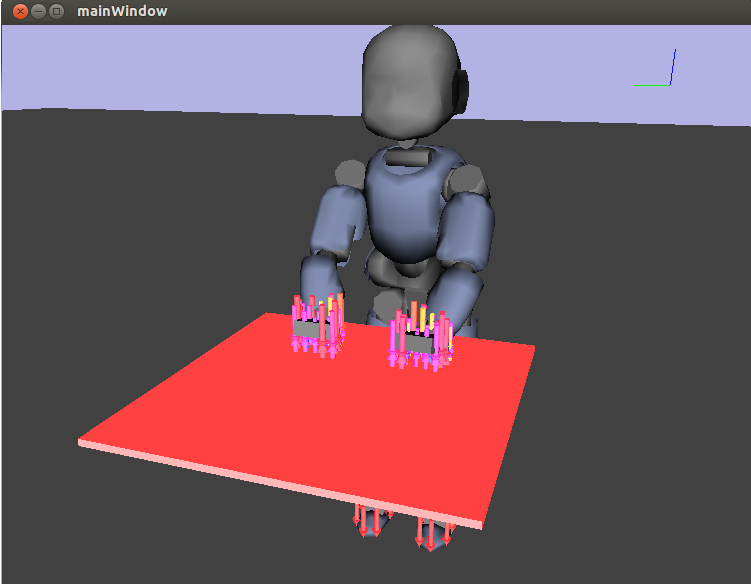
\includegraphics[width=0.3\hsize]{images/s1.png}
\end{center}
\caption{Screenshots of the validation scenario simulated in XDE.}
\label{fig:xde}
\end{figure*}

\subparagraph{Formulating the control problem (T3.2)}

The work performed during year one by UPMC to achieve T3.2 has led to the definition of what a task can be considered to be in the context of the reactive formulation of a multi-task whole body control problem. Among the different characteristics of a task (physical frame, task variable, forward model, desired target trajectory, local controller, priority), the notion of task priority has been largely modified with respect to the classical lexicographic task ordering met in the robotics literature and which is particularly appropriate for cascade resolution approaches such as the one recently proposed in \cite{escande2012}. A partial order has been defined such that task priorities can be described for any pair of task $i$ and $j$. This leads to a richer formulation which includes the original one but is also particularly appropriate for describing task insertion and removal processes as well as priority switching between tasks. Further more, this new prioritization paradigm provides a unique way of defining strict and soft hierarchies between tasks. Associated to this work, the notion  of generalized task projector has been introduced. Each task is associated to a projector which is built based on the tasks priorities. The interest of this projector is that it filters the joint space motion associated to a task so that all priorities are respected, being them soft or strict. Details regarding this work are provided in \cite{liu2013}.

Within this task also IIT contributed with the definition of a software abstraction layer, named wholeBodyInterface (\url{http://wiki.icub.org/codyco/dox/html/namespacewbi.html}). This software library defines the interface to access and control the robot  whole-body. Therefore the wholeBodyLibrary structures the control problem and their definition. Currently the library has been been implemented for both the iCub and the Gazebo iCub simulator.  

\subparagraph{Solving the local control problem (T3.3)}

Associated to the new task formulation proposed in T3.2, the control problem has been formulated by UPMC as an LQP which can be solved by any convex optimization solver dealing with linear constraints. Despite the task hierarchy, the introduction of a generalized task projector per task allows to solve only one LQP. This can be done by introducing as many virtual joint space variables as the number of tasks and using the generalized projector of each task in the expression of the constraints. The resulting problem can be solved by standard convex optimization tools and the cost of introducing virtual joint space variables is compensated for by the fact that only one optimization problem has to be solved. Details regarding this work are provided in \cite{liu2013}.

In the meantime, TUD has proposed to explore optimization methods for solving local control problems that do not require the explicit inversion of any model of the system.  During year one, TUD investigated Bayesian optimization methods that were applied to bipedal locomotion tasks.  One of the key challenges in robotic bipedal locomotion is finding gait parameters that optimize a desired performance criterion, such as speed, robustness or energy efficiency. Typically, gait optimization requires extensive robot experiments and specific expert knowledge. During year one, TUD demonstrated that  data-driven machine learning methods based on Bayesian optimization can be used to automate and speed up the process of gait optimization. These Bayesian optimization methods were used to efficiently find gait parameters that optimize the desired performance metric on a real bipedal walker \cite{calandra2014} and \cite{calandra2014b}.
    

\subparagraph{Bootstrapping and validating the control approach in rigid world and compliant cases (T3.4)}

During year one, UPMC has explored the contribution of MPC approaches to handle the postural balancing problem under varying contact conditions. The hybrid nature of the problem, where varying contact conditions can be accommodated either by adapting the internal forces distribution given a set of contact or by modifying the set of contacts itself, requires control approaches where the desired task trajectories performed through the local, reactive, whole-body controller have to be optimally planned ahead of time in order to provide robust behaviors. The contributions in this domain are mostly related to the work of A. Ibanez \cite{ibanez2013}, \cite{ibanez2014-icra} and \cite{ibanez2014-ark}. The originality of theses contributions lies in:
\begin{itemize}
	\item an augmented ZMP model including external forces exerted directly on indirectly on the center of mass;
	\item a distributed optimization approach that provides a way of generating reference trajectories for the center of mass representing a good compromise given some antagonistic balance and task;
	\item a non scripted foot step placement optimization.
\end{itemize}

UPMC also partially contributed with an experimental study about human behavior during physical contact with the robot. The protocol was registered and obtained the approval of the ethics committee CERES (Conseil d’\'evaluation \'ethique pour les recherches en sant\'e), from University Paris-Decartes. \footnote{Ivaldi et al., "Engagement during human-humanoid interaction", IRB N. 20135200001072.}
The purpose of the experiments is to collect a database of behaviors of experts and naive people interacting physically with the iCub to accomplish a cooperative task. The collected data also include locations of contacts (retrieved through the tactile skin), applied force, robot mouvements: they will be used to study adaptation to human intention during human-robot physical contacts.
    
In the meantime, TUD investigated the interchange of forces during cooperative tasks between humans and robots \cite{berger2013}. Three example scenarios are illustrated in Figure \ref{fig:interaction_tasks}. In such tasks, typically an exchange of forces takes place whenever the interacting agents make contact. Sometimes, forces are even exchanged through an object that is manipulated by both agents, e.g., through a box that is lifted. For a successful execution of such joint physical activities, a robot needs to accommodate for the external forces exerted by a human. To this end, we developed a machine learning approach for identifying external influences and guidance information from humans. During behavior execution by a robot, predictions from a statistical sensor model are continuously compared with stability parameters derived from current sensor readings. Differences between predicted and measured values exceeding the variance of the statistical model are interpreted as perturbations caused by a human and are used to adapt the robot's behavior.
    
\begin{figure}[!ht]
\centering
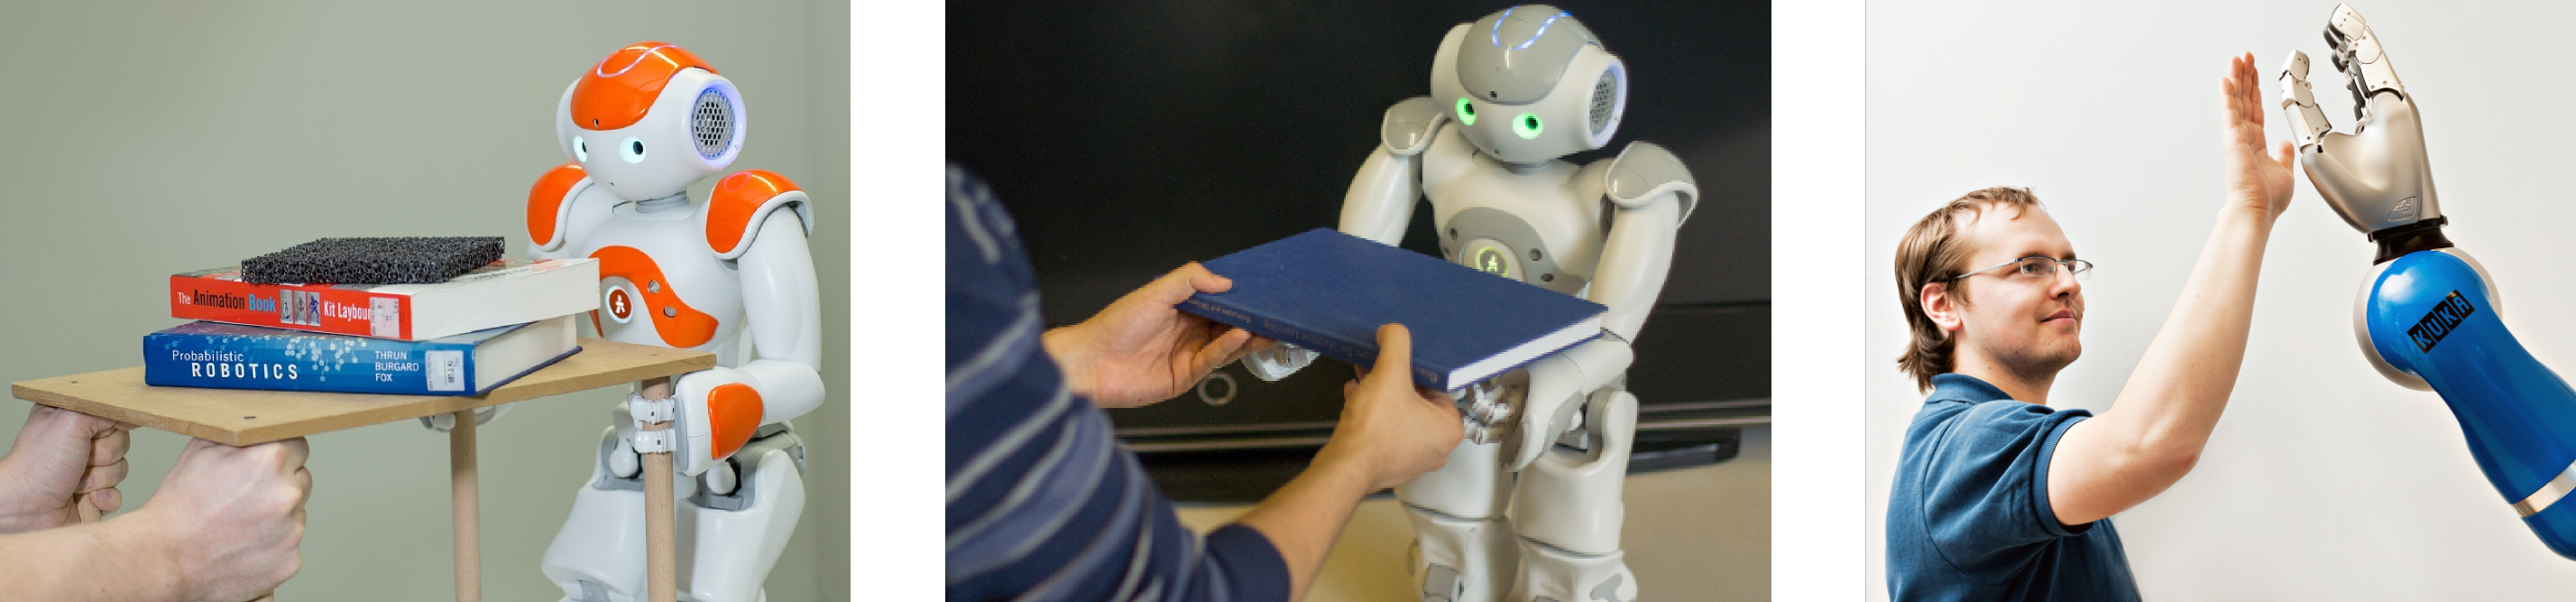
\includegraphics[width=\linewidth]{./images/interaction_wp3.png}
%\label{fig:subfig2}
 \caption{Illustration of three human robot interaction tasks, where an exchange of forces takes place investigated by TUD during year one.
}
\label{fig:interaction_tasks}
\end{figure}

\subparagraph{Deviations from workplan}  

The PM expenses for WP3 after one year of project are globally conform to the planned one. The observed deviations are related to the fact that tasks 3.3 and 3.4 spans the overall duration of the project and the contribution of some of the partners are expected in the 2nd, 3rd and 4th year.

%\emph{\color{red}[For work package 3 (UPMC) provide the following information:]}
%\begin{itemize}
%\item[-] \emph{\color{red}[A summary of progress towards objectives and details for each task;]}
%\item[-] \emph{\color{red}[Highlight clearly significant results;]}
%\item[-] \emph{\color{red}[If applicable, explain the reasons for deviations from Annex I and their impact on other tasks as well as on available resources and planning;]}
%\item[-] \emph{\color{red}[If applicable, explain the reasons for failing to achieve critical objectives and/or not being on schedule and explain the impact on other tasks as well as on available resources and planning (the explanations should be consistent with the declaration by the project coordinator) ;]}
%\item[-] \emph{\color{red}[a statement on the use of resources, in particular highlighting and explaining deviations between actual and planned  person-months per work package and per beneficiary in Annex 1 (Description of Work);]}
%\item[-] \emph{\color{red}[If applicable, propose corrective actions.]}
%\end{itemize}

\paragraph{Work package 4 progress}

\subparagraph{Generalizing and Improving Elementary Tasks with Contacts (T4.3)}

In this task, we aim to generate new skills from data, where elementary skills 
are acquired by imitation learning and transferred to novel situations using 
dynamic systems. During year one, TUD developed a novel representation of 
movement primitives that can be used for imitation learning from noisy observations.
Uncertainty of observed trajectories is explicitely modeled and used to generate new skills.
This movement representation has state-of-the-art capabilities in generalization, 
coupling between the degrees of freedom of the robot, and moreover, 
a time varying feedback controller can be derived in closed form. 
These features are partially illustrated in Figure \ref{fig:promps}.
This work was published
last year at the highly competitive conference on neural information processing \cite{Paraschos_NIPS_2013}.

\begin{figure}[!ht]
\centering
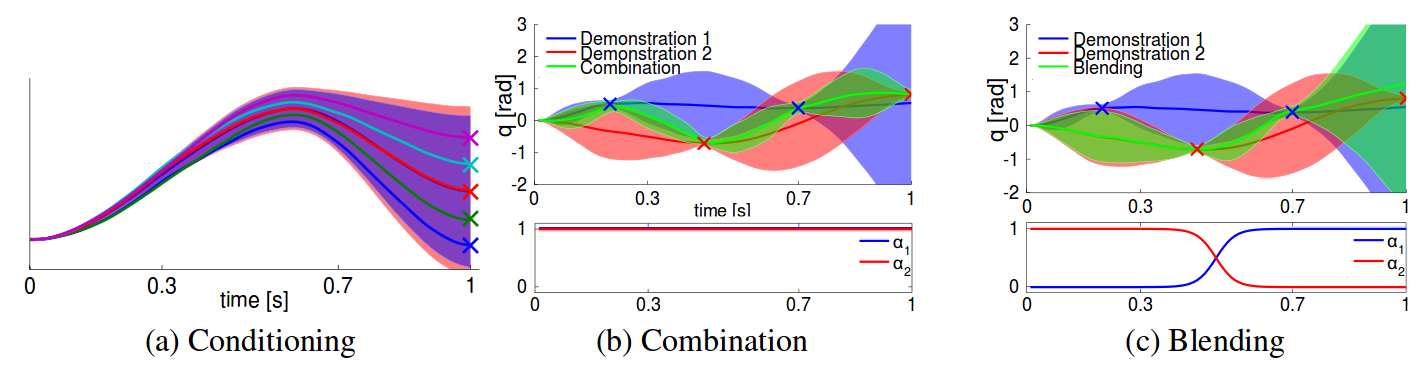
\includegraphics[width=\linewidth]{./images/ProMPs.png}
%\label{fig:subfig2}
 \caption{(a)
Conditioning on different target states. The blue shaded area represents the learned
trajectory distribution. We condition on different target positions, indicated by the ‘x’-markers. The
produced trajectories exactly reach the desired targets while keeping the shape of the demonstrations.
(b)
Combination of two ProMPs. The trajectory distributions are indicated by the blue and red
shaded areas. Both primitives have to reach via-points at different points in time, indicated by
the $x$��-markers. We co-activate both primitives with the same activation factor. The trajectory
distribution generated by the resulting feedback controller now goes through all four via-points.
(c)
Blending of two ProMPs. We smoothly blend from the red primitive to the blue primitive. The
activation factors are shown in the bottom. The resulting movement (green) first follows the red
primitive and, subsequently, switches to following the blue primitive.
}
\label{fig:promps}
\end{figure}

In another work, published at the international conference on humanoid robots (HUMANOIDS), 
TUD demonstrated that this probabilistic approach for trajectory generation
has superior performance against deterministic policies. The use of
probability distributions over the trajectories increased significantly
 the generalization properties, which was evaluated on a high dimensional table
tennis scenario [Paraschos, A. and  Neumann, G and  Peters, J., 2013]. 
In the future work, we plan to incorporate external torque signals to initiate, 
maintain, and terminate contacts.

TUD also investigated how to learn human robot interaction through imitation. We presented a new approach to robot learning that allows anthropomorphic robots to learn a library of interaction skills from demonstration [H Ben Amor, D Vogt, M Ewerton, E Berger, B Jung and J Peters, 2014]. Traditional approaches to modeling interactions assume a pre-specified symbolic representation of the available actions. For example, they model interactions
in terms of commands such as \emph{wait}, \emph{pick-up}, and \emph{place}. Instead of such a top-down approach, we focused on learning responsive behavior in a bottom-up fashion using a trajectory based approach. The key idea behind our approach is that the observation of human-human collaborations can provide rich information specifying how and when to interact
in a particular situation. For example, by observing how two human workmen collaborate on lifting a heavy box, a robot could use machine learning algorithms to extract an
interaction model that specifies the states, movements, and situational responses of the involved parties. In turn, such a model can be used by the robot to assist in a similar lifting task. Our approach is as an extension of imitation learning to multi-agent scenarios, in which the behavior and the mutual interplay between two agents is imitated

\begin{figure}[!ht]
\centering
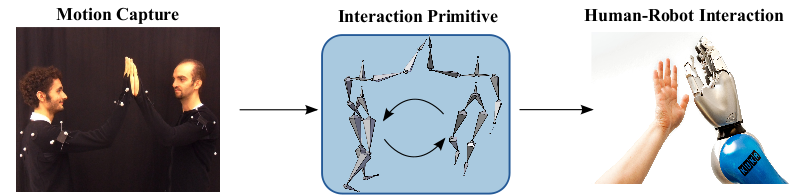
\includegraphics[width=\linewidth]{./images/newoverview.png}
%\label{fig:subfig2}
 \caption{Illustration of the developed interaction primitives that allows to infer the behavior of the interacting partner.
}
\label{fig:interaction_primitives}
\end{figure}

We further extended the above approach by introducing \emph{Interaction Primitives} in [Ben Amor, H.; Neumann, G.; Kamthe, S.; Kroemer, O.; Peters, J., 2014]. Interaction primitives build on the framework of dynamic motor primitives (DMPs) by maintaining a distribution over the parameters of the DMP. With this distribution, we can learn the inherent correlations of cooperative activities which allow us to infer the behavior of the partner and to participate in the cooperation. A conceptual overview is sketched in Figure \ref{fig:interaction_primitives}. A learned Interaction Primitive can be used by a robot to (1) predict the human's next action in the current context, (2) identify the optimal response, (3) synchronize the movement with the human partner.

In the meantime, demonstration-based learning of "optimal trajectories" and stable controllers has been addressed by UPMC, in particular in \cite{stulp2013} where a general, flexible, and compact representation of parameterizable skills is proposed. This work generalizes the standard Dynamic Motor Primitive formulation in \cite{ijspeert2013} and proposes a novel DMP formulation for parametrized skills, based on additionally passing task parameters to the DMP function approximator. This generalizes previous approaches, in particular those which train and execute parametrized skills with two separate regressions. Learning the function approximator with one regression in the full space of phase and tasks parameters allows for more compact models, and the flexible use of different function approximator implementations such as LWPR and GPR, as we demonstrated on the Meka and iCub humanoids robots.

\paragraph{Work package 5 progress}

The activities in WP5 are divided into four tasks corresponding to the four years project duration. As a result, during the first year CoDyCo results concentrate on T5.1. The main result consist in the implementation of the validation scenario consisting of the balancing on different type of rigid contacts.

\subparagraph{Scenario 1: iCub balancing on multiple rigid contacts (T5.1)}

The main contributions to T5.1 have been presented in ``D5.1 Scientific report on validation scenario 1: balancing on multiple rigid contact points.'' which discusses the technical implementation of the first year validation scenario (see \url{https://github.com/robotology-playground/codyco-deliverables/tree/master/D5.1/pdf}). The software developed for the scenario implementation is released with an open-source license and distributed through github (\url{https://github.com/robotology/codyco} ). The main software activities include: a module to identify the whole-body motor transfer functions (\url{https://github.com/robotology/codyco/tree/master/src/modules/motorFrictionIdentification}), a module for estimating whole-body internal (joint torques) and external (contact) forces (\url{https://github.com/robotology/codyco/tree/master/src/modules/motorFrictionIdentification}), a module for whole-body joint torque control (\url{https://github.com/robotology/codyco/tree/master/src/modules/jointTorqueControl}), a C++ library that implements the wholeBodyInterface in simulink (\url{https://github.com/robotology/codyco/tree/master/src/simulink}).

\subparagraph{Deviations from workplan}  

The original work plan have foreseen contacts at feet, hands, back, buttocks, arms and legs. The final validation scenario will only include possible contacts at hands and feet. This simplification is mainly due to the fact that at he end of the CoDyCo first year the iCub does not yet include tactile sensing on the back, legs and buttocks. These sensors will be soon included in the iCub and the CoDyCo software is already designed to include this information. 

%\begin{itemize}
%\item[-] \emph{\color{red}[A summary of progress towards objectives and details for each task;]}
%\item[-] \emph{\color{red}[Highlight clearly significant results;]}
%\item[-] \emph{\color{red}[If applicable, explain the reasons for deviations from Annex I and their impact on other tasks as well as on available resources and planning;]}
%\item[-] \emph{\color{red}[If applicable, explain the reasons for failing to achieve critical objectives and/or not being on schedule and explain the impact on other tasks as well as on available resources and planning (the explanations should be consistent with the declaration by the project coordinator) ;]}
%\item[-] \emph{\color{red}[a statement on the use of resources, in particular highlighting and explaining deviations between actual and planned  person-months per work package and per beneficiary in Annex 1 (Description of Work);]}
%\item[-] \emph{\color{red}[If applicable, propose corrective actions.]}
%\end{itemize}


\paragraph{Work package 6 progress}

Activities within work package 6 achieved the expected results both in terms of administrative activities and management activities. As a major result, the software repository was successfully implemented thanks to novel versioning tool (git) and social coding website (\url{https://github.com}).

\subparagraph{Administrative coordination (T6.1)}
Administration was successfully coordinated by Chiara Andreoli at IIT. The major activity concerned an amendment that the CoDyCo consortium asked the main reason being the fact that Serena Ivaldi, initially hired by UPMC was recently hired by TUD. Part of the administrative coordination activities were also conducted during three main meetings: the kick-off meeting (Genoa, April 5th, 2013), the simulators meeting (Paris, June 5th, 2013) and the midyear meeting (Paris, November 21st-22nd, 2013). Details on the meetings can be found in the CoDyCo website (\url{http://www.codyco.eu}).

\subparagraph{Software repository implementation (T6.2)}

A github software repository was set up \url{https://github.com/robotology/codyco} and the contribution from the different developers can be directly checked in the website. Relevant information can be found also in ``D6.1 Website and repository online'' available here: \url{https://github.com/robotology-playground/codyco-deliverables/tree/master/D6.1/pdf}.


%\begin{itemize}
%\item[-] \emph{\color{red}[A summary of progress towards objectives and details for each task;]}
%\item[-] \emph{\color{red}[Highlight clearly significant results;]}
%\item[-] \emph{\color{red}[If applicable, explain the reasons for deviations from Annex I and their impact on other tasks as well as on available resources and planning;]}
%\item[-] \emph{\color{red}[If applicable, explain the reasons for failing to achieve critical objectives and/or not being on schedule and explain the impact on other tasks as well as on available resources and planning (the explanations should be consistent with the declaration by the project coordinator) ;]}
%\item[-] \emph{\color{red}[a statement on the use of resources, in particular highlighting and explaining deviations between actual and planned  person-months per work package and per beneficiary in Annex 1 (Description of Work);]}
%\item[-] \emph{\color{red}[If applicable, propose corrective actions.]}
%\end{itemize}

\paragraph{Work package 7 progress}

Dissemination and exploitation activities included the participation to international events addressed to both commercial and academic institutions. A preliminary exploitation plan was delineated and reported in the deliverable D7.1.

\subparagraph{Dissemination activities towards academia, industry, and other users (T7.1)}

Dissemination activities were conducted in three main events: (1) iCub exposition at ICRA 2013, IEEE International Conference on Robotics and Automation Karlsruhe, May 6 - 10, 2013; (2) iCub exposition at the European Robotics Forum and Innorobo, Lyon 29th March 2013; (3) iCub exposition at the European Robotics Forum, Rovereto 12th-14th of March 2014. The full list of papers published within CoDyCo can be found here: \url{http://codyco.eu/publications-menu}.

\subparagraph{Exploitation plan (T7.2)}

The first year activities on T7.1 and T7.2 are all contained in ``D7.1 Dissemination and exploitation plan'' available here: \url{https://github.com/robotology-playground/codyco-deliverables/tree/master/D7.1/pdf}.

\subparagraph{Management of IPR (T7.3)}

No activities to be reported during the first year on this task in consideration of the fact that the task started at the very end of the first year. As a minor starting activity the consortium circulated a list containing each partner responsible contact person for the IPR management. This list is contained in ``D7.1 Dissemination and exploitation plan'' available here: \url{https://github.com/robotology-playground/codyco-deliverables/tree/master/D7.1/pdf}.

\subparagraph{Dissemination of a database of human motion with contacts (T7.4)}

During the first year of CoDyCo, IIT completed the task of setting up a database for storing both human and robot datasets. The details on the database are reported in ``D7.2 Standard database with support materials'' available here \url{https://github.com/robotology-playground/codyco-deliverables/tree/master/D7.2/pdf}. 

\section{Second year results}

%!TEX root = ../../secondYearReport.tex


\paragraph*{WP1: toolbox for computing and controlling dynamics of whole-body
  movements with contacts (UB)}

WP1 objectives were achieved for the second year.  In summary, the main
accomplishments and impacts for the research community are as follows:

\begin{itemize}

\item The \texttt{codyco-superbuild} was released as open-source software
  which contains modules for balancing and reaching control for CoDyCo
  project.

\item Several control libraries for the iCub whole-body motion were developed
  and tested both in simulations and on the iCub.

\item An in-situ force/torque sensor calibration procedure was designed to
  improve the accuracy of whole-body identification.  The results are
  published in \cite{Traversaro2015b}.

\item Inertial parameters which are estimated from embedded force/torque
  sensors are used to improve torque estimation of the iCub.  The results are
  outlined in \cite{Traversaro2015}.

\item An experimental software library was released to perform
  maximum-a-posteriori dynamic estimation fusing multiple sensors and encoders
  of the iCub.  Computational efficiency and estimation accuracy of the
  proposed method are studied and published in \cite{Nori2015} and
  \cite{Nori2015b}.
 
 \end{itemize}







%!TEX root = ../../secondYearReport.tex


 
\paragraph*{WP2: understanding and modelling human whole-body behaviours in physical interaction (JSI)}
In T2.2, JSI used the data collected from the biomechanical studies to form a human model for hand-contact assisted balance control in simulation environment. The model serve as platform for devising equivalent robot skills.

In T2.2, UB developed a metric for full-body stability in multiple contact condition. This metric is based on the manipulability of the centre of mass.

In T2.3, JSI developed a novel method for studying human strategies of dealing with contacts with uncertain environment. Instead of performing the contacts with his/her own limbs, the human subject was included into the robot control loop and was asked to perform a task in contact with the environment through the robotic mechanism. To accommodate that, human-robot interfaces were developed. The main advantage of this method, compared to standard biomechanical studies, is that the human observation data can be directly used to build robot skills.

In T2.4, Inria, TUD and UPMC participated in analysing the dataset of the EDHHI experiments where healthy subjects interacted physically with the iCub. The preliminary analysis shows that people, on average, learn quickly how to interact with the robot and move its arms: across three trials, the exchanged forces were smaller and the contacts more precise.

In T2.4, JSI performed a study on multiple healthy subject and analysed the effects of additional supportive contact on full-body balance control. The subjects were continuously perturbed at the waist. In one instance, the subjects did not use any supportive hand contacts while in the other instance, the subject used an additional supportive hand contact. The comparative analysis between the two conditions revealed particular synergies between arm and body muscles which significantly contribute to the improved balance.

In T2.4, TUD and JSI studied whether supporting contacts in human arm reaching tasks are planned or are an effect of a reactive controller. Experiment on multiple subject were performed, where the task was to reach to a target with one hand and use the other hand for additional support. During the experiment, the subject balance was perturbed by a displacement of the ground support.

Finally, in T2.4, UPMC and JSI started an experimental study where the aim is to challenge two well-established but conceptually separated motor control phenomena. We obtained several very promising preliminary results indicating a general mechanism that points out a global trade-off arising from the interactions between movement time, cost and accuracy.

%!TEX root = ../../secondYearReport.tex


 
\paragraph*{WP3: control and optimization of whole-body motion in contact (UPMC)}

After two years of project, the level of achievement of the objectives in WP3 meets the expectations. The main achievements are:
\begin{itemize}
\item[T3.3] \textbf{Studies} by UPMC and UB on the extension of whole-body control frameworks in order to account for non-rigid contacts.  The approach retained by UPMC adapts the desired contact force value and center of mass trajectory in order to establish stable and supporting contacts as fast as possible. This approach assumes a local contact model but does not require the explicit knowledge of its parameters and rather uses the velocity of the contact point to directly adapt the desired contact force. UB computes optimal contact forces based on the momentum of the robot and computes and converts this forces into desired acceleration using an estimated model of the surface in contact. Given these desired accelerations, joint torques are computed in order to best achieve the desired accelerations.
\item[T3.4] \textbf{Integration} by IIT and UPMC of the whole-body controllers on the real robots. This includes a large amount of background work by IIT on low-level control aspects (calibration and identification mostly).
\item[T3.4] \textbf{Investigation} by UPMC of MPC as an efficient mean to optimally handle the postural balancing problem under varying contact conditions.
\item[T3.4] \textbf{Studies} by Inria, TUD and UPMC on the adaptation of task weights in the whole-body controller.
\item[T3.4] \textbf{Studies} by TUD on learning inverse dynamics with contacts to predict contact forces.
\item[T3.4] \textbf{Studies} by UB on projected operational space dynamics for the control of constrained motion for a manipulator performing a task while in contact with the environment.
\end{itemize}




%!TEX root = ../../secondYearReport.tex


\paragraph*{WP4: adaptation, generalization and improvement of compliant control and tasks with contacts (TUD)}

The goal of WP4 is to endow the CoDyCo humanoid robot control architecture with
the core abilities for the adaptation, generalization and self-improvement of
both control laws and tasks that involve physical interaction with humans, and
the environment.

%withot inv dyn learning (inv dyn learning is part of WP3)
During the second year, IIT developed a theoretical framework for estimating whole-body
dynamics from distributed multimodal sensors \cite{Nori2015}.
TUD continued their research in probabilistic movement
primitive representations. A journal article on imitation learning and the
co-activation of basic skills is under review. For multi-modal solutions an
extension using mixtures of Gaussians with latent variables was published at an
international robotics conference \cite{Rueckert_2015}. In tasks with
contacts, a model-free probabilistic movement representation was developed that
models joint distributions over kinematic and force trajectories. This work is
under review. Further, TUD investigated noise robust planning methods methods to
plan movement skills given task-space constraints. This work was published at an
international humanoid robot conference \cite{Rueckert2014} and will be
used in year three for generating optimal control laws with learned dynamics
models. During year two, TUD investigated the learning of temporal activation
profiles of low-level task controller. This work is under review. 
A similar line of research was conducted by UPMC who studied how to deal with interferences in task combinations in whole-body.
The tasks are parameterized with Dynamical Movement Primitives, whose parameters are optimized
based on a general compatibility principle. This work was published at an 
international humanoid robot conference \cite{lober-HUMANOIDS2014}. 
In a second study that is currently under review, UPMC studied how task
variability can be used to modulate task priorities during their execution. 
UB continued their research on computed torque control leveraging low-gain control. 
%!TEX root = ../../secondYearReport.tex

\paragraph*{WP5: systems integration, standardization and evaluation on the iCub robot (IIT)}

The second year WP5 activities have concentrated on the second year validation scenario. A complete description of the scenario can be found in ``D5.2 Scientific report on validation scenario 2: balancing on feet while performing goal directed actions.'' which discusses the technical implementation of the second year validation scenario (see \url{https://github.com/robotology-playground/codyco-deliverables/tree/master/D5.2/pdf}). With respect to the state of the art the work progress represents a step towards whole-body torque control under postural, contacts and goal-directed constraints. The integration of tactile feedback within the whole-body controller is a peculiarity of the implemented CoDyCo validation scenario and therefore represents yet another step forward with respect to the current state of the art. 
%!TEX root = ../../secondYearReport.tex


\paragraph*{WP6: management (IIT)}

The CoDyCo project continued successfully. Management activities included the definition of a second amendment procedure smoothly organized by the consortium and the project officer. The software repository (\url{https://github.com/robotology/codyco}) have been significantly improved as clearly documented in the web-based git repository hosting service (\url{https://github.com}). 
%!TEX root = ../../secondYearReport.tex


\paragraph*{WP7: dissemination and exploitation (IIT)}

Within WP7, CoDyCo second year achievement include: dissemination at relevant academic and industrial events; population of the CoDyCo database to disseminate robot and humans datasets. 

%!TEX root = ../../isa_padois_et_al.tex


\paragraph{Work package 1 progress}

\subparagraph{Software architecture design and evaluation of available
  open-source software pertinent to the scope of the project. (T1.1)} 

The goal of T1.1 was to agree on a specific software architecture with
associated software tools whose specifications, dependencies and
interconnections meet the requirements and needs for achieving the goals of
the project.  The software, which is called \texttt{codyco-superbuild}, is
available via github on \url{https://github.com/robotology/codyco-superbuild}.
The modules and specifications of the software are as follows:

\begin{itemize}
\item \texttt{codyco-commons}: A collection of functions and utilities used in
  the other projects
\item \texttt{idyntree}: YARP-based Floating Base Robot Dynamics Library
\item \texttt{paramHelp}: Library for simplifying the management of the
  parameters of YARP modules
\item \texttt{wholebodyinterface}: C++ Interfaces to sensor measurements,
  state estimations, kinematic/dynamic model and actuators for a floating base
  robot
\item \texttt{yarp-wholebodyinterface}: Implementation of the
  wholeBodyInterface for YARP robots
\item \texttt{WBI-Toolbox}: Simulink Toolbox for rapid prototyping of Whole
  Body Robot Controllers
\item \texttt{codyco-modules}: YARP modules and controllers developed within
  the CoDyCo project
\end{itemize}


\subparagraph{Simulator for whole-body motion with contacts (T1.2)}

The CoDyCo project requires a modular, component-based dynamics simulation
software providing numerically stable, computationally efficient and
physically consistent simulations of whole-body virtual human(oid) systems in
contact with rigid or soft environments.  To this end, in year one, a new iCub
simulator was released and documented as part of deliverable D1.1.


\subparagraph{Control library for flexible specification of task space
  dynamics of floating base manipulators. (T1.3)}

During the second year both IIT and UPMC contributed to the development of
several software components for controlling the iCub whole-body behavior.
UPMC has continued the integration of its whole-body controller within the
overall software architecture by properly connecting to the WholeBodyInterface
developped by IIT and described in Deliverable~1.2.  Tests of this integration
has been performed both in the Gazebo simulator as well as on the iCub robots
present at UPMC.


\subparagraph{System dynamics estimation software. Extension to
environmental compliance estimation (T1.4)}

The goal of this task is to develop a software tool for on-line identification
of whole-body dynamics, as well as the compliance of contacts established
between the robot and the environment.

\begin{itemize}
\item Within T1.4, IIT continued the activities started during the previous
  year, with specific focus on whole-body identification \cite{Traversaro2013,
    Traversaro2014}.  In order to enhance the identification accuracy, an
  in-situ force/torque sensor calibration procedure was designed
  \cite{Traversaro2015b} (see Fig.~\ref{fig:validation}) and implemented in a
  software
  component\footnote{\url{https://github.com/robotology-playground/insitu-ft-calibration}.}
  which has been released with an open source license.  Similarly, in order to
  enhance the torque estimation accuracy, IIT conducted a theoretical analysis
  that exploits embedded force/torque sensors.  It has been proven
  \cite{Traversaro2015} that the inertial parameters estimated from embedded
  force/torque sensors can be successfully used for torque estimation.
\item During year two, TUD worked with the WBI toolbox in Matlab to study
  whole-body controllers capable of integrating learned inverse dynamics
  models.  The idea, more specifically, is to combine the low-level torque
  control at joint level with the learned dynamics models of WP4 (T4.2), which
  can thus provide the correct torques for rigid and compliant contacts.  TUD
  implemented a whole-body impedance controller and two balance controllers
  with the WBI toolbox in Matlab (see Figure~\ref{fig:wbitud}).  The
  controllers were tested on Gazebo and on the iCub mex model simulated in
  Matlab.  The integration with the outcome of WP4 is ongoing.
\end{itemize}

\begin{figure}[h]
\vspace{0.5em}
\centering
{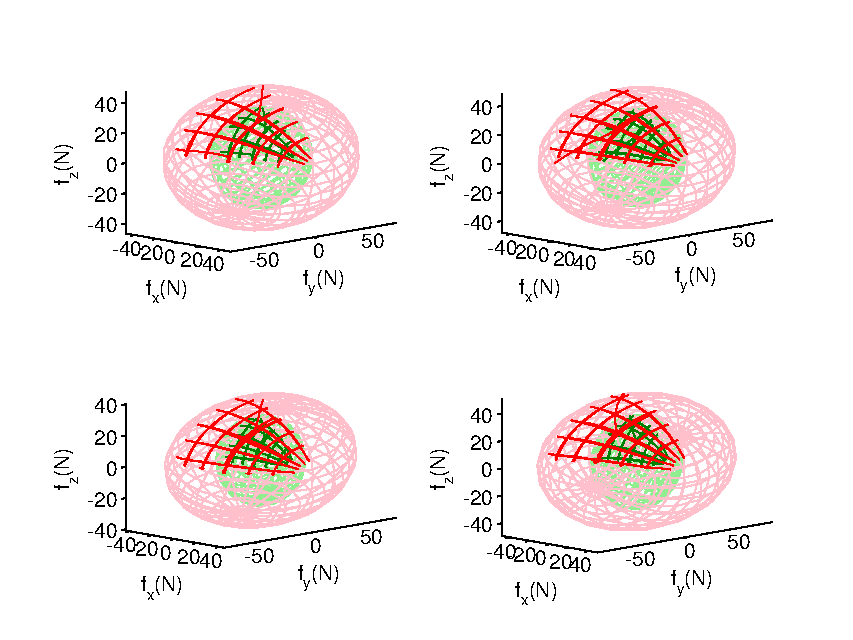
\includegraphics[width=\linewidth]{images/leg_validation.pdf}}
\caption{The image shows the accuracy in calibrating the force/torque sensor
  with the procedure described in \cite{Traversaro2015b}. The four plots refer
  to four different experimental conditions (different values for the
  calibration weights).  Ideally, perfectly calibrated data should lie on the
  surface of a three dimensional sphere. Dark green: force measurements
  obtained with the calibration matrix estimated using the proposed
  technique. Dark red: force measurements obtained with the calibration matrix
  provided with the sensor.  Light red and light green surfaces: ellipsoids
  fitted to the measured forces.  Qualitative calibration accuracy can be
  obtained by looking at the spherical symmetry of the fitted ellipsoids.}
\label{fig:validation}
\end{figure}

 \begin{figure}
 \centering
 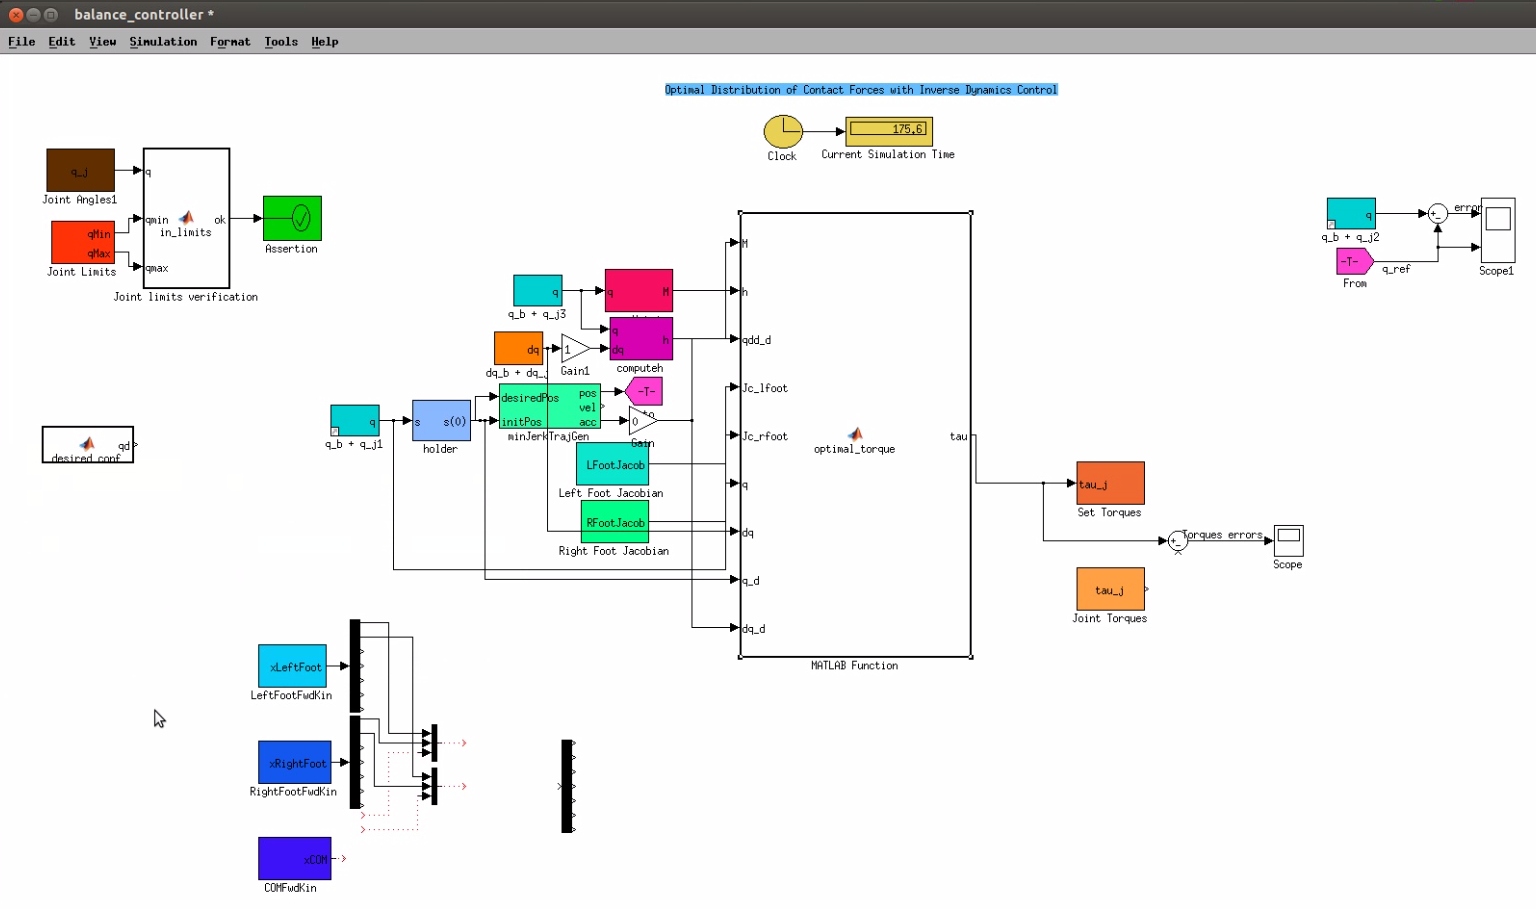
\includegraphics[width=\linewidth]{images/wbi_torque_controller.png}
  \caption{One of the balance controllers implemented by TUD with the WBI
    toolbox in Matlab.  }
 \label{fig:wbitud}
 \end{figure}


\subparagraph{Extension and enhancement of the iDyn library. (T1.5)}
\label{sec:T15}
 
The goal of this task is to provide a reliable software tool for on-line
estimation of whole-body dynamics.  Before CoDyCo, dynamic estimations on the
iCub were relying on the iDyn software
library\footnote{\url{https://github.com/robotology/icub-main/tree/master/src/libraries/iDyn}.},
designed for fixed-base robots.  Within the first year of CoDyCo,
iDynTree\footnote{{\url{https://github.com/robotology/codyco/tree/master/src/libraries/iDynTree}}.}
was released in response to the need of representing floating base structures.
During the second year of the project, we investigated on the problem of
extending iDynTree to the case of multiple redundant sensors.  The
investigation resulted in an experimental software
library\footnote{\url{https://github.com/iron76/bnt_time_varying}.} currently
implemented in \textsc{Matlab}.  The software performs maximum-a-posteriori
dynamic estimation fusing multiple sensors such as gyroscopes, linear
accelerometers, embedded force-torque sensors and encoders.  Computational
efficiency is obtained by exploiting the sparsity of the underlying problem
\cite{Nori2015} (see Fig.~\ref{fig:varTimeComplete}).  Estimation accuracy is
obtained by a modified version of the expectation maximisation algorithm
\cite{Nori2015b} (see Fig.~\ref{fig:extForceEstimation}).

\begin{figure}
   \centering
   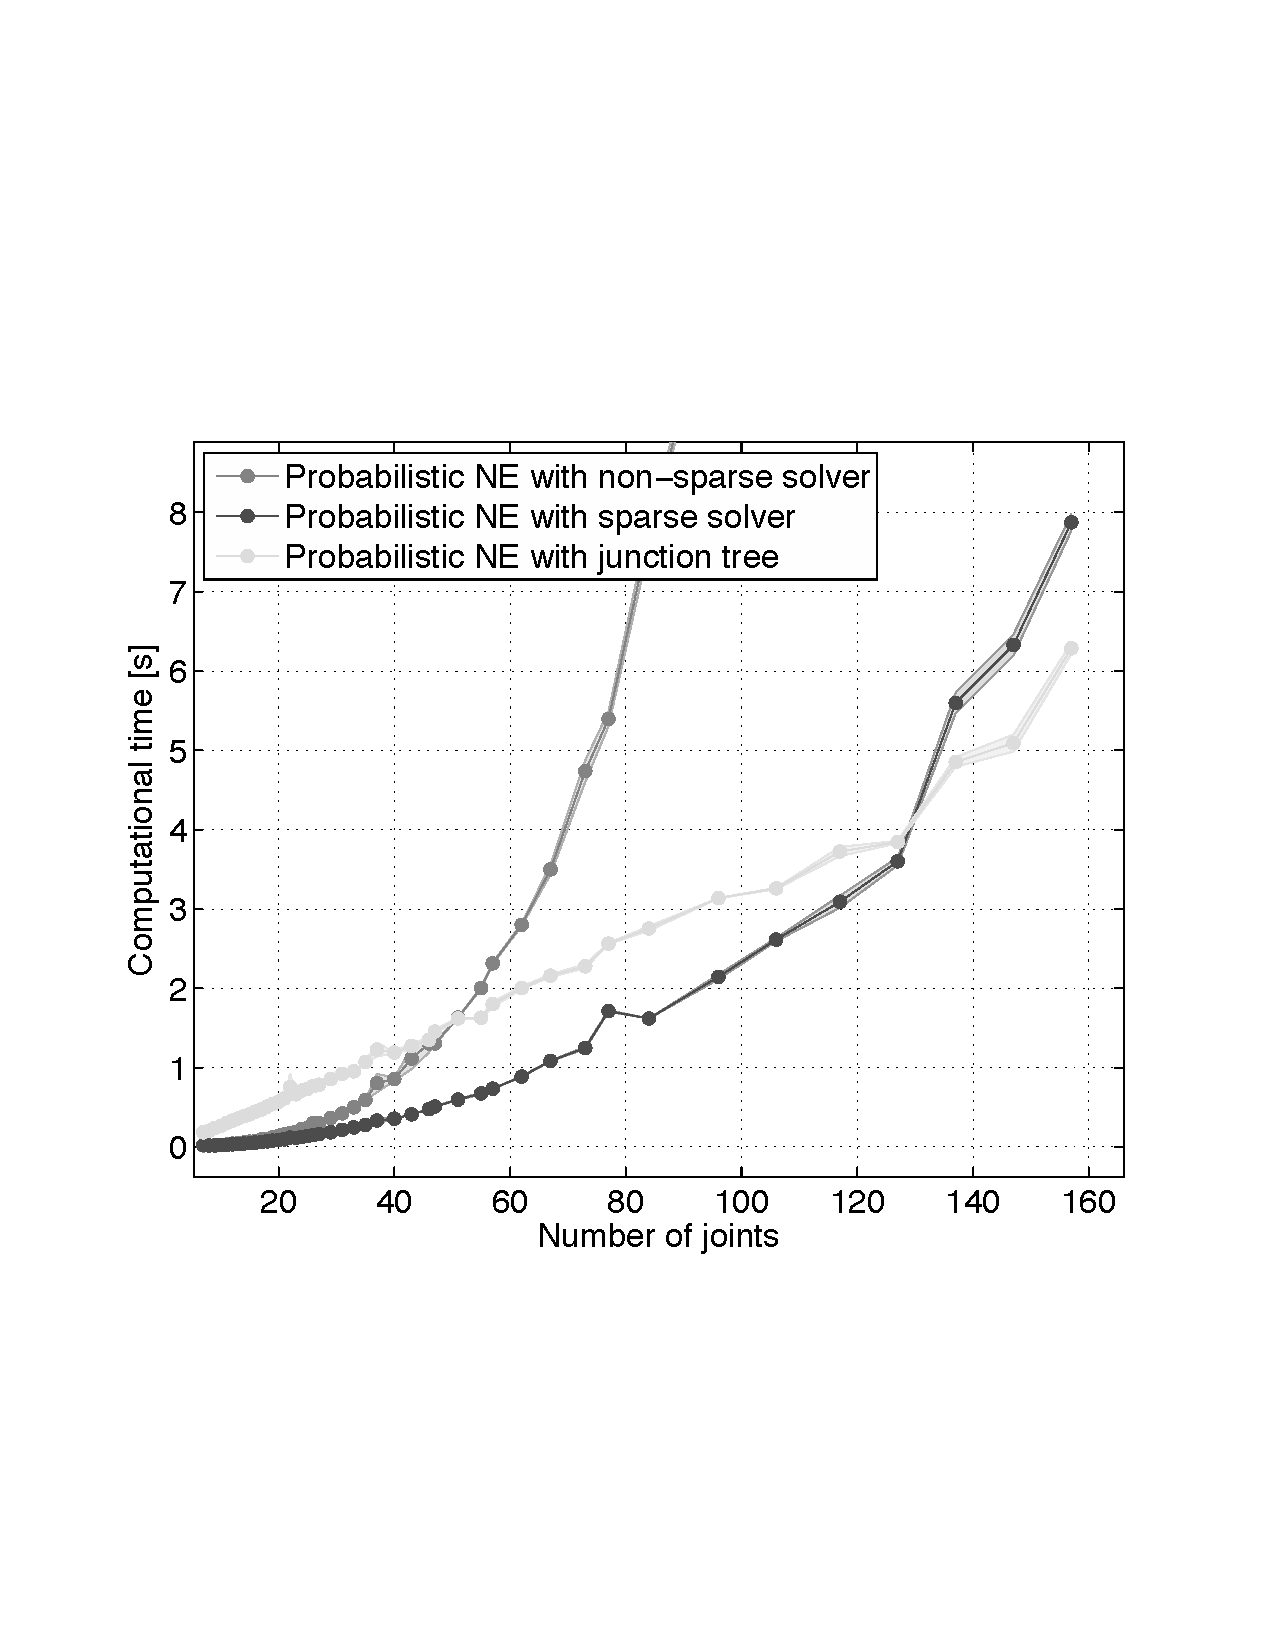
\includegraphics[width=\linewidth]{images/varTimeComplete.pdf}
   \caption{\label{fig:varTimeComplete} Comparison of non-sparse (S1-gray),
   sparse (S2-dark-gray) and Bayesian network junction tree (S3-light-gray)
   solvers in solving maximum-a-posteriori dynamics with redundant
   measurements (see \cite{Nori2015} for details).}
\end{figure}

\begin{figure*} [!ht]
  \centering
  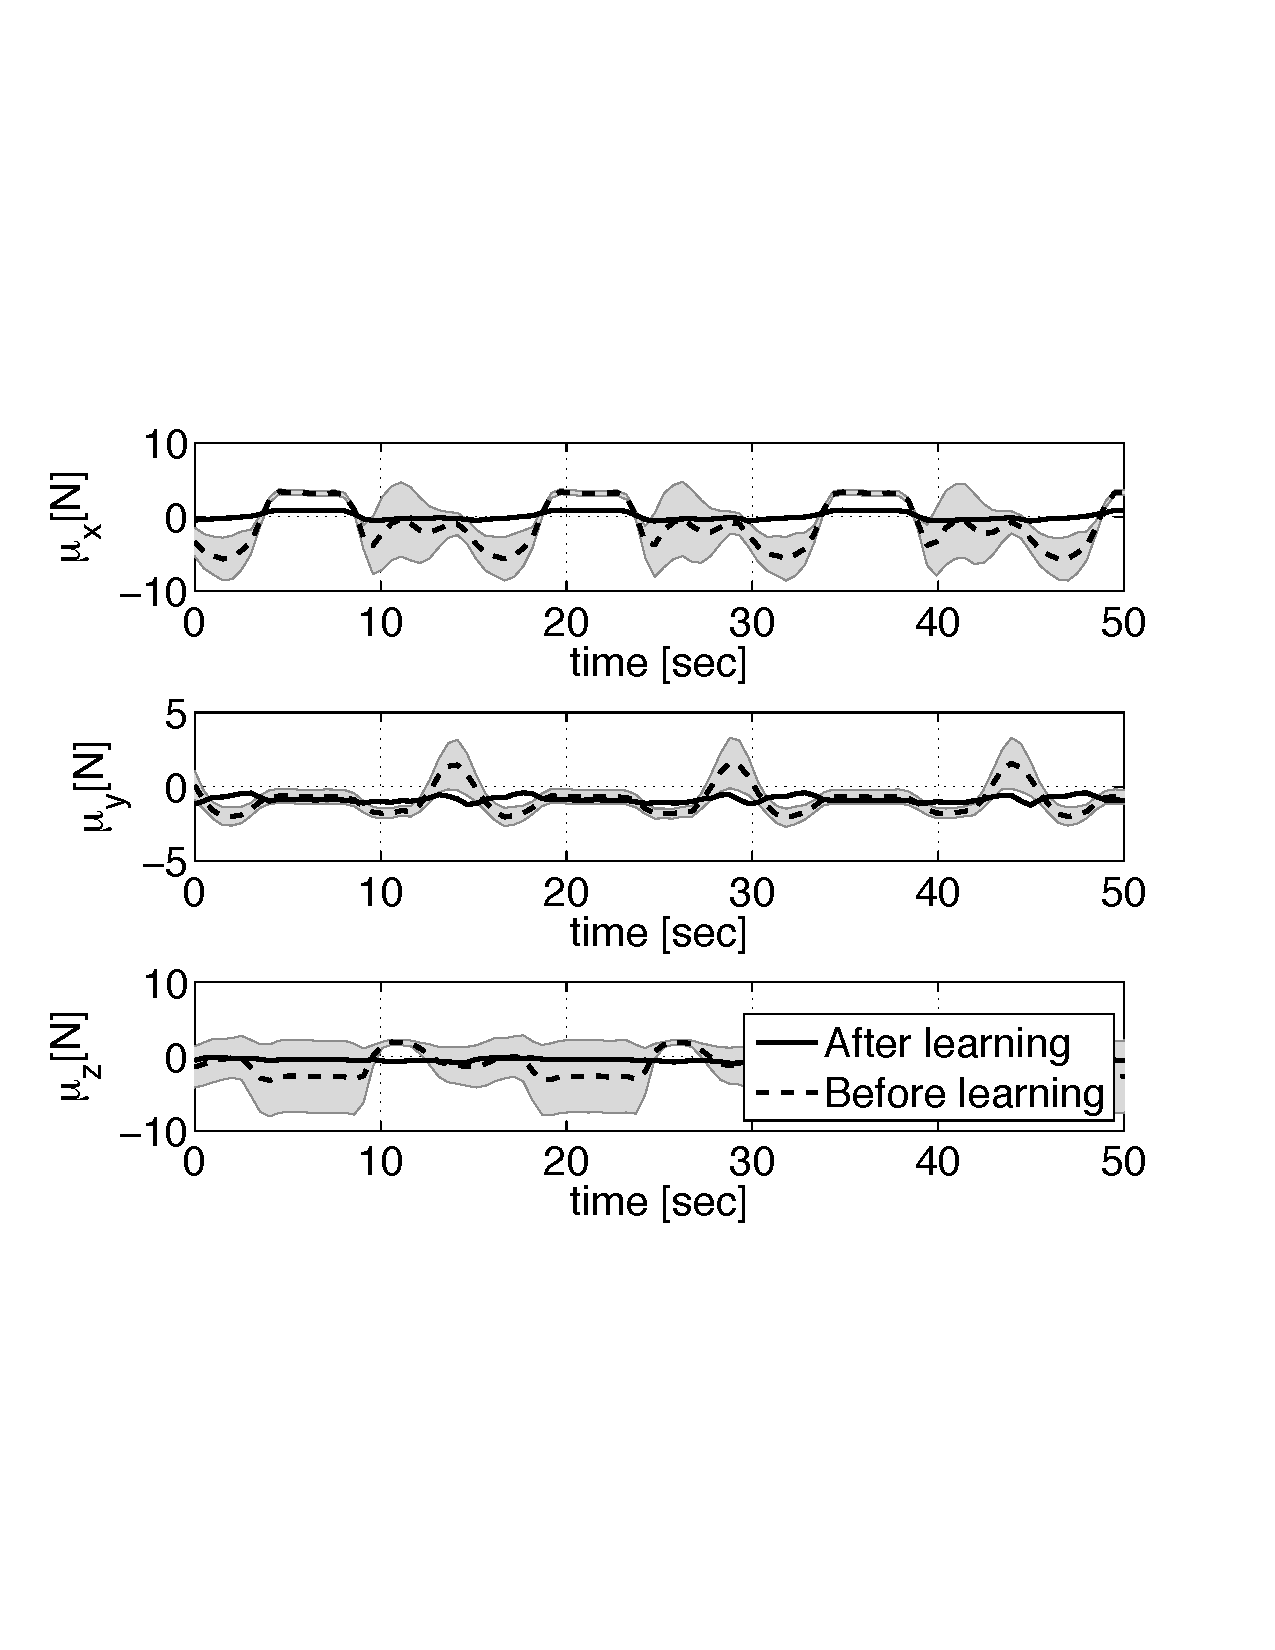
\includegraphics[width=0.45\linewidth]{images/torques.pdf}
  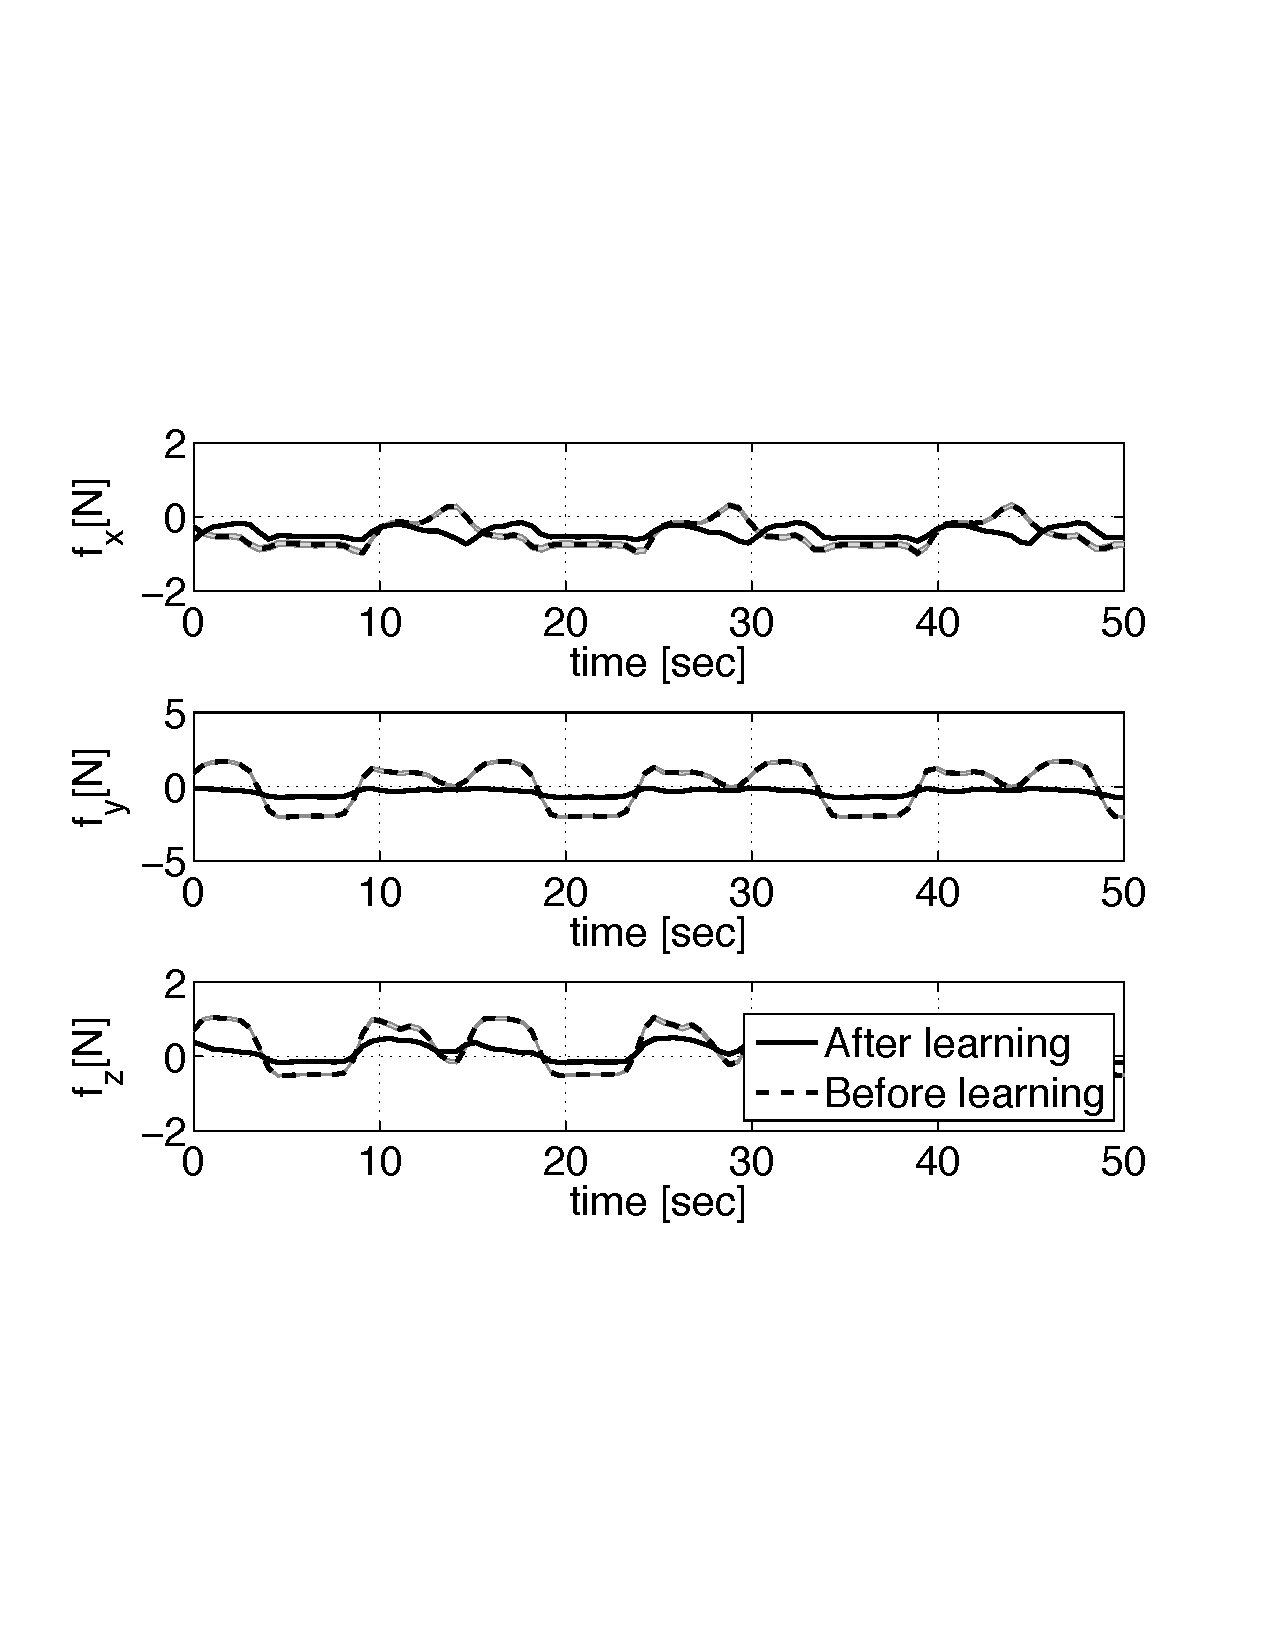
\includegraphics[width=0.45\linewidth]{images/forces.pdf}
  \caption{\label{fig:extForceEstimation} The picture shows the errors in
  estimating an external wrench.  The two curves refer to the estimation
  obtained before (dashed line) and after (solid line) the estimation of the
  data covariance with a modified EM algorithm \cite{Nori2015b}.}
\end{figure*}












%%!TEX root = ../../secondYearReport.tex


\subparagraph{Resources}
Overall, the use of resources within WP1 was in accordance to the plans. 

\begin{center}
  \begin{tabular}{|C{1.5cm}|C{1.5cm}|C{1.5cm}|C{2cm}|C{2cm}|C{2cm}|C{2cm}|}
    \hline \footnotesize \textbf{WP1 person months}& \footnotesize
    \textbf{IIT}&\footnotesize \textbf{TUD}&\footnotesize \textbf{UPMC}&
    \footnotesize \textbf{UB} &\footnotesize \textbf{JSI} & \footnotesize \textbf{INRIA}\\
    \hline \footnotesize Year 1 & 8.67 &1.00 & 3.29 & 0.51 & 2.00 & -\\
    \hline \footnotesize Year 2 & 3.00 & 3.00 & 0.48 & 2.29 & 0.00 & 0.00 \\
    \hline \footnotesize Partial & 11.67 & 4.00 & 3.77 & 2.8 & 2.00 & 0.00\\ \hline
    \hline \footnotesize Overall & 12.00 & 9.00 & 6.00 & 15.00 & 6.00 & 5.00 \\
    \hline
  \end{tabular}
\end{center}

\subparagraph{Deviations from workplan} 
No significant deviations. 


%!TEX root = ../../secondYearReport.tex
\paragraph{Work package 2 progress}


\subparagraph{Design of models for human whole body motion in contact (T2.2)}
In the scope of T2.2, JSI created a 3D dynamic model of a human holding to a stable object during continuous perturbations of stance. The model was devised from measurements on 13 male subjects. Using the kinematical data recorded with frequency of 100Hz, forces that the subjects excerted on the ground, and the forces in the handle, we performed an inverse dynamic procedure and obtained joint torques produced by muscles during the experiment. An illustration of the model is shown in Fig. \ref{fig:skeleton}. Using this modelling approach we are now able to efficiently study the biomechanics of humans in contact with the environment.

\begin{figure}[!t]
	\begin{center}
		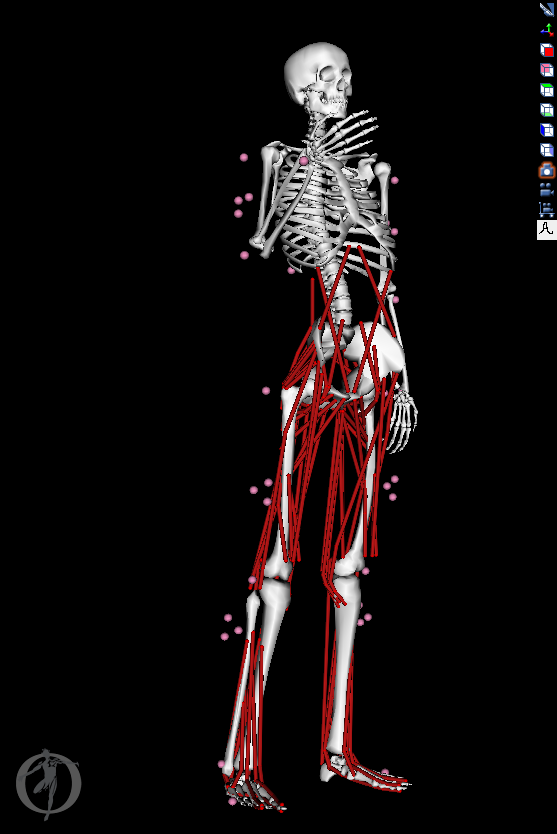
\includegraphics[width=0.5\textwidth]{images/skeleton_v1.png}
		\caption{Model of a subject holding a handle.}
		\label{fig:skeleton}
	\end{center}
\end{figure}


During the second year of the project, UB studied the effects of hand contact
on the stability of a planar humanoid robot (see Fig.~\ref{planarhumanoid})
while a momentum based controller is used to control the robot's balancing
motion \cite{Azad2014}. They compared the simulation results with the
results of the experiments on human subjects which are reported in
\cite{Babic2014}. Both simulations and experiments agreed that different
values of hand contact forces in different hand positions cause the same
displacements of the CoP of the foot. This implies that regulating the CoP of
the foot has the highest priority for both humans and the momentum based
controller.  This study suggested that the momentum based controller is an
adequate controller to replicate human behaviour during balancing motions.

\begin{figure}[!t]
  \centering
	\begin{subfigure}[b]{0.45\textwidth}
	\centering
  	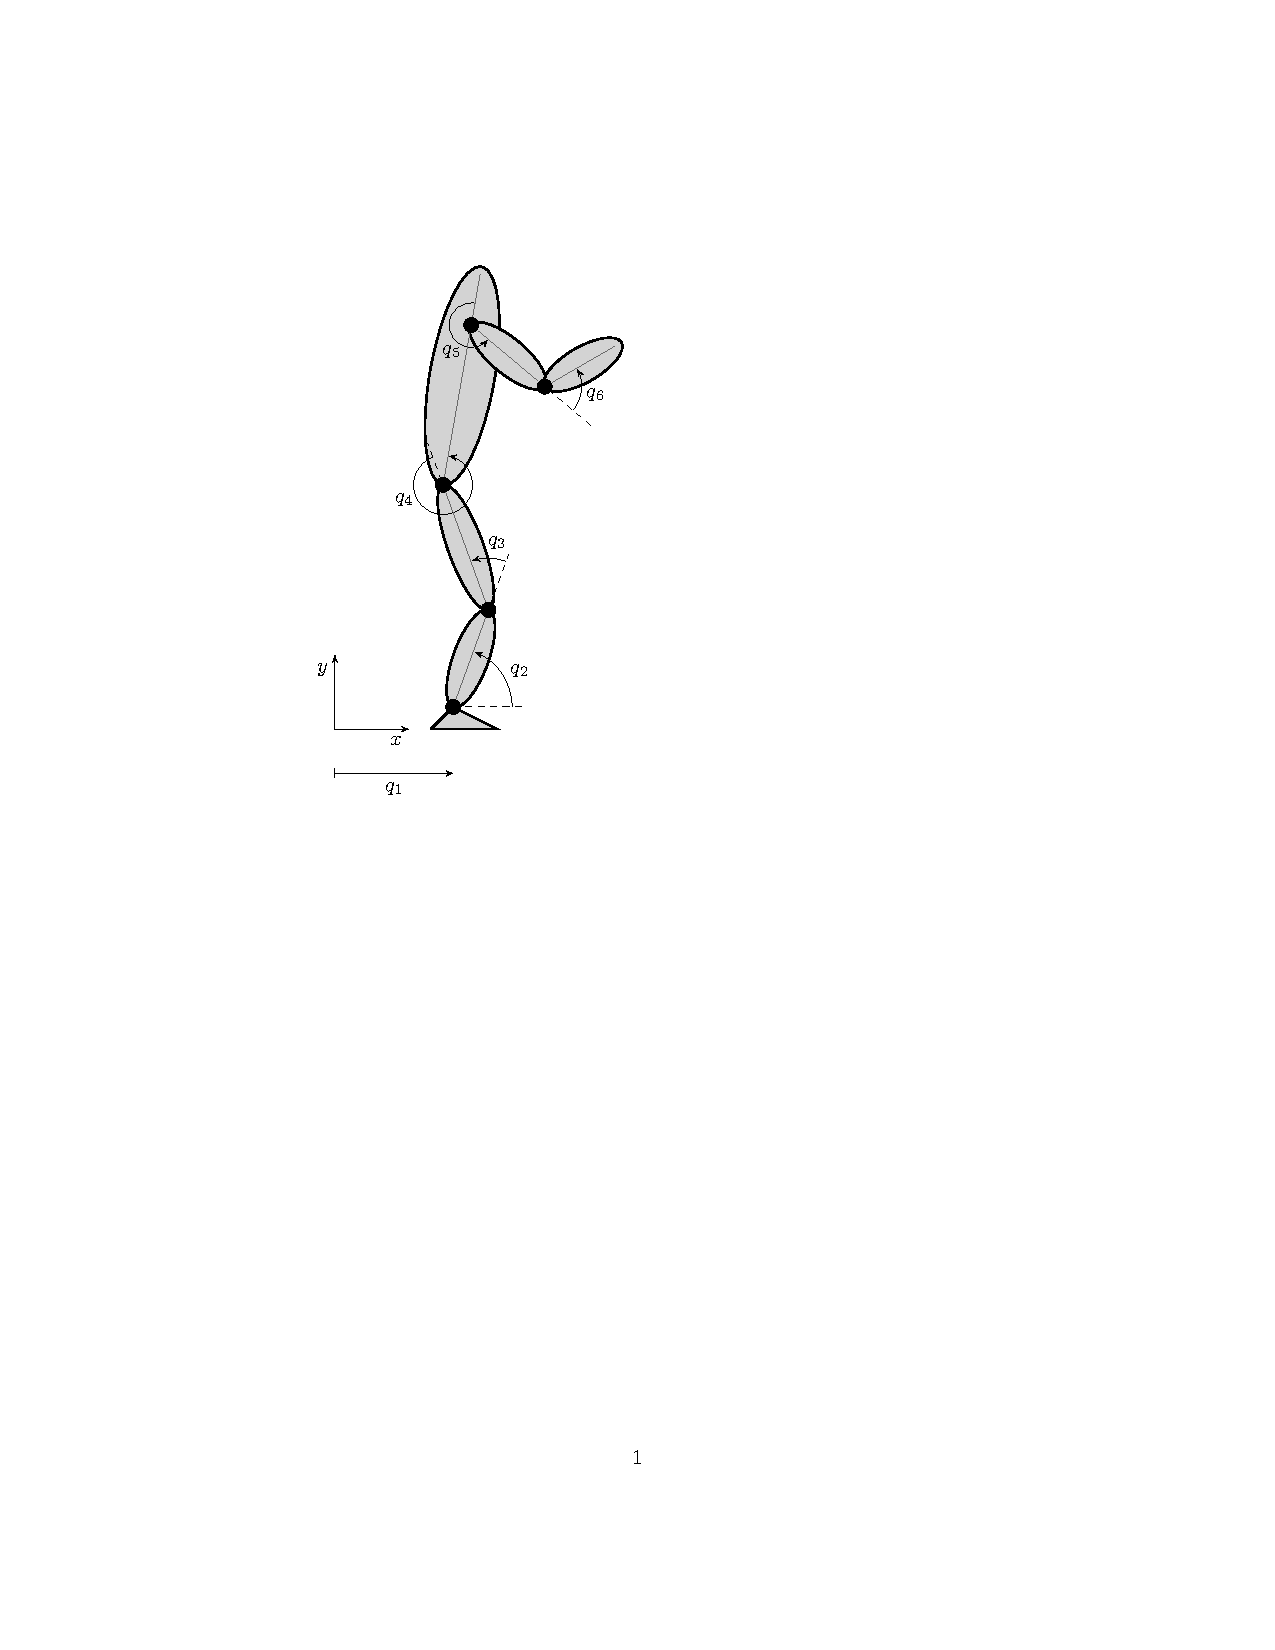
\includegraphics[trim=53mm 144mm 110mm 44mm, clip,
    scale=0.8]{images/planarhumanoid.pdf}
	\subcaption{Schematic diagram of the robot model and its coordinates}
   \label{planarhumanoid}
	\end{subfigure}
	\begin{subfigure}[b]{0.45\textwidth}
	\centering
	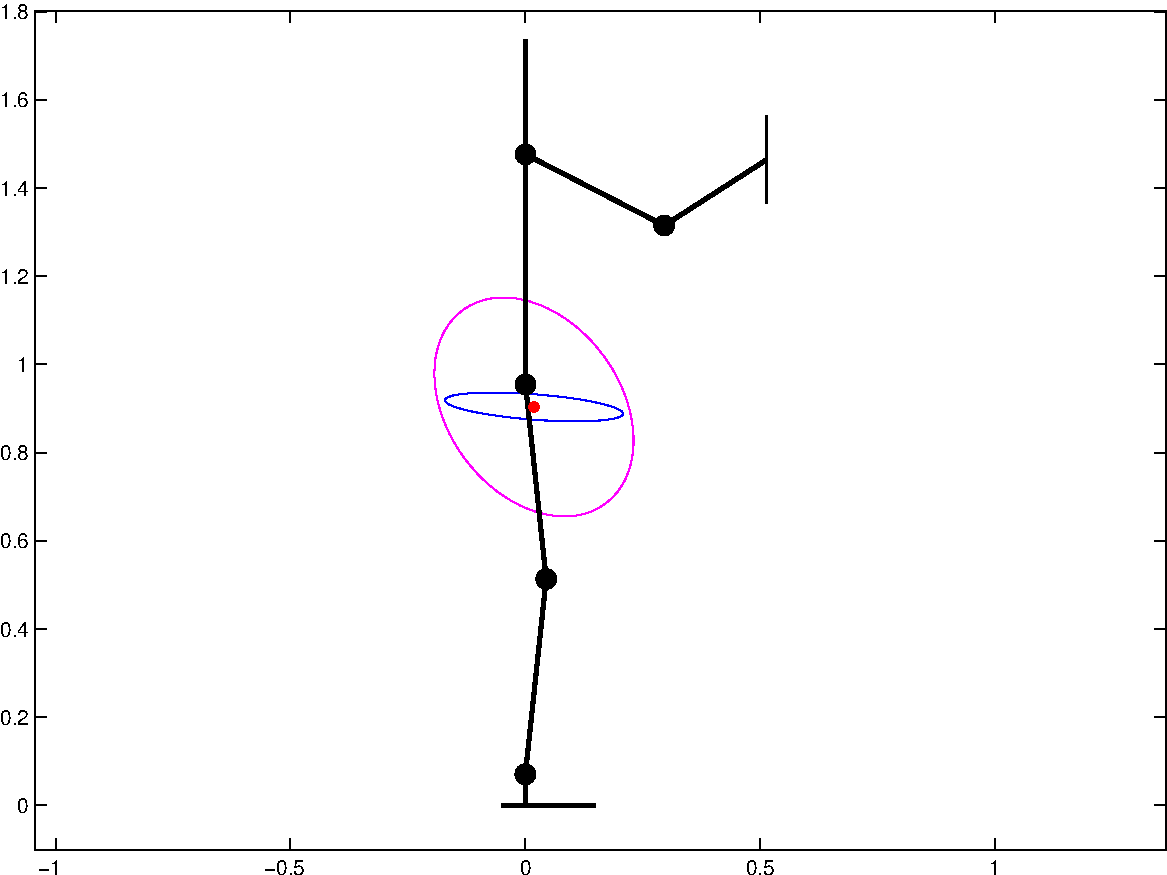
\includegraphics[trim=45mm 0mm 65mm 5mm, clip, scale=0.5]{images/ellipses.pdf}
	\caption{Velocity ellipses for a planar humanoid robot}
	\label{ellipses}
	\end{subfigure}
\end{figure}

During the second year, UB continued to work on defining a suitable metric to
measure the effects of the environmental contacts on the robot's stability.
They used the basic concept of end-effector manipulability (for manipulators)
in the literature and introduced a new tool to analyze the ability of balance
for legged robots which we called it manipulability of the center of mass.
This tool defines three different types of ellipsoids which are called 1)
velocity ellipsoid, 2) instantaneous velocity ellipsoid and 3) instantaneous
velocity ellipsoid due to the unit impulse.  The first one shows the velocity
of the CoM in different directions due to the unit norm of the joint
velocities.  The second and third types of the ellipsoids, which are obtained
by using impulsive dynamics, show instantaneous changes of the CoM velocity
due to the unit norm of instantaneous changes at the joint velocities and the
unit norm of impulse at the actuated joints, respectively.  By involving the
motion equations into the calculations for the second and third types of
ellipsoids (via impulsive dynamics), these ellipsoids allow us to study the
effect of under-actuation as well as kinematic constraints on the robot's
stability.

As an example, Fig.~\ref{ellipses} shows a planar humanoid robot (with its hand 
is fixed) and instantaneous velocity ellipses for the robot in the
specified configuration. Since the robot is fully actuated, the first and
second types of ellipses (type 2 and type 3) are the same. This ellipse (type
2) shows how the velocity of the CoM changes when the instantaneous change of
the joint velocities due to the impulse has the unit norm. This shows the
ability to move the CoM in different directions by a certain amount of
movements at the actuated joints. The ellipse type 3 shows how the velocity
of the CoM changes due to the unit impulse at the joints. In other words, it
shows how a certain amount of impulse at the actuated joints can accelerate
the CoM in different directions. All of the ellipses are independent from the
controller and they are dependent only on the physical parameters of the robot
and its kinematic constraints.

In balancing in a plane, the CoM movement in the horizontal direction is an
important measure. By projecting a velocity ellipse on $x$ axis, we obtain a
line which its length equals to the maximum change of velocity of the CoM in
the horizontal direction. Figure \ref{type2} (left side) shows maximum
instantaneous change of the CoM velocity in the horizontal direction for
different constrained hand locations (i.e. different elbow and shoulder
angles). This is due to the unit norm of instantaneous change of the joint
velocities. In the right side of this figure, the graph at the left side is
compared with the case that the hand is not constrained. It is obvious that
the movement of the CoM is limited due to the kinematic constraint at the
hand.
\begin{figure}[!t]
  \centering
  \begin{tabular}{lr}
    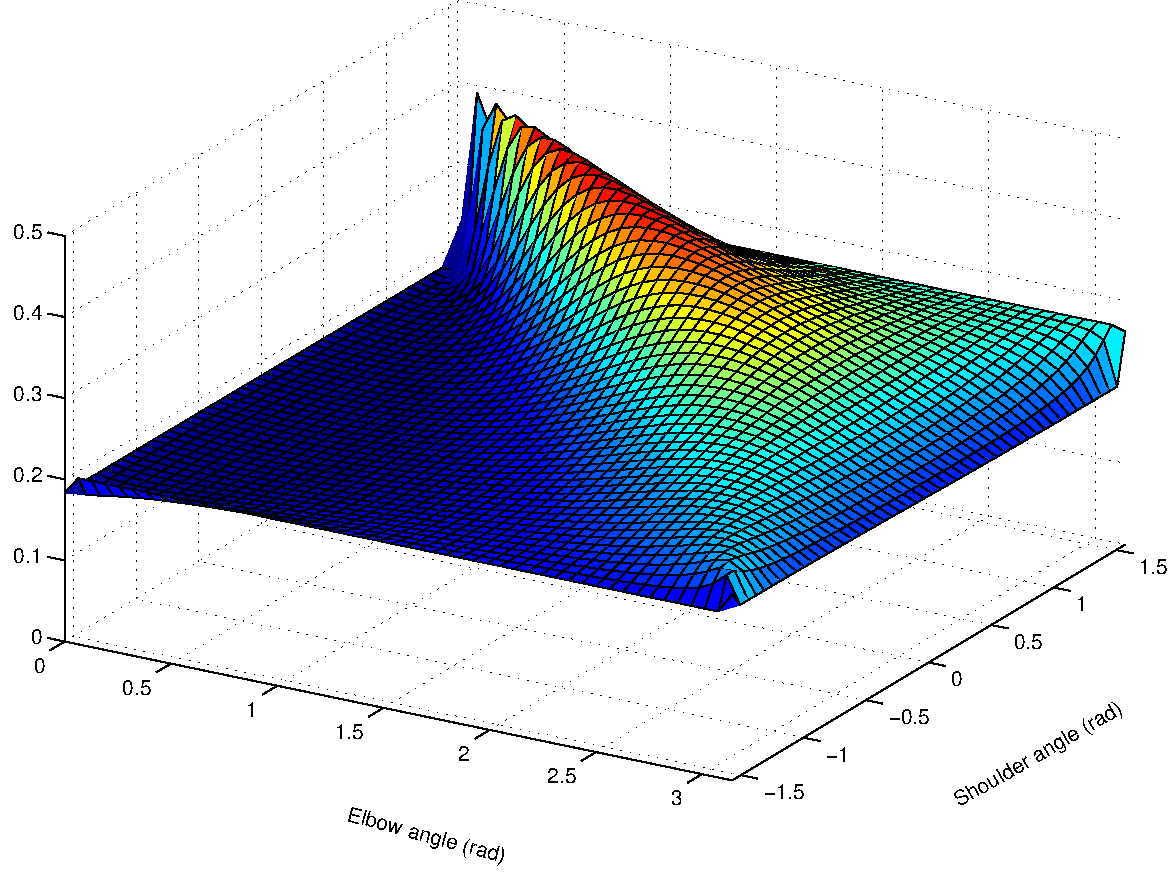
\includegraphics[width=0.5\linewidth]{images/type2_2.pdf}
    &  
    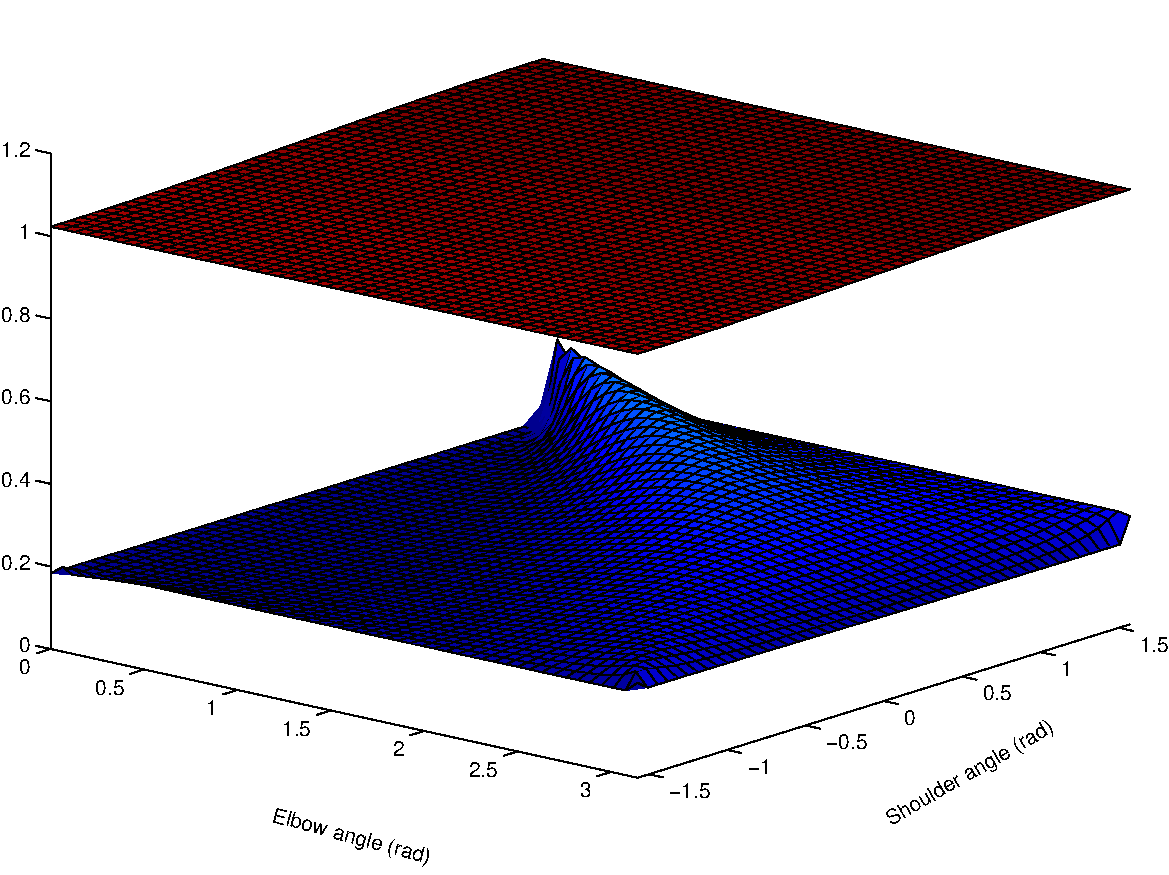
\includegraphics[width=0.5\linewidth]{images/type2.pdf}
  \end{tabular}
  \caption{Maximum instantaneous change of the CoM velocity in the $x$
    direction due to the unit norm of instantaneous change of the joint
    velocities for (left) the constrained robot and (right) for both
    constrained and unconstrained robots.}
  \label{type2}
\end{figure}

Figure \ref{type3} shows maximum instantaneous change of the CoM velocity due
to the unit impulse at the joints for different hand locations and for both
constrained and unconstrained hands. As it can be seen in this figure, the
graph for the constrained robot is always higher than the other one. This
implies that the same amount of impulse can cause bigger changes at the CoM
velocity in the constrained robot rather than the unconstrained one. The
reason is that, in the constrained case, the robot exploits the contact force
to accelerate the CoM and therefore less (impulse) torque is needed for the
same change at the CoM velocity.
\begin{figure}[!t]
  \centering
  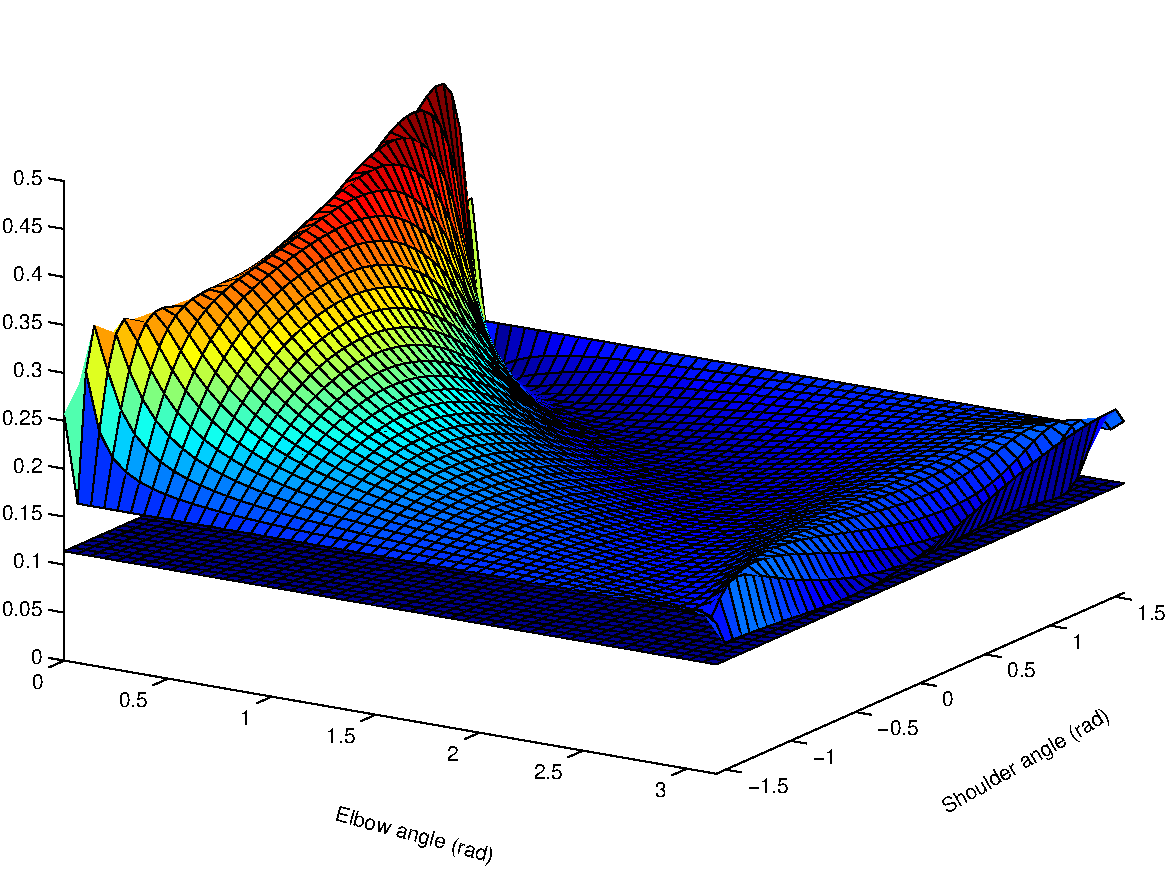
\includegraphics[width=\linewidth]{images/type3.pdf}
  \caption{Maximum instantaneous change of the CoM velocity in $x$ direction
    for the constrained and unconstrained robots due to the unit norm of
    impulse at the joints.}
  \label{type3}
\end{figure}







\subparagraph{Strategies of dealing with uncertainties in contact (T2.3)}

During the second year work on T2.3, JSI developed a novel method to study human strategies of dealing with contacts with uncertain environment. In this method the human subject was made to perform psychical contacts with the environment through the robot. The human was included into the robot control loop through human-robot interfaces. The idea is that the human sensorimotor system and cognitive system controls a novel mechanical system, i.e. the robot, in physical interaction with the environment. This implies additional human motor control learning and adaptation that can potentially provide us with a deeper insight into how humans deal with a novel environment.

Another advantage of this approach is that the human sensorimotor system does not use its own limbs to directly make the contacts with the environment, but uses the robotic limb to do so. Compared to pure biomechanical studies, where the measured human behaviour must be further interpreted, adjusted or transformed before it can be used on the robots, in this approach the measured human behaviour can be directly captured and used in the robot control. This study therefore provides a good complement to our conventional biomechanical studies as performed in T2.2.

The block scheme of the proposed approach is shown in Fig. \ref{fig:scheme}. The human controlled the motion of the robotic limb with the motion of his/her own limb. In addition to controlling the motion, the human also controlled the impedance of the robot. Primary information about the robot state was relayed to the human through a visual feedback. A haptic device was used to provide the human with an additional feedback about the forces sensed by the robot. While controlling the robot in the proposed human-in-the-loop approach, the human central nervous system had to adapt to a new mechanism through sensorimotor learning to perform the desired contact with the environment.
\begin{figure}[!t]
  \centering
  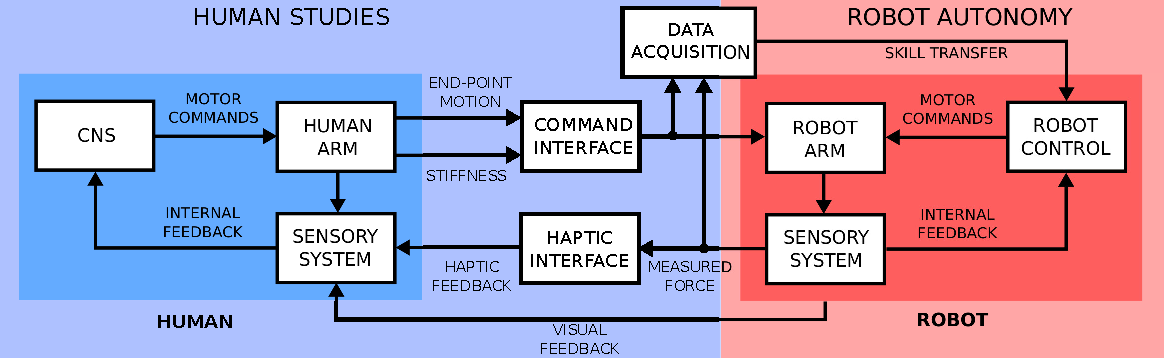
\includegraphics[width=\linewidth]{images/scheme.pdf}
  \caption{Block diagram of proposed human-in-the-loop robot control framework for study of human behaviour in contacts with environment. During the learning and adaptation stage, the human performs the contacts with the environment through the robot (blue section). The acquired data was used to observe and study the human behaviour. When the human learning process and observation is complete, the learnt skill can be directly captured and used in the autonomous robot control (red section). This is the main advantage compared to the conventional biomechanical studies.}
  \label{fig:scheme}
\end{figure}

The main goal of studies of human behaviour in contacts with environment in WP2 is to offer a basis from which we can devise equivalent humanoid robot behaviour. The most appealing prospect of the proposed approach to study human motion in contacts with the environment is that the data from the study can be used to directly form skills for autonomous robot control. The sensorimotor data was collected while the human was making the desired physical contacts with the environment though robotic mechanism. This data was then used to form the trajectories. The trajectories were encoded with Dynamical Movement Primitives (DMPs) \cite{Ijspeert2002}. The parameters of DMPs were learned by locally weighted regression \cite{Schaal1998}. The learned trajectories represented the robot skill for dealing with the contacts with the environment according to the human strategy. The trajectories can be included into the robot control system and used for autonomous execution of the learnt task.
\begin{figure}[!t]
\centering
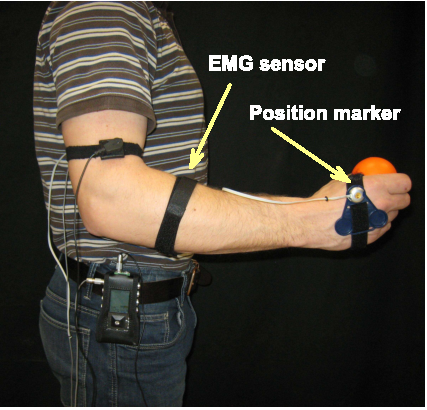
\includegraphics[height=3cm]{images/emg_setup.pdf}
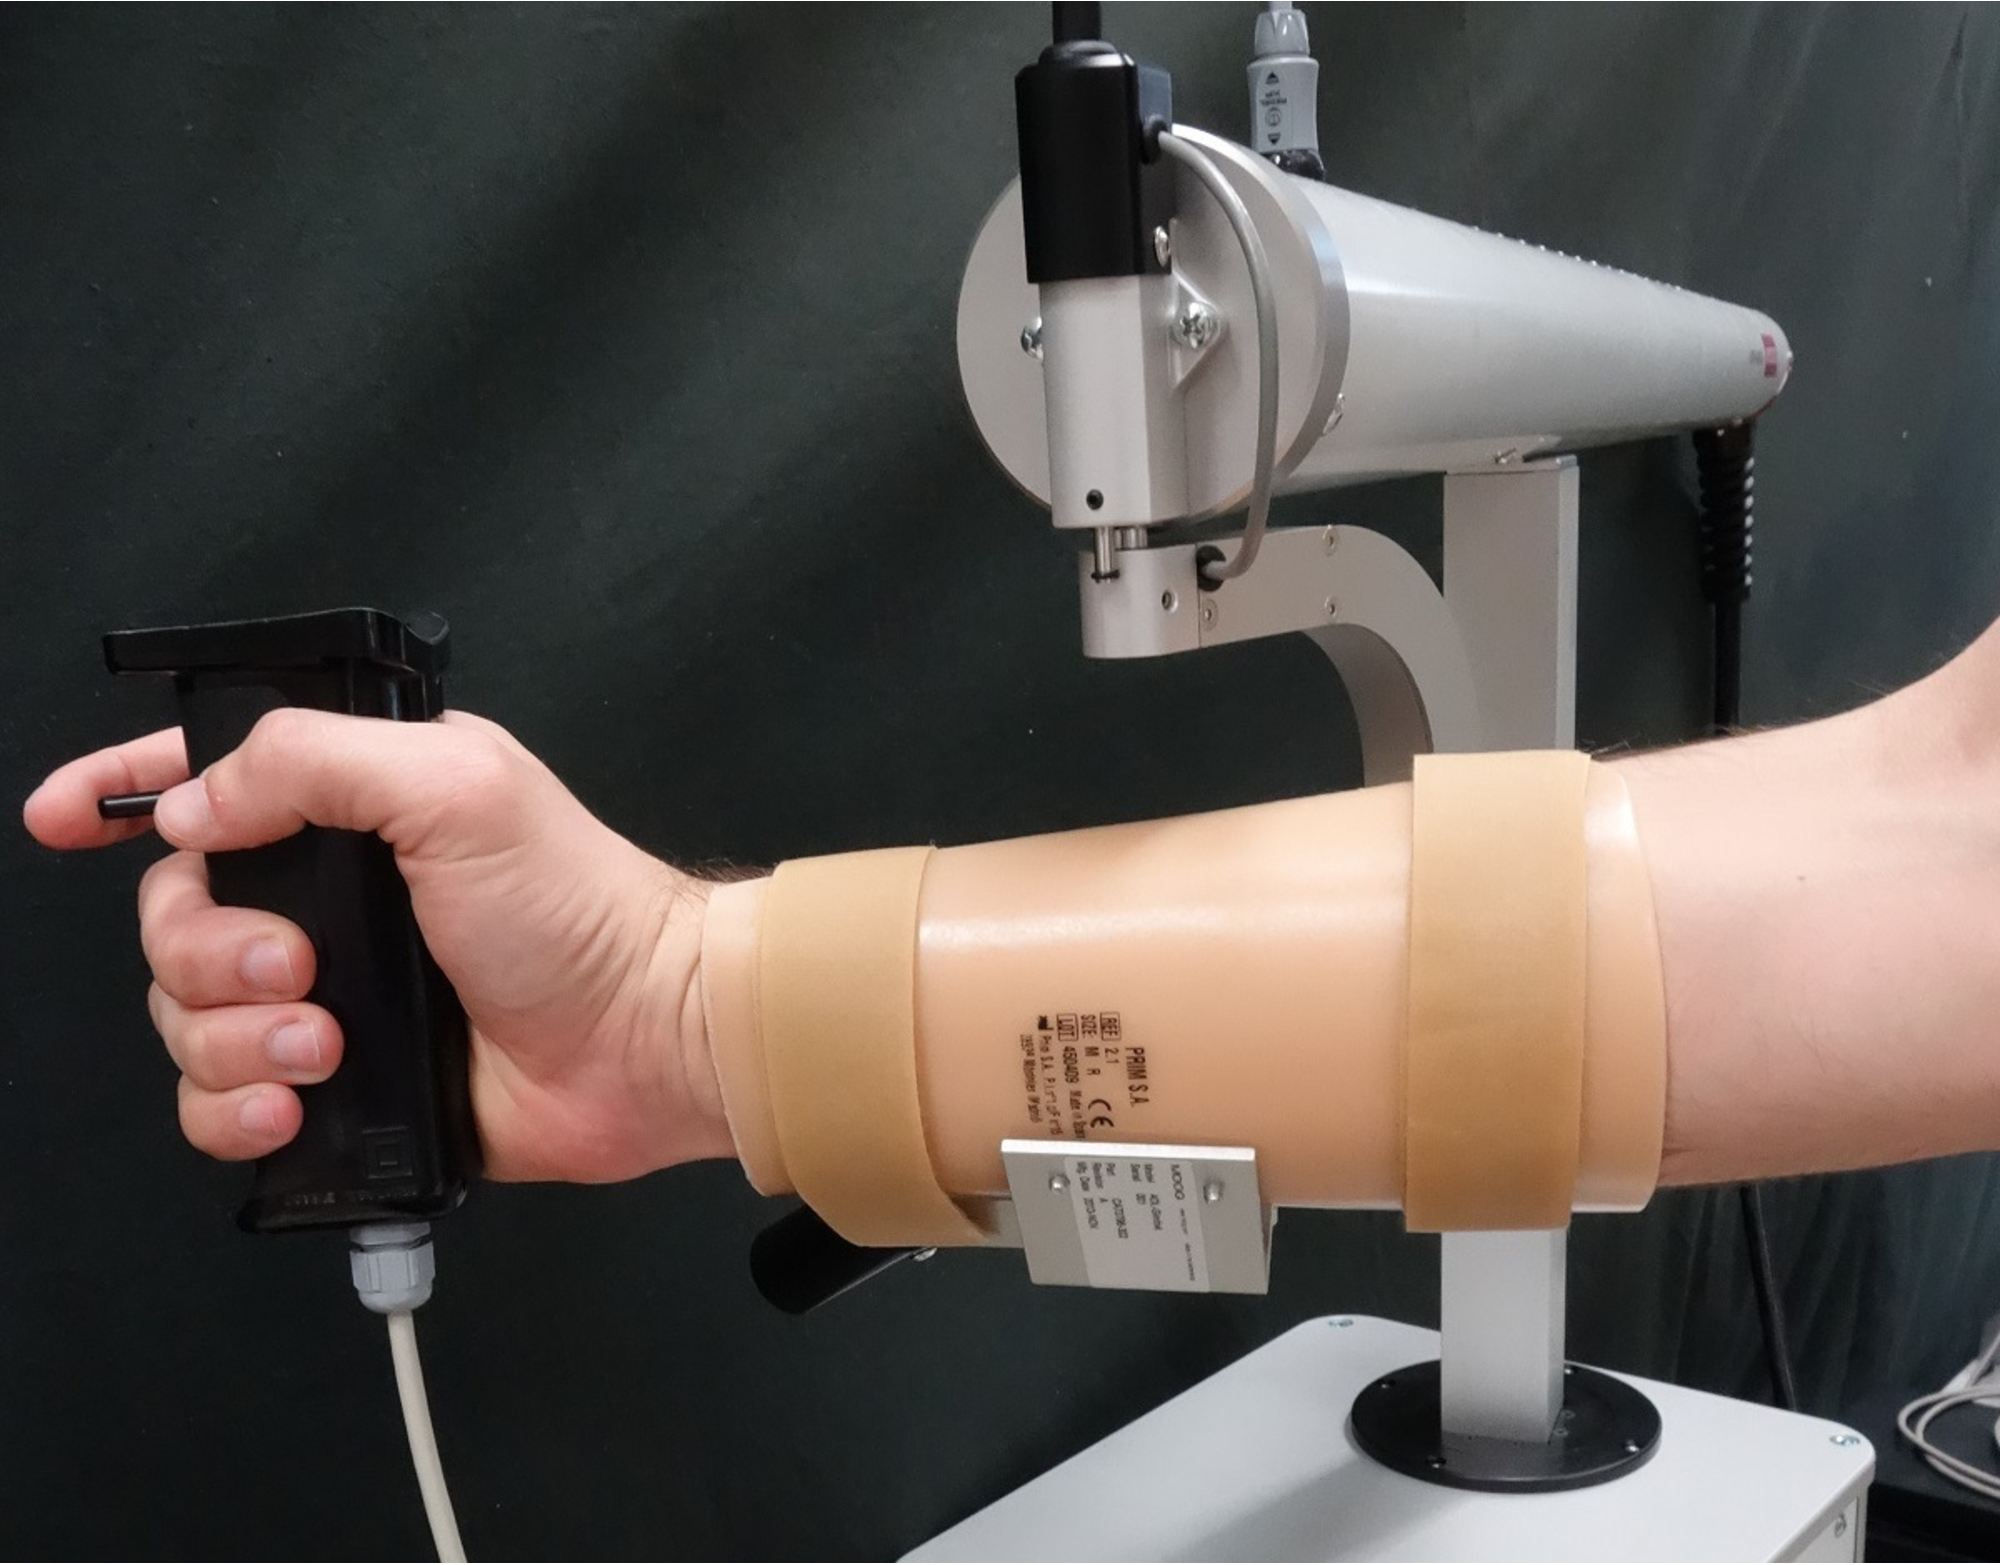
\includegraphics[height=3cm]{images/haptic.pdf}
\caption{Human-robot interfaces. First developed interface (left) measured human limb motion via optical motion capture system and mapped it to the motion of the robotic limb. The human muscle activity was measured by sEMG and was used as an interface to control the robot impedance. Second developed interface (right) consisted of \textit{HapticMaster} robot and impedance control handle. \textit{HapticMaster} robot measured the human limb position and provided the force feedback. Impedance control handle was based around a spring-return linear potentiometer and was held in the human hand.}
\label{fig:interface}
\end{figure}

One of the key features of the proposed approach is the ability of the human to directly control the impedance of the robot limb in an equivalent way that he/she controls his/her own. For this purpose we developed two novel human-robot interfaces \cite{Peternel2014,Peternel2015} that allow the human to modulate the stiffness of the robotic limb in real-time. The first interface (see Fig. \ref{fig:interface}, left) was based on measuring human muscle activity by surface electromiography (sEMG). The current measured muscle activity was mapped to the robot stiffness. The second interface (see Fig. \ref{fig:interface}, right) was based around a linear potentiometer inside a handle held in the human hand. The human controlled the position of the potentiometer knob with a finger position. The finger position is then mapped to the robot stiffness via measured potentiometer voltage.








\subparagraph{Human contact choice and learning through physical interaction (T2.4)}

Within T2.4, Inria, TUD and UPMC participated in analysing the dataset of the EDHHI experiments\footnote{\url{http://www.loria.fr/~sivaldi/edhhi.htm}} where healthy adults (18-65 years old) interact physically with the iCub (see  Fig.~\ref{fig:eddhi_picture}). The analysed data include tactile data from the forearm skin and contact forces, estimated by the iDyn modules developed in WP1. The preliminary analysis shows that people, on average, learn quickly how to interact with the robot and move its arms: across three trials, the exchanged forces are smaller and the contacts more precise. Currently, Inria is coupling the analysis of tactile and force signals with individual factors and social signals exchanged by the two peers.

\begin{figure}[!t]
  \centering
  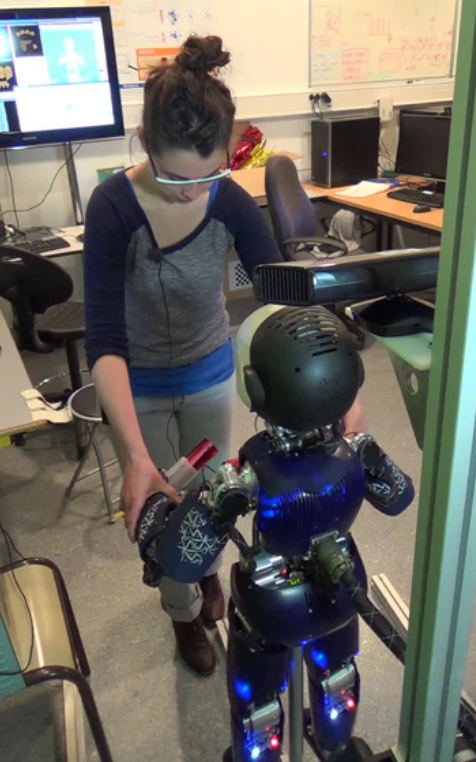
\includegraphics[width=0.48\textwidth]{images/eddhi_illustration.png}
  \caption{View of a physical interaction between a human and the iCub robot.}
  \label{fig:eddhi_picture}
\end{figure}

In the scope of T2.4, JSI studied how additional hand contact with the surrounding objects influences whole-body balance conditions. The experiments were performed on multiple subjects where we challenged their balance. The experiments were divided into two main stages. Each stage had 15 sessions in which the subject's balance was perturbed for 5 minutes. In one stage the subjects did not use supportive hand contact. In the other stage they were holding a handle in front of them. We used a motorised wait-pull mechanism \cite{Peternel2013} to continuously perturb the balance of the standing subjects in either stage by exerting external forces on the approximate position of centre of mass. See Fig. \ref{fig:exp2_protocol} for the experimental setup.

\begin{figure}[!t]
	\begin{center}
		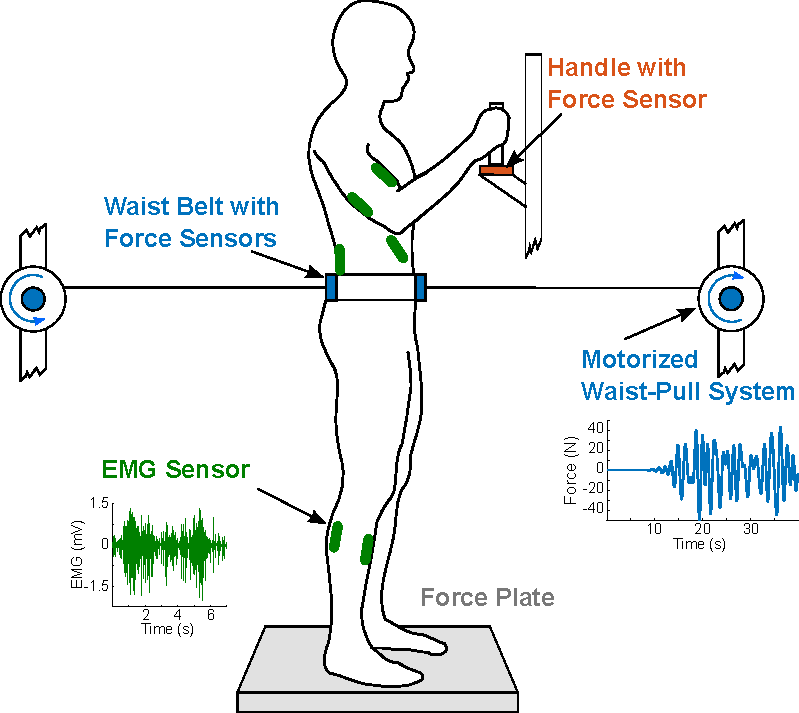
\includegraphics[width=\linewidth]{images/exp2_protocol.pdf}
		\caption{The subject was standing on a force plate, connected to the motorised waist-pull system that generated translational perturbations. The subject was holding the handle with a built-in force sensor mounted on a vertical pole. EMG electrodes were positioned on the major body muscles of the subject's right-hand side.}
		\label{fig:exp2_protocol}
	\end{center}
\end{figure}

The perturbation waveform of the waist-pull mechanism was constructed in a way that the possible muscle reactions associated with reflexes were eliminated. These reactions could potentially mask the actual role of the hand muscles as the reflex would activate the muscles unrelated to the magnitude of the perturbation. To avoid that, the perturbation waveform was continuous, had relatively low frequency and low pulling forces. During the experiment, we measured muscle activation of the subject's lower leg, trunk and arm muscles, forces in the handle and the anteroposterior movement of CoP (CoP$_{AP}$).

The results of muscle activation analysis showed that when the subjects were holding to the handle, the activation of the leg muscles was minimal (see Fig. \ref{fig:representativePSD}). Based on this we can conclude that the subjects mainly used their arm muscles to maintain postural stability. The trunk flexor muscle (Obliques Externus, OE) was more active in the stage when the subjects were holding the handle compared to when they were not. This indicates that a synergy between the arm and trunk muscles was established when additional hand contact was utilised to maintain the equilibrium.

\begin{figure}[!t]
	\begin{center}
		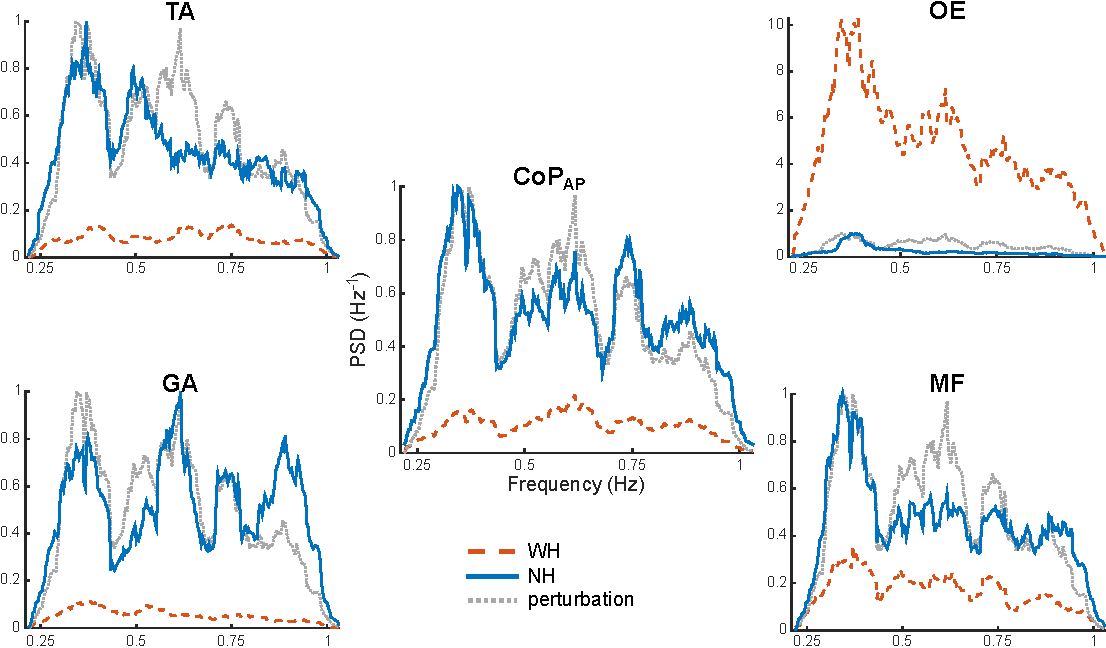
\includegraphics[width=\linewidth]{images/representativePSD_oneYaxis-v1.pdf}
		\caption{Effect of holding a handle after adaptation stabilised in the last session. The graphs show representative power spectral density (PSD) profiles of CoP$_{AP}$ and muscle activations measured in trunk and lower leg muscles. After the adaptation, effect of additional supportive hand contact stabilised to the perturbation in the last session. All EMG and CoP$_{AP}$ values are presented in a frequency domain, ranging from 0.25 Hz - 1 Hz. The blue (solid) lines represent the power in no-handle and the orange (dashed) lines in handle stage. The grey (dotted) line is the power of the perturbation signal. All signals are normalized to the peak value in the last session. The effect of handle is shown as reduced muscle activation in all muscles in the handle session, except in the trunk flexor muscle (OE), where there is an opposite effect.}
		\label{fig:representativePSD}
	\end{center}
\end{figure}

The analysis of the CoP$_{AP}$ movement showed that the displacement of the CoP$_{AP}$ was progressively dropping throughout the repeated sessions of the experiment (see Fig. \ref{fig:COPapAndTau}). This was true both in case when supportive hand contact was used and in case when no supportive hand contact was used. These results give a strong hint that a learning and adaptation was present through the sessions of the experiment, as the subject gradually improved the balance control.

\begin{figure}[!t]
	\begin{center}
		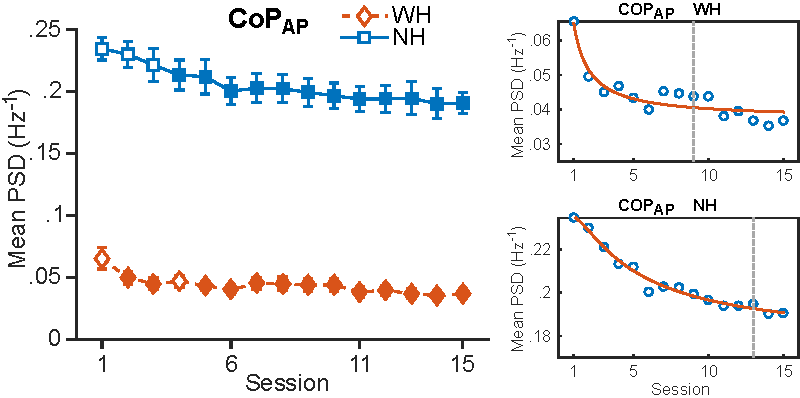
\includegraphics[width=\linewidth]{images/COPapAndTau.pdf}
		\caption{Adaptation of movement of CoP$_{AP}$ is shown on the left graph. Experimental stage with handle (WH) is shown in red, while condition without handle (NH) is shown in blue. Full markers indicate statistically significant differences between the first session and each of the following sessions. In both stages the adaptation is statistically confirmed (\textit{p} < .001). In the stage where the subjects were holding the handle, the adaptation appeared right after the first session. In no-holding stage it appeared after the third session. The superimposed best-fit curves are shown on the right graphs with orange solid lines. A calculated session number at 3$\tau$ of the fitted curve (vertical dotted line) indicates faster stabilisation of adaptation in the handle stage, compared to no-handle stage.}
		\label{fig:COPapAndTau}
	\end{center}
\end{figure}

We further analysed whether there are any effects of repeated sessions on adaptation of muscle activation and movement of CoP$_{AP}$ (Figure \ref{fig:meanErrorBars}), and whether there are any differences between the two stages of the experiment. The results show that the effect of human adaptation in lower leg muscles was statistically significant in the stage when the subjects were not using the additional hand support. However, this was not the case for the stage when the subjects were holding to the handle.

The activation of the trunk extensor muscle (MF) was almost the same in both stages and throughout all sessions. On the other hand, the activation of the trunk flexor OE remained unchanged throughout the sessions only in the stage when subjects held the handle. The activation of OE was much higher in this stage compared to stage when subject did not use supportive hand contact.

\begin{figure}[!t]
	\begin{center}
		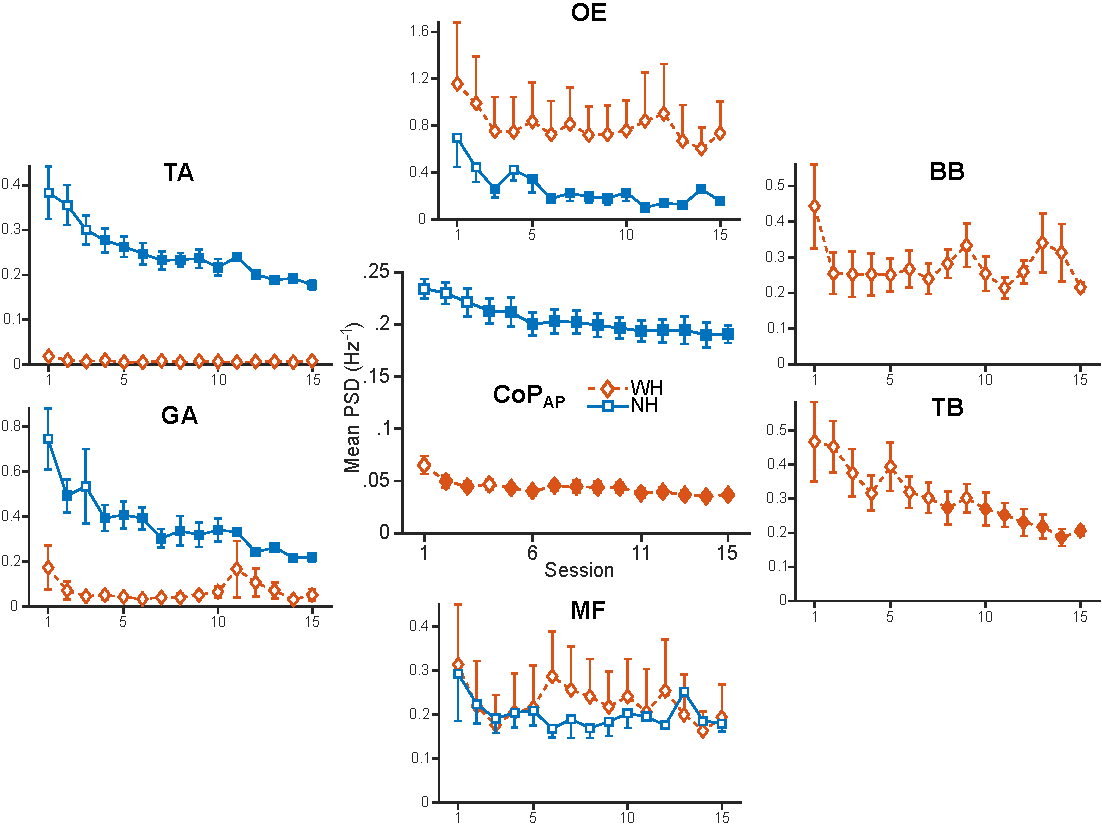
\includegraphics[width=\linewidth]{images/meanErrorBarsAll.pdf}
		\caption{Figure shows the effect of repeated sessions on muscle activation and CoP$_{AP}$ movement. Blue squares with SEM represent mean PSD in no handle and orange diamonds with SEM represent mean PSD in handle condition. Coloured markers indicate statistically significant sessions (mean values of individual session compared to the mean of the 1st session).}
		\label{fig:meanErrorBars}
	\end{center}
\end{figure}

We performed an analysis of differences in EMG activation levels between the two experimental stages in the frequency spectrum of the perturbation waveform (low = 0.25 - 0.5 Hz, medium = 0.5 - 0.75 Hz, high = 0.75 - 1.0 Hz). A paired samples analysis between the two stage for low, medium and high frequency range revealed that there was an influence of additional hand contact on both lower leg muscles. There were confirmed statistically significant differences between the two stages in all frequency ranges and for all sessions. For the MF muscle these differences were not significant in any of the frequency range nor session. However, there were significant differences between the two stages for the OE muscle. These differences occurred in the medium and high frequency range but only in the last session.

When the subjects were holding to the handle, we recorded the forces exerted on the handle during the continuous postural perturbations. Statistical analysis of handle forces revealed that the repetition of sessions had no significant effects (see Fig. \ref{fig:HandleForces}). Even though the activation of arm extensor muscle changed (decreased) during sessions, there was no significant change in forces applied on the handle.

\begin{figure}[!t]
	\begin{center}
		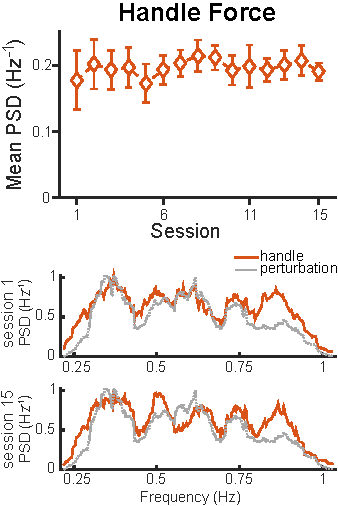
\includegraphics[width=\linewidth]{images/HandleForce-all.pdf}
		\caption{The picture shows the handle force as recorded during the proposed experiments (see text).}
		\label{fig:HandleForces}
	\end{center}
\end{figure}


\begin{figure}
\centering
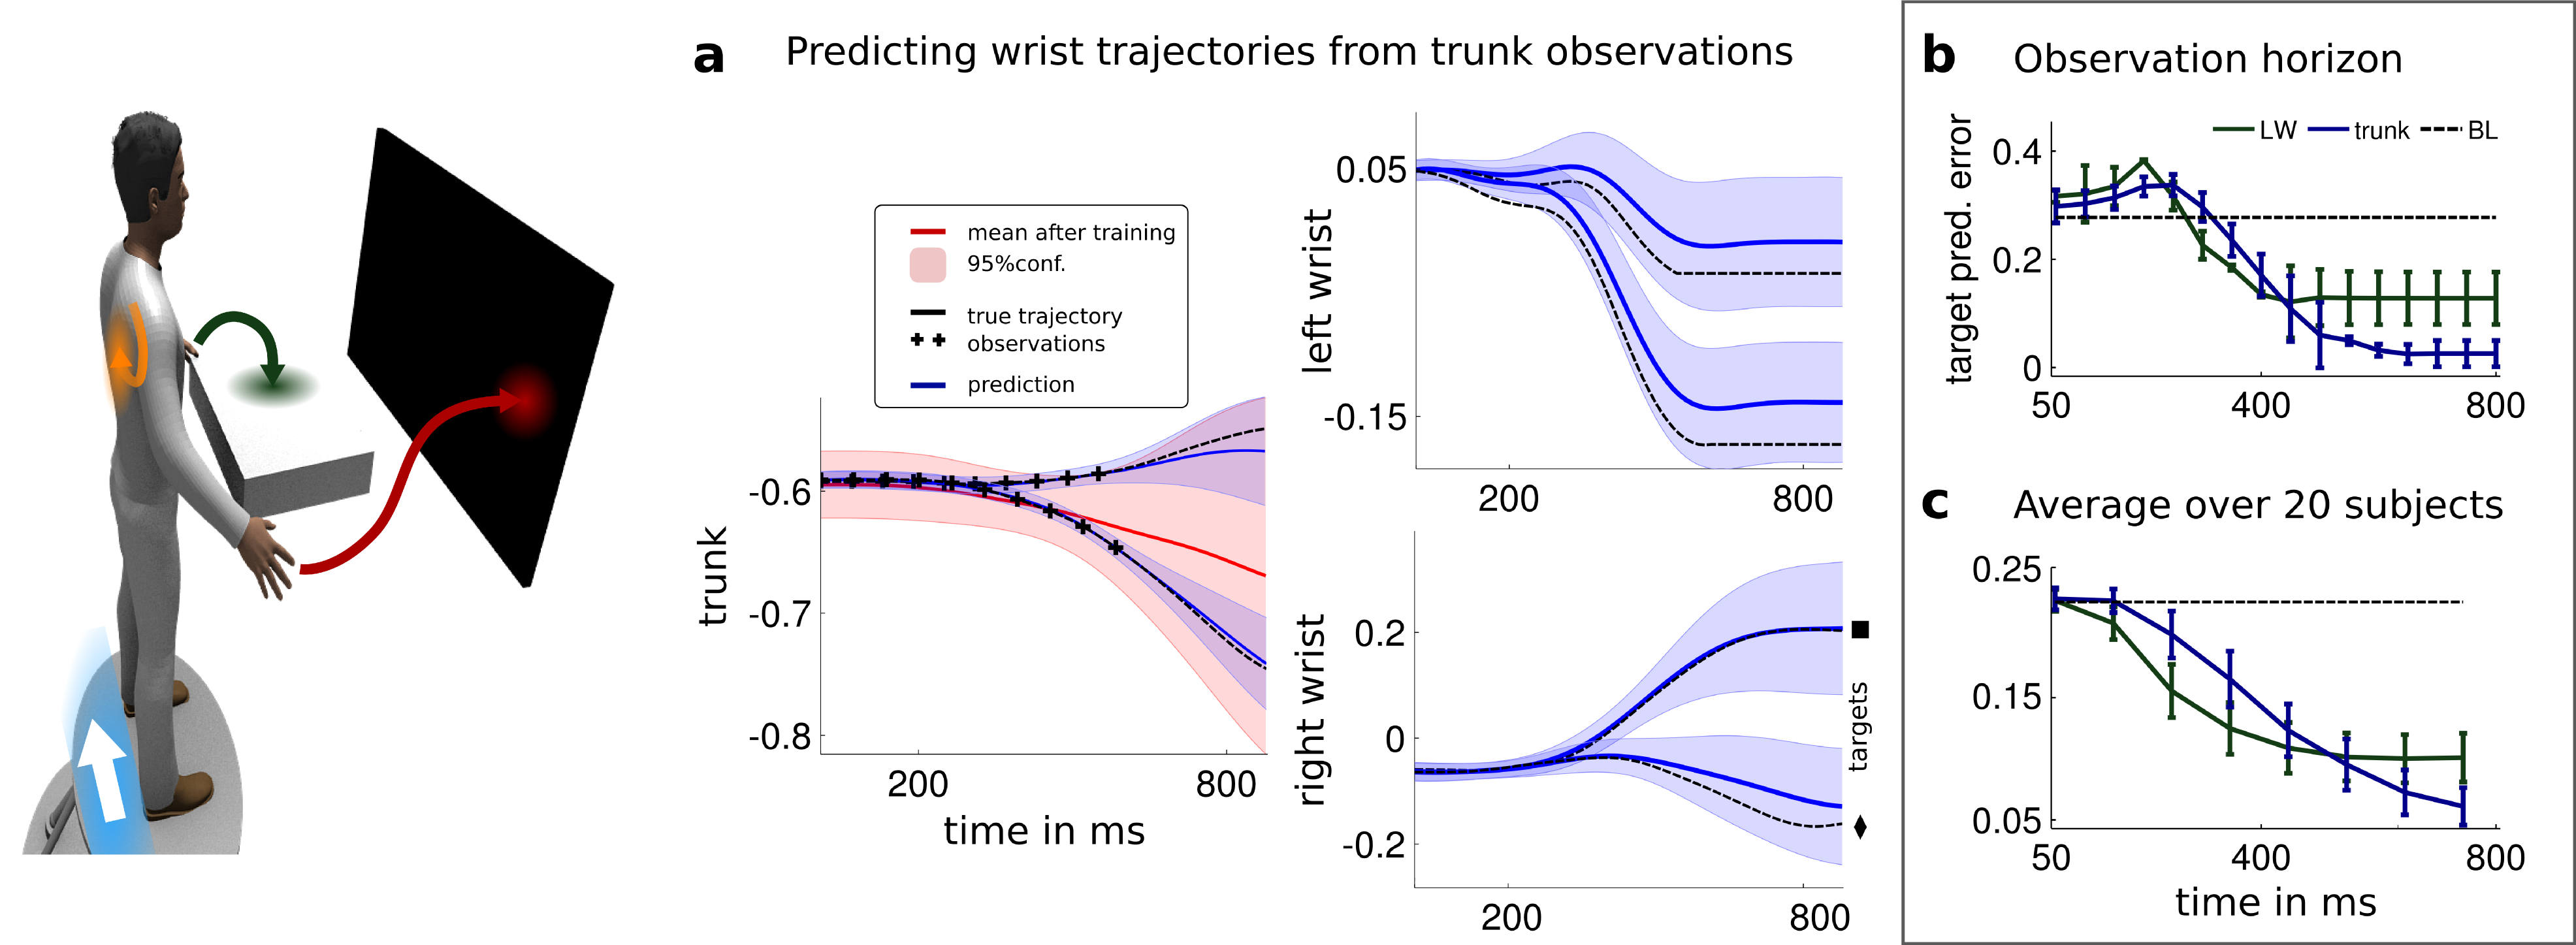
\includegraphics[width=\linewidth]{images/SummaryFig_Y2Report.png}
\caption{Trunk trajectories predict wrist trajectories. (a) 600ms of trunk trajectories are observed. These observations can predict the wrist trajectories. Shown are predictions for the two exterior targets on the screen. For training 10 trials for each target are used starting from trial 240 backwards in time (before the catch trials). For testing the first perturbed trial after trial number 240 were used. (b) The effect of the observation horizon on the target prediction error is shown for a representative subject. The mean of the training data denotes the base line (BL). (c) Average statistics (mean and 95 percent confidence bound) over 20 subjects.
}
\label{fig:HumanProMPsPrediction}
\end{figure}

In collaboration with JSI, TUD studied whether supporting contacts in human arm reaching tasks are planned or an effect of a reactive controller. Investigations on human motor learning has focused on adaptation experiments with fixed contact points leaving research on the computational role of contacts as a free control variable unexplored.

In perturbed target reaching experiments sketched in Figure \ref{fig:HumanProMPsPrediction}, we studied weather supporting contacts are planned or reactive. Subjects had to reach for distant targets on a screen with their right hand. For reaching the target additional support through contacts with a table using the left hand was inevitably. If the contacts are planned then the left hand's motion can predict the right hand reaching.

We studied how probabilistic inference in learnt models can be used to answer this question. Evidence for planned contacts could be provided through learning probabilistic models of trajectory distributions and using the models to generate predictions, Figure \ref{fig:HumanProMPsPrediction} (a). We found that the target on the screen could be predicted from both, the left hand (mse: $10.4$cm $\pm$ $2$cm over $20$ subjects) and the trunk movement (mse: $6.7$cm $\pm$ $1.4$cm over $20$ subjects), which is illustrated in Figure \ref{fig:HumanProMPsPrediction} (b-c). The learnt probabilistic model could also be used to analyse the rate of adaptation of the left hand and the trunk kinematics, where the trunk trajectories converged faster than the left hand motion. This is intuitively explained by the strong need for corrective trunk movements in balancing. A report on the findings is currently in progress of writing.

Driven by the question on how human CNS optimizes arm reaching motions when the supportive hand contact has to be reached in order to maintain postural balance, UPMC and JSI started a combined experimental and computational study where the aim is to challenge two well-established but conceptually separated motor control phenomena: (i) Humans tend to reach faster to a target that looks more rewarding, despite the additional muscular cost of a faster movement \cite{Fitts1954}, and (ii) when humans have to be precise, movements take longer to perform \cite{Shadmehr2010}. The aim of our study is to experimentally disclose both phenomena and evaluate a novel computational model designed to join them. We obtained several very promising preliminary results indicating a general mechanism that can unify both phenomena and point out a global trade-off arising from the interactions between movement time, cost and accuracy. The experimental setup is shown in Figure ref{fig:UnifyingTwoPhenomena} A report on the findings is currently in progress of writing.


\begin{figure}
\centering
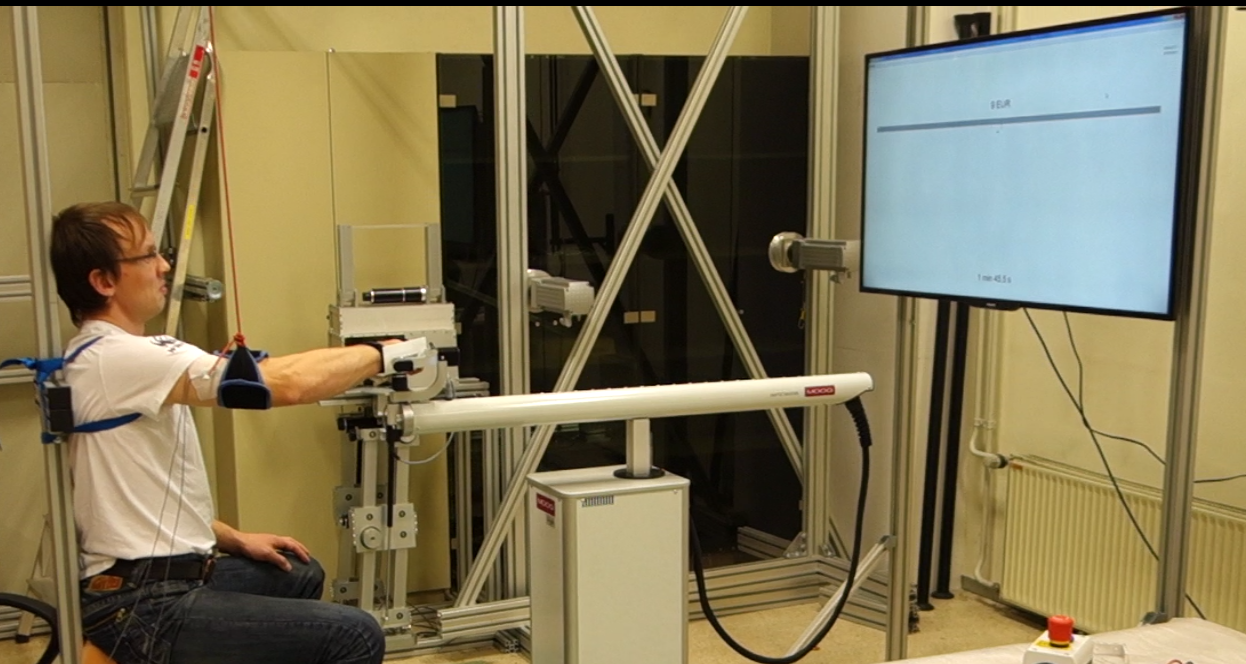
\includegraphics[width=\linewidth]{images/UnifyingTwoPhenomena.png}
\caption{Experimental setup to understand how humans optimize arm reaching motions when the supportive hand contact has to be reached in order to maintain postural balance. The task of the subject was to obtain as high reward as possible in the given time by hitting a target on the virtual wall without knowing its actual size. In effect, the subjects had to find the optimal balance between precision, speed of motion and its cost in order to maximise the reward. To amplify the effect of cost of motion, haptic robot emulated a viscous media through which the subject had to move the hand.
}
\label{fig:UnifyingTwoPhenomena}
\end{figure}





%%!TEX root = ../../secondYearReport.tex
\subparagraph{Resources}
Overall, the use of resources within WP2 was in accordance to the plans. There was a slight increase in the amount of PM for JSI due to the fact that we could not find a suitable Post-doc but hired a PhD student instead.

\begin{center}
\begin{tabular}{|C{1.5cm}|C{1.5cm}|C{1.5cm}|C{2cm}|C{2cm}|C{2cm}|C{2cm}|}
\hline
\footnotesize \textbf{WP2 person months}& \footnotesize \textbf{IIT}&\footnotesize \textbf{TUD}&\footnotesize \textbf{UPMC}& \footnotesize \textbf{UB} &\footnotesize \textbf{JSI} & \footnotesize \textbf{INRIA} \\ \hline
\footnotesize Year 1 &  0.00     & 0.00 & 0.28 & 2.64 & 18.80  &-  \\  \hline
\footnotesize Year 2 &  0.00     & 3.00 & 0.48 & 7.67 & 22.85  &-  \\  \hline
\footnotesize Partial &  0.00     & 3.00 & 0.76 & 10.31 & 41.65 & - \\ \hline \hline
\footnotesize Overall & 0.00     & 4.00 & 1.00 & 45.00 & 55.00 & 1.00 \\ \hline
\end{tabular}
\end{center}

\subparagraph{Deviations from workplan} 
No significant deviations.

%!TEX root = ../../secondYearReport.tex
 
\paragraph{Work package 3 progress}

The progress for each task is described hereafter.

\subparagraph{Formulating the control problem (T3.2) (UPMC: 3PM)}

During Year 2, UPMC has explored the different possible usage of the Generalized Hierarchical Controller developed in Year 1 \cite{LiuGHC} and allowing the specification of both strict and soft hierarchical control problems. In \cite{LiuAutRobSpecIssue}, a quasi-static version of this controller is used in simulation for a standing scenario where the iCub robot is using an additional contact which is switched from one hand to the other. This control architecture has also been successfully applied on a KUKA LWR robot \cite{LiuICRA2015}. Tasks performances for three conflicting tasks are illustrated on Figure~\ref{fig:KUKA_LWR_GHC}.

\begin{figure}[h!]
\centering
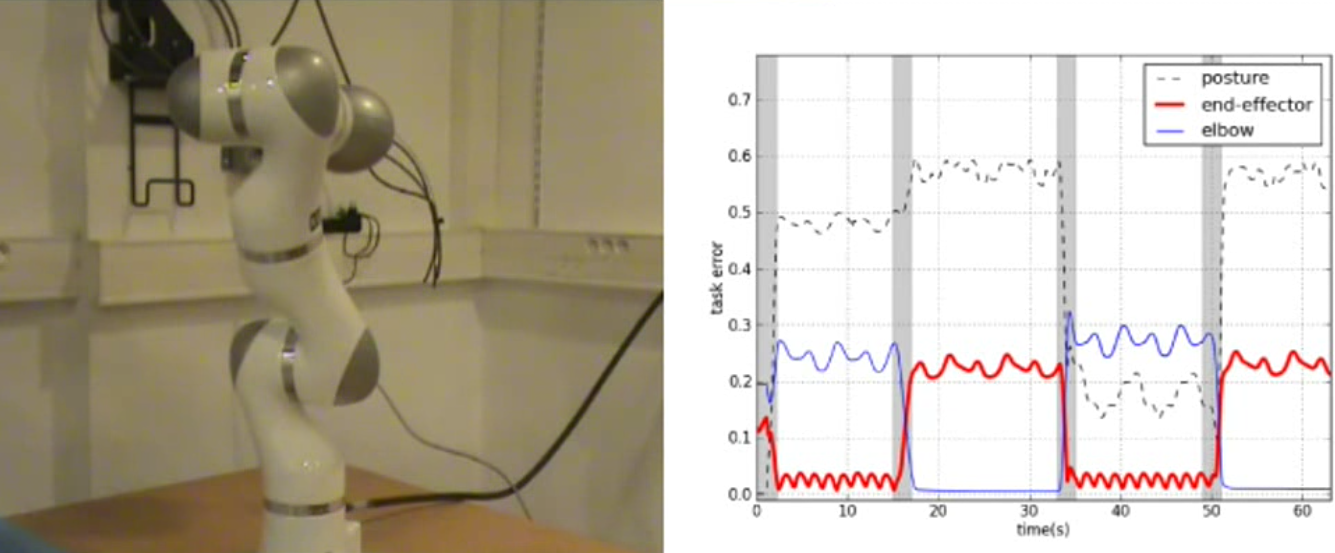
\includegraphics[width=\linewidth]{images/KUKA_GHC_ICRA}
\caption{Tasks performance for three conflicting tasks using the GHC control framework.}
\label{fig:KUKA_LWR_GHC}
\end{figure}

\subparagraph{Solving the local control problem (T3.3) (UPMC: 4.5PM, UB: 0.9PM, TUD: 2.5PM)}

During Year 2, UPMC has started to investigate scenarios where the robot is interacting with the environment through rigid and non-rigid contacts. Assuming that no information is a priori available regarding the nature of the contact surface, a first control strategy has been proposed in \cite{LiuIROS2015} where the desired contact force is adapted online as a function of the velocity of the contact point. Indeed, the risk with an unknown contact surface is to assume that it will almost instantaneously provide the required contact force to maintain the robot balance. If the surface is non-rigid, the contact point will actually move while being pushed and stable support forces will only be provided to the robot once the contact is properly established. The goal of the adaptation of the desired value for the contact force is to accelerate the obtainment of a stable contact force supporting the robot. The desired trajectory for the center of mass of the robot is also adapted to account for the non-rigidity of the contact surface. One of the advantages of this approach is that it does not actually requires the knowledge of the contact surface impedance. Figure~\ref{fig:LIU_IROS_2015} provides a view of the types of considered scenarii and the structure of the considered controller. In this work, the local control problem is solved using the solver described in \cite{salini2012} rather than the one developed in \cite{LiuGHC}. This choice is related to the fact that the computation cost of the GHC approach remains important and is too high to be actually used in a real-time reactive control architecture for a humanoid robot.\\

\begin{figure}[h!]
\centering
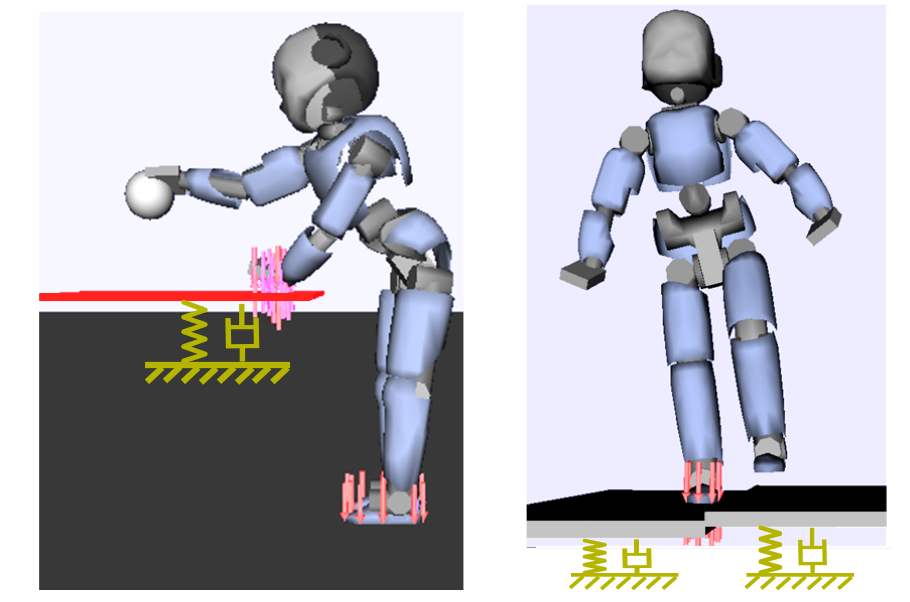
\includegraphics[width=0.45\linewidth]{images/LIU_IROS_2015} 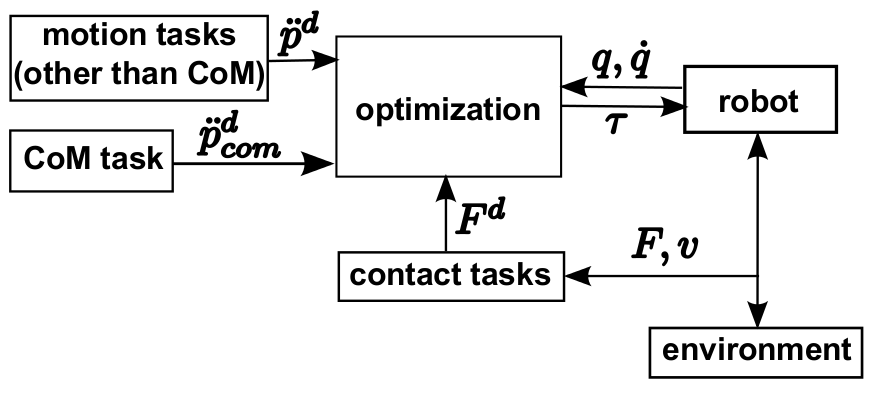
\includegraphics[width=0.45\linewidth]{images/LIU_IROS_2015_bis}
\caption{Scenarri of interaction with a non-rigid environment (\textit{left}). Structure of the adaptive control architecture (\textit{right}).}
\label{fig:LIU_IROS_2015}
\end{figure}

In the meantime, UB proposed an algorithm for implementing a momentum
based controller to control balancing motion of legged robots with non-rigid
contacts with the environments \cite{Azad&Mistry15}.  The proposed strategy
converts the balance problem to a linear constrained optimization problem
which its output is the vector of desired joint accelerations.  It first
calculates the desired supporting forces at the contact points by using the
robot’s momentum.  Then, based on the contact model and by using the Jacobian
of the contact points, it converts the desired contact forces to the desired
joint accelerations.  At the end, by using the inverse dynamics of the robot,
the joint torques are calculated.  To implement the proposed method in
practice, stiffness and damping coefficients of the contact model have to be
estimated beforehand by using contact model parameter estimation methods.\\
    
In order to best use the whole-body controllers developed within the framework of WP3, TUD hired a student for setting up the iCub hardware and simulation environment.


\subparagraph{Bootstrapping and validating the control approach in rigid world and compliant cases (T3.4) (UPMC: 7.19PM, UB: 0.95PM, TUD: 8PM, JSI: 0PM, Inria: 4PM)}

During Year 2, the whole-body controller developed by UPMC and originally described in \cite{salini2012} has been ported, using the Whole Body Interface described in Deliverable~D1.2, on the iCub robot. A non-free-floating first implementation was performed during the \textit{Veni, Vidi, Vici} 2014 summer school. The free-floating version is less straightforward as it requires: a well calibrated torque low-level control loop and a proper on-line estimation of the state of the root-body in order to  compute the dynamics and kinematics models of the robot\footnote{The retained solution is to choose one body in contact with the fixed environment as the root-body (one foot for example) and switch the root-body whenever there is a switch in the contact state of the system.}. IIT is working on these two topics and UPMC, in coordination with IIT, is pursuing integration on its iCub robots.

UPMC also kept exploring the contribution of MPC approaches to  handle the postural balancing under varying contact conditions. The contributions in this domain are related to the thesis work of A. Ibanez \cite{ibanezIROS2014} and the postdoctoral work of D. Lau\footnote{A paper has been submitted to a conference with double blind reviews and cannot be explicitly referred to for obvious reasons.}.  In order to compute optimal time, duration and position of footsteps along with the center of mass trajectory of a humanoid, a novel mixed-integer model of the system is introduced in the work of A. Ibanez. The introduction of this model in a predictive control problem brings the definition of a Mixed-Integer Quadratic Program, subject to linear constraints. Simulation results demonstrate the simultaneous adaptation of the gait pattern and posture of the humanoid, in a walking activity under large disturbances, to efficiently compromise between task performance and balance. In addition, a push recovery scenario displays how, using a single balance-performance ratio, distinct behaviors of the humanoid can be specified. Results have been obtained in simulation\footnote{A video associated to this work can be found \url{http://pages.isir.upmc.fr/~padois/website/fichiers/videos/ibanez\_IROS2014.mp4}{here}.} and are being implemented on the TORO robot developed at DLR. This work is also being adapted in order to test control hypothesis to explain the behaviours observed in the experiment developed in T2.4 of WP2\footnote{This adaptation has been discussed during the visit of Jan Babic as an invited professor during November 2014 at  UPMC}. In the work of D. Lau, two simple and novel approaches to solve for 3D locomotion with multiple non-coplanar contacts are introduced. Both formulations use model predictive control to generate dynamically balanced trajectories with no restrictions on the center of mass height trajectory. The first formulation treats the balance criterion as an objective function, and solves the control problem using a sequence of alternating convex quadratic programs, while the second formulation considers the criterion as constraints to the problem, and solves a succession of convex quadratically constrained quadratic programs. Preliminary results have been obtained in a scenario where a hand contact on a vertical wall is used to improve balance. A staircase climbing scenario has also been studied.

In coordination with T4.4 in WP4, UPMC also explored ways to optimize tasks trajectories \cite{lober-HUMANOIDS2014} and the weights of tasks \cite{lobersubmittedIROS2015} in the LQP whole-body controller in order to maximize the overall control performance. More details are provided in the description of T4.4.\\

Continuing the activities which started in the first year of the project, IIT further improved the torque whole-body controller. During the second year of the project, attention was mainly on rigid contacts even if the theoretical and software development was guided and constrained by the requirements for extending the approach to non-rigid contacts. Several improvements to the controller significantly improved its performances. Improvements include in-situ force/torque sensor calibration \cite{Traversaro2015b}, inertial parameter identification \cite{Traversaro2015} and individual motor transfer function identification \cite{Nori2015a}. These improvements made possible quite challenging control tasks like the robust single foot balancing represented in Figure~\ref{fig:footBalancing}. Details of the controller will be given in a forthcoming publication.\\

\begin{figure}[h!]
\centering
{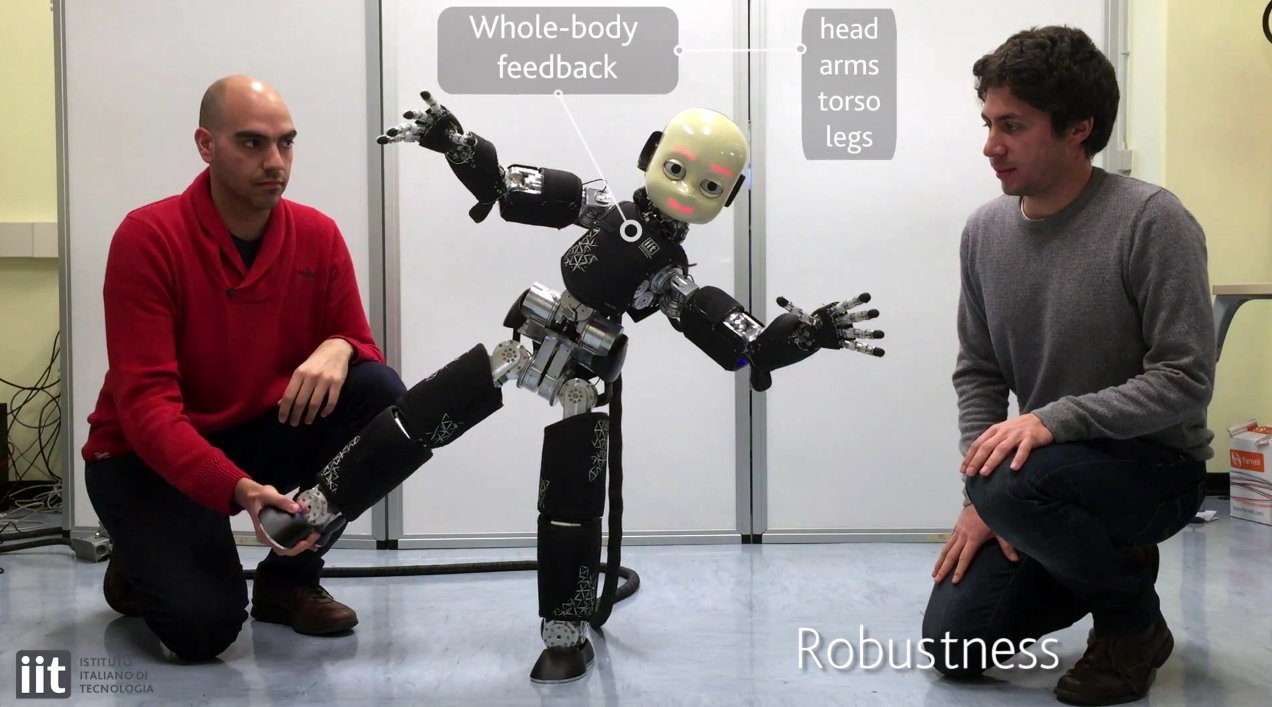
\includegraphics[width=\linewidth]{images/single_foot_balancing.jpg}}
\caption{The picture shows the iCub while performing compliant single foot balancing. Details on the controller can be found in \cite{Nori2015a}. A video of the task is available on youtube\protect\footnotemark.}
\label{fig:footBalancing}
\end{figure}

\footnotetext{\url{https://www.youtube.com/watch?v=SYVCbzGsBF4}.}


During the second year, TUD continued their research in inverse dynamics model
learning in situations with contacts. A mixture of experts approach with
Gaussian processes was developed using tactile feedback from the iCub's sensor
skin. This approach was evaluated on the iCub robot, where the learned model
accurately predicts contact forces, is robust to changes in the environment and
outperforms existing analytic dynamic models that make use of force/torque
sensor data. 
An exemplary task is illustrated in Figure~\ref{fig:exp3:icuparis_experiment_bars} 
when obstacles are introduced on both sides of a planned circular motion.
In Figure~\ref{fig:exp3:gating} can be seen that the mixture-of-experts recognize the presence of the two different contacts and opportunely active the corresponding expert to compensate for the contact.
As a result, the torques predicted from this approach (red curve) closely follow the ground truth (blue curve) and outperform the analytic model (green curve).
A paper was published in an international robotics conference
\cite{Calandra_ICRA15}. A study exploiting learned dynamics models
for control is in progress of writing. Both studies are detailed in Deliverable
D4.2.\\

	\begin{figure}[t]
		\begin{minipage}{.43\linewidth}
			\centering
			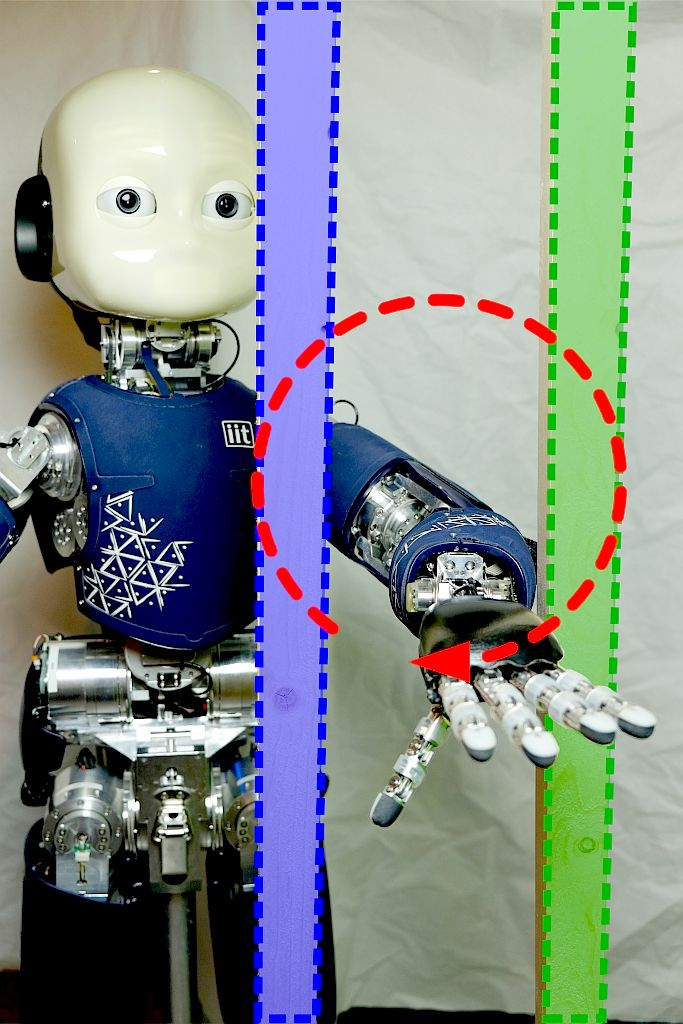
\includegraphics[width =.94\linewidth]{images/iCubParis02_Double_Contact}
			\caption{The robot performs a circle with its left arm. 
			The forearm collides alternatively with the left, the right or both contacts.}
			\label{fig:exp3:icuparis_experiment_bars}
		\end{minipage}	
		\hfill
		\begin{minipage}{.52\linewidth}
			\centering
			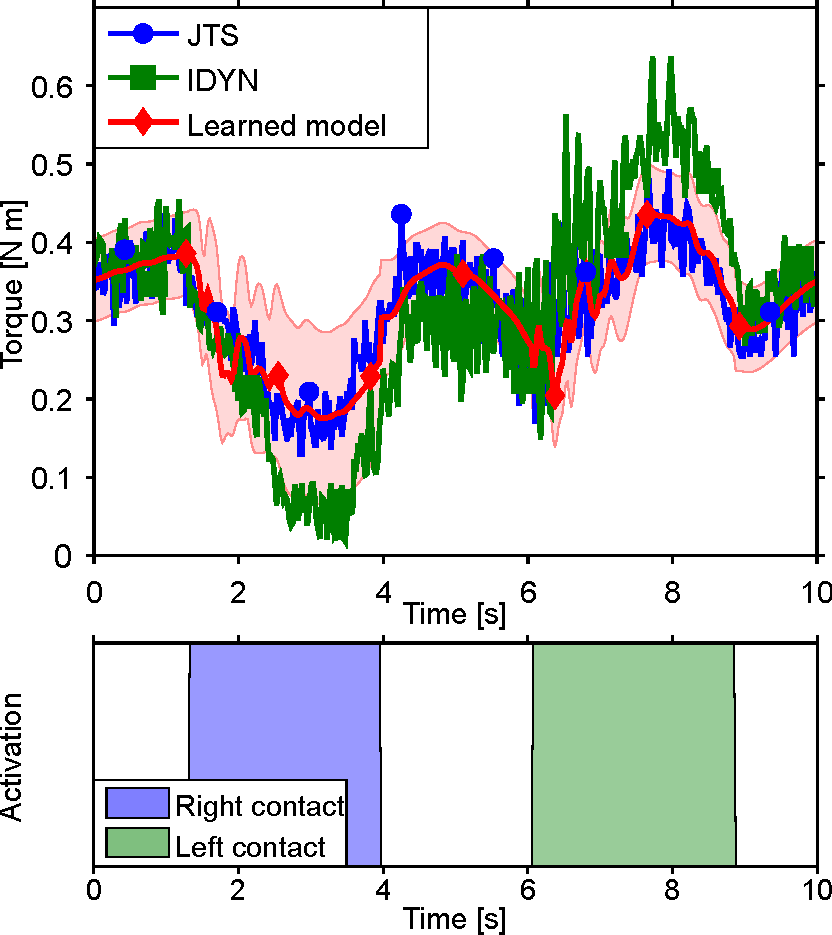
\includegraphics[width=.89\linewidth]{images/exp3_both}
			\caption{Prediction of torques with multiple contacts and the corresponding activation of the gating network.
			%Various models are shown, but individually, none of them correctly capture the dynamics of the system. 
			Our mixture-of-experts model combines the learned single-contact models into a multiple-contact model which outperform the analytic approach.
			}
			\label{fig:exp3:gating}
		\end{minipage}	
        %\figspace
	\end{figure}
	
INRIA, in collaboration with TUD, started to study the problem of bootstrapping the parameterized controllers proposed in T3.3. A major problem is how the controllers parameters, particularly the task weights, can be initialized or learned through trial-and-error. With the increasing abilities of humanoid robots, the number of tasks increases, together with their weights or priorities: manually specifying them through a sequence of complex manipulations becomes a major bottleneck. 
As a first step towards the offline optimization of those parameters, Inria evaluated the benefit of using a stochastic optimization derivative-free strategy such as \textit{Covariance Matrix Adaptation Evolution Strategy} (CMA-ES) \cite{Hansen-2001-ID362}. Figure~\ref{fig:robust} provides a view of the robustness of the optimization strategy by comparing several optimizations experiments with constant and random values for the GHC controller.
The full study is detailed in the Task 4.4.\\

\begin{figure}[h!]
  \centering
  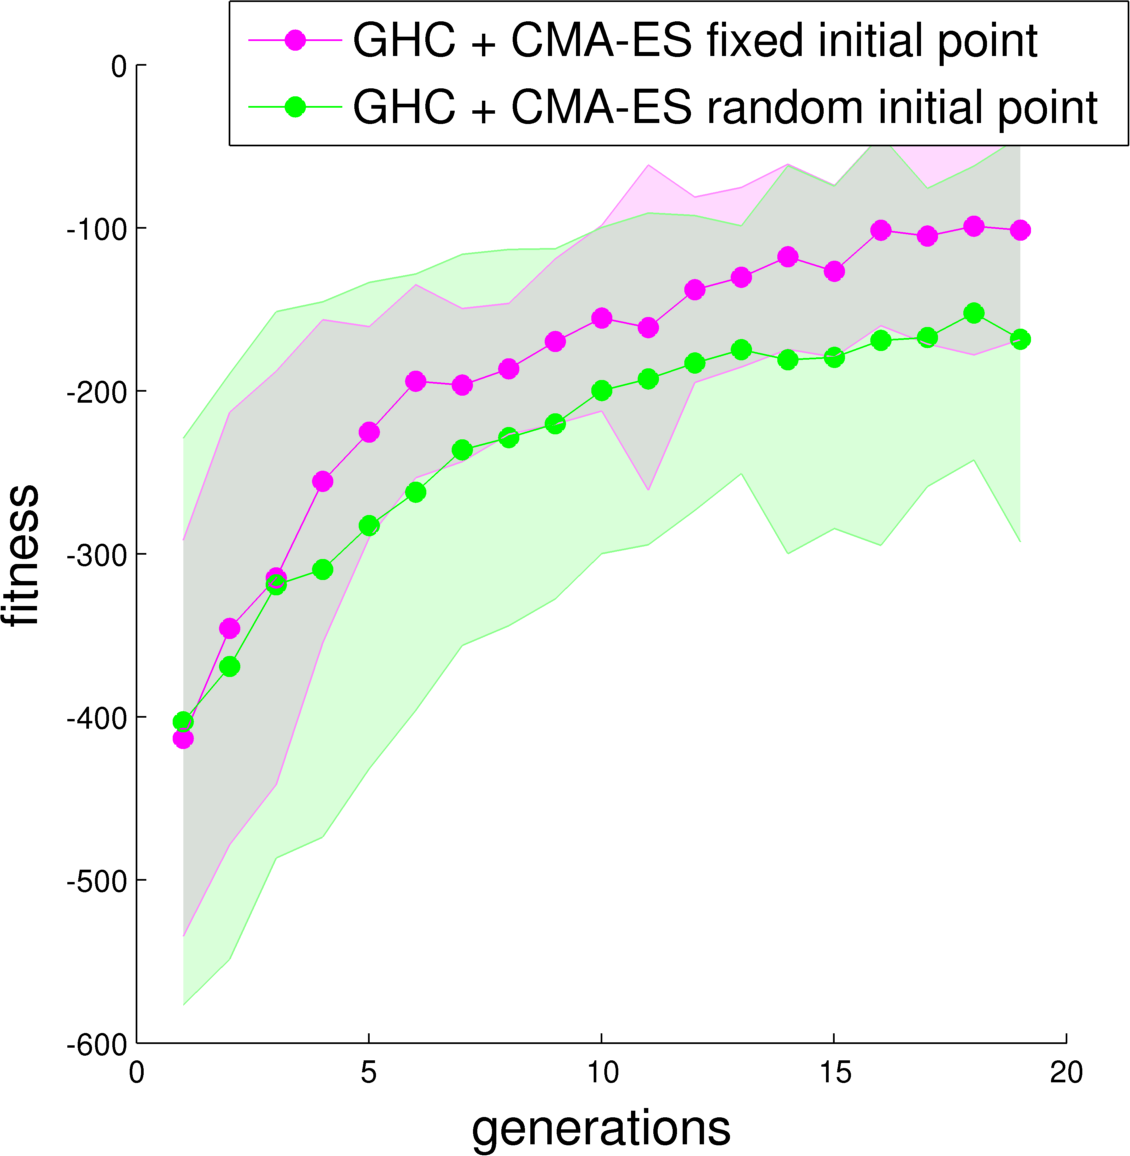
\includegraphics[width=0.5\hsize]{images/GHC_robust}
\caption{Learning the activation policies for GHC with CMA-ES. The policies were initialized with constant values $\alpha=0.5$ or random values between $[0,1]$. The mean and variance of the fitness function used for optimization for $R=20$ replicates a test experiment (see also Task 4.4).}
\label{fig:robust}
\end{figure}

In the meantime, UB also studied the problem of constrained motion for a manipulator performing
a task while in contact with the environment, and proposed a solution based on
projected operational space dynamics \cite{Ortenzietal14}.  The main
advantages of this control technique are: 1) it exploits the environment
contact constraint itself, so as to minimise the joint torques needed to
perform the task; 2) it enables full decoupling of motion and force control;
3) force feedback from a force sensor mounted at the end effector or other
contact points is not needed.  This work is a step towards a robot control
strategy which mimics the human behaviour of exploiting contacts with the
environment to help perform tasks.  They also presented an experimental
implementation of the control method in which a KUKA LWR IV manipulator used
an eraser to wipe a whiteboard.  They showed that the proposed controller can
effectively exploit contact with the whiteboard in order to reduce joint
torques while still performing the desired wiping motion.

\begin{figure}[h!]
  \centering
  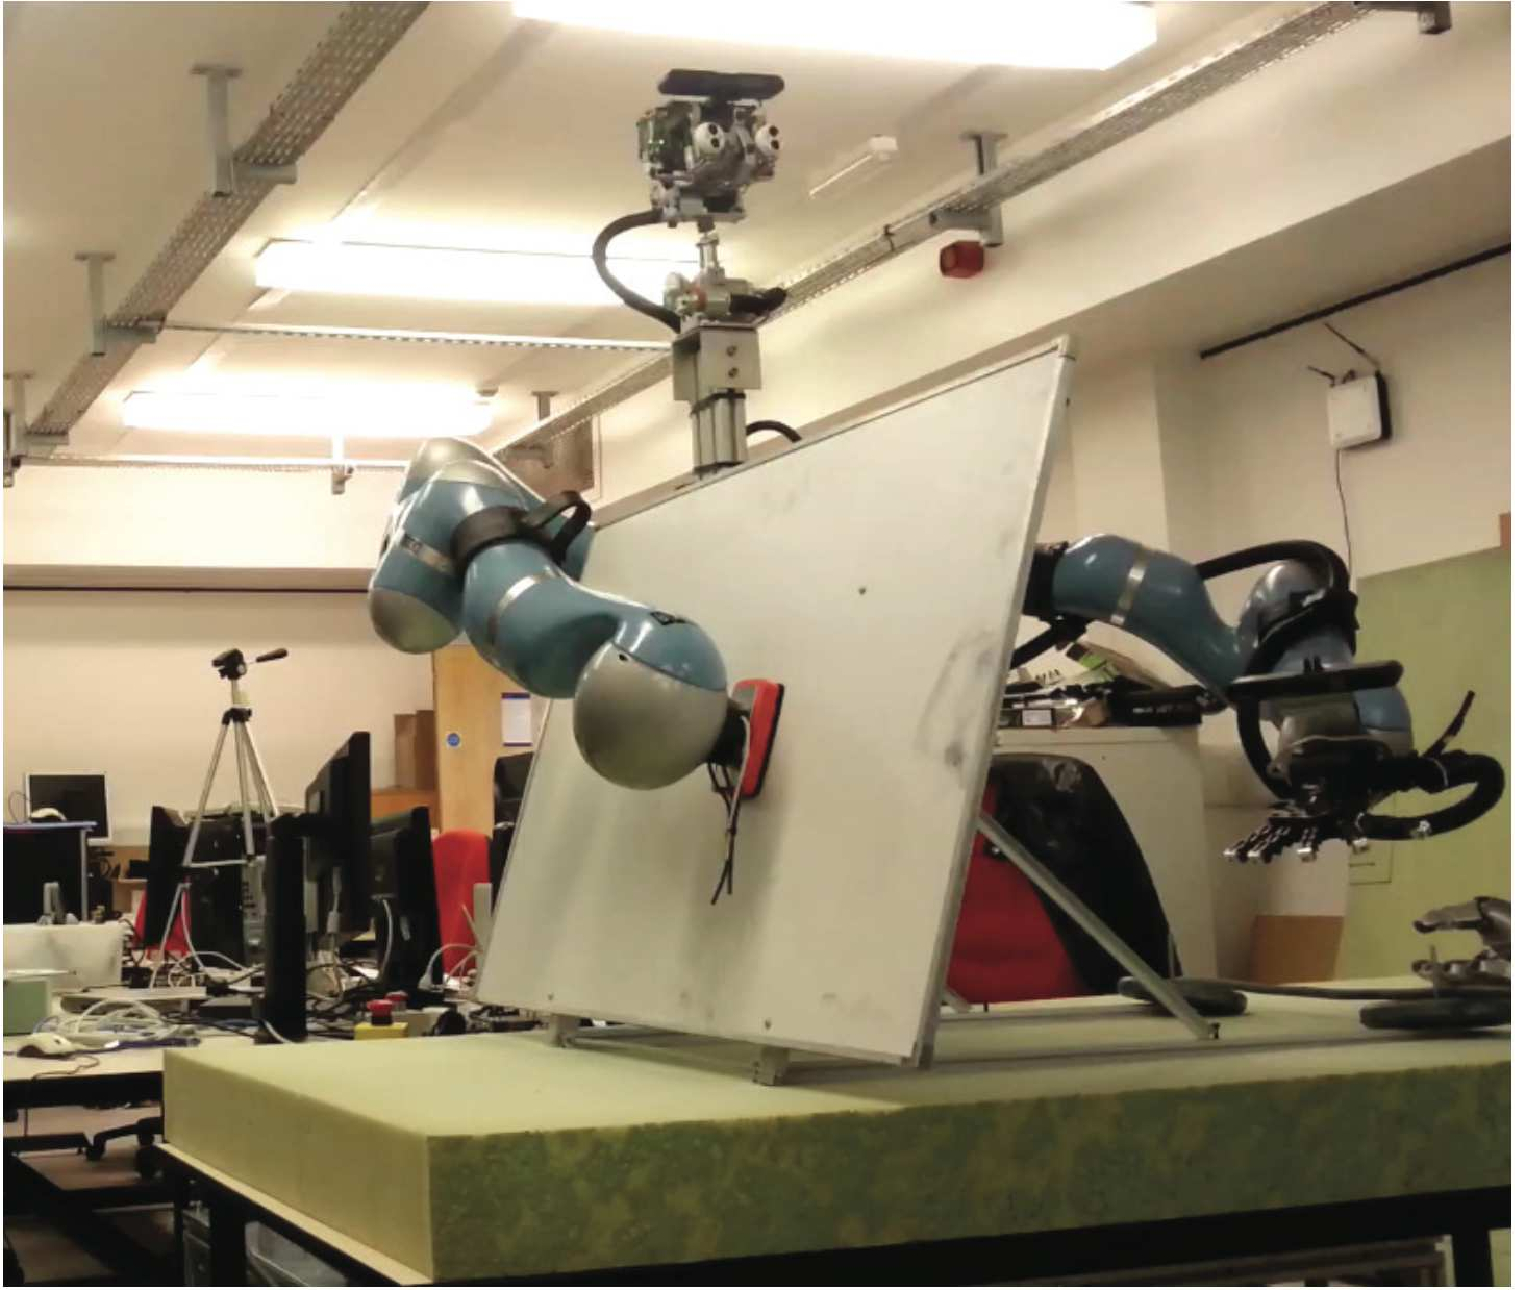
\includegraphics[width=\linewidth]{images/whiteboard.pdf}
  \caption{Experimental setting. The right arm of the humanoid
    platform Boris is used, and placed the board in between its two arms so that the z
    axis of the robot end effector frame, the z axis of the robot base frame
    and the axis orthogonal to the board are parallel.}
  \label{whiteboard}
\end{figure}










%%!TEX root = ../../secondYearReport.tex

\subparagraph{Resources}

\begin{center}
\begin{tabular}{|C{1.5cm}|C{1.5cm}|C{1.5cm}|C{2cm}|C{2cm}|C{2cm}|C{2cm}|}
\hline
\footnotesize \textbf{WP3 person months} & \footnotesize \textbf{IIT}&\footnotesize \textbf{TUD}&\footnotesize \textbf{UPMC}& \footnotesize \textbf{UB} &\footnotesize \textbf{JSI} &\footnotesize \textbf{INRIA} \\ \hline
\footnotesize Year 1 &  9.90 & 4.60 & 15.15 & 0.00 & 0.00 &  -   \\  \hline
\footnotesize Year 2 &  0.00 & 10.5 & 14.69 & 1.85 & 0.00 &  4.00  \\  \hline
\footnotesize Partial &  9.90 & 15.10 & 29.84 & 1.85 & 0.00 & 4.00 \\ \hline \hline
\footnotesize Overall &  9.00 & 24.00 & 43.5 & 10.00 & 4.00 & 10.50 \\ \hline
\end{tabular}
\end{center}

\subparagraph{Deviations from workplan} 
IIT committed own resources to WP3. In particular, Silvio Traversaro significantly contributed to T3.4 with 8PM of work with focus on whole-body parametric identification. 


%!TEX root = ../../secondYearReport.tex


\paragraph{Work package 4 progress}

\subparagraph{Improved Models from Real-Time Regression with Latent Contact Type Inference (T4.1)}%(TUD 8.5PM, ??PARTNERS)}

%IIT
Within T4.1 IIT developed a theoretical framework for estimating whole-body
dynamics from distributed multimodal sensors \cite{Nori2015}. Considered sensors
include joint encoders, gyroscopes, accelerometers and force/torque sensors.
Estimated quantities are position, velocity, acceleration and (internal and
external) wrenches on all the rigid bodies composing the robot articulated
chain. The estimation procedure consists of an extended Kalman filter (EKF)
which gives the a-posteriori estimation given all the available measurements.
Computational efficiency is obtained by formulating the Kalman filter
update-step with a sparse Bayesian network. Experiments for validating the
proposed theoretical framework have been conducted on a leg of the iCub humanoid
robot. The iCub is an ideal platform for the proposed experiment given its
distributed force, torque, linear acceleration and angular velocity sensors.
Results have shown the accuracy and the computational efficiency of the proposed
method. The theoretical framework has been implemented in an open source
software (see also Section \ref{sec:T15}).

%TUD
%LMProMPs and Model-free ProMPs
TUD extended their probabilistic movement primitive (ProMP) approach in two
ways. First, a mixture model approach that learns a shared latent structure of
related tasks from demonstrations was developed. The shared structure is encoded
by a multi-modal vector that modulates the probabilistic primitives. Both, the
probabilistic primitives as well as their activations (i.e., the latent
variable) are learned from demonstrations. In a table tennis ball prediction
tasks this latent variable modulated the slope and the waviness of the ball
trajectory. In a Kuka robot arm reaching task, the approach was used to learn
bi-modal reaching trajectories that avoid an obstacle placed in front of the
robot. This work is detailed in Deliverable D4.2 and will be presented at the
IEEE conference on Robotics and Automation in May in Seattle, USA
\cite{Rueckert_2015}. 

In a second extension of ProMPs, TUD developed a model-free control method that
can be trained from demonstrations and generates time-varying feedback control
gains that reproduces the demonstrations. In this approach a joint distribution
over states, sensory feedback (e.g., measured joint torques or contact forces)
and controls is learned. In conditioning on the current state the next-state
control-law can be computed in closed form approximating the true forward
dynamics through local linearizations given the demonstrations. TUD evalated
this model-free ProMP method on the humanoid robot iCub in lifting objects. A
conference paper is currently under review. 


\subparagraph{Inferring the Operational Space and Appropriate Controls with Multiple Contacts (T4.2)}%(TUD 4PM, ??PARTNERS)}

%TUD
For controlling high-dimensional robots, most stochastic optimal control
algorithms use approximations of the system dynamics and of the cost function
(e.g., using linearizations and Taylor expansions). These approximations are
typically only locally correct, which might cause instabilities in the greedy
policy updates, lead to oscillations or the algorithms diverge. To overcome
these drawbacks, TUD added a regularization term to the cost function that punishes
large policy update steps in the trajectory optimization procedure. TUD applied
this concept to the Approximate Inference Control method (AICO), where the
resulting algorithm guarantees convergence for uninformative initial solutions
without complex hand-tuning of learning rates. 

\begin{figure}[t]
  \begin{center}
  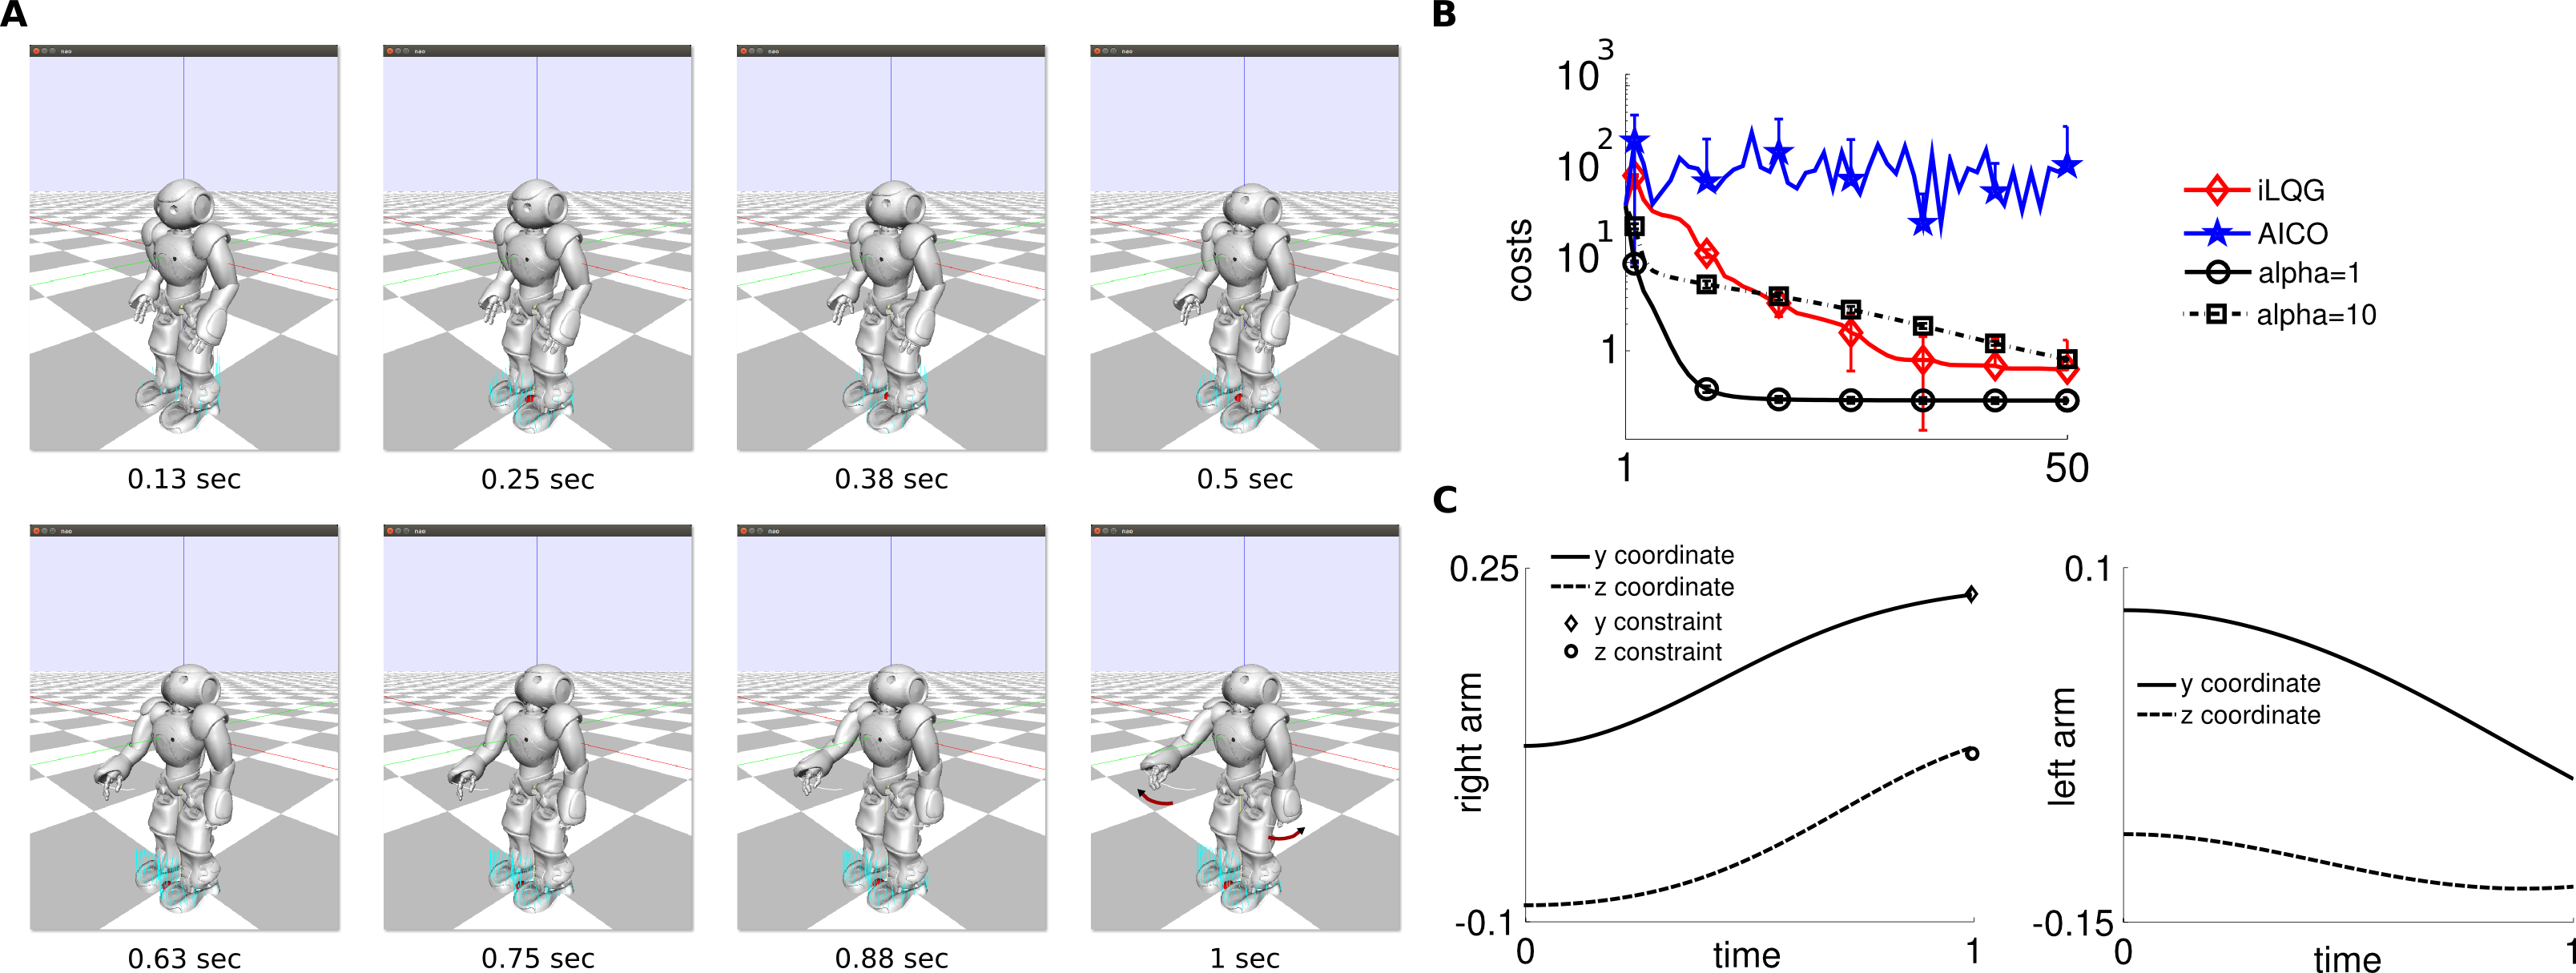
\includegraphics[width=\linewidth]{./sections/WP4/pics_elmar/NaoReachingTask.png}
  \end{center}
  \caption{Reaching task with the humanoid robot \textit{Nao}. The robot has to
reach  a desired end effector position with the right arm while maintaining
balance. Eight snapshots of the inferred movement are shown in (A). In (B), the
convergence of the costs of the optimization procedure is shown, where we
compare \textit{iLQG}, the standard implementation of AICO and the regularized
variant. The movement objectives for the right arm are shown in the left panel
in (C). To balance the robot lifts its left hand and bends the head back.}
  \label{fig:naoReachingTask}
  \end{figure}

The new algorithm was evaluated on
two simulated robotic platforms. A robot arm with five joints was used for
reaching multiple targets while keeping the roll angle constant. On the humanoid
robot Nao, we show how complex skills like reaching (see Figure \ref{fig:naoReachingTask}) and balancing can be
inferred from desired center of gravity or end effector coordinates. This work was published at 
the international conference on humanoid robots \cite{Rueckert2014}. 
Supplemental Matlab demo code is available online at http://www.ausy.tu-darmstadt.de/Team/ElmarRueckert.

\subparagraph{Generalizing and Improving Elementary Tasks with Contacts (T4.3)}%(TUD 6PM, ??PARTNERS)}

The advent of robots in our every day life can only be accomplished with
reliable mechanisms for movement generation.  Movement Primitives (MP) are a
well-established approach for representing modular and re-usable robot movement
generators that can be composed into complex movements.  An easy-to-learn
representation of the primitive is, additionally, the key of recent imitation
and reinforcement learning successes. Current MPs approaches offer viable
properties such as concise representations of the inherently continuous and
high dimensional space of robot movements, generalization capabilities to novel
situations, temporal modulation of the primitive, sequencing of primitives,
coupling between the degrees of freedom of the robot, and controllers for real
time execution. However, no single MP framework exists that offers all these
properties.  During year two, TUD extended previous results on modeling stochastic movements \cite{Paraschos2013,Paraschos2013a}, where a journal version is currently under review. 

\definecolor{light-gray}{rgb}{0.91,0.9,0.88}

\newcommand{\hockeyImLabel}[3]{%
\begin{tikzpicture}
\node[  anchor=south west,inner sep=0,%
        draw=gray,%
        %left color=gray,right color=white%
        %fill=light-gray%
] (image) at (0,0){
\includegraphics[width=0.29\textwidth]{#1}};
\begin{scope}[x={(image.south east)},y={(image.north west)}]
    %\draw[help lines,xstep=.1,ystep=.1] (0,0) grid (1,1);
    %\foreach \x in {0,1,...,9} { \node [anchor=north] at (\x/10,0) {0.\x}; }
    %\foreach \y in {0,1,...,9} { \node [anchor=east] at (0,\y/10) {0.\y}; }
    \node [fill=white,opacity=0.6,above right,font=\large] at (0.01,0.01) {#2};
    \node [fill=white,opacity=0.6,below left,font=\large] at (0.99,0.99) {#3};
\end{scope}
\begin{scope}[x={(image.south east)},%
              y={(image.north west)},% 
              on background layer]
    %\path[fill=light-gray] (0,0) rectangle (1,1);
    \path[outer color=light-gray,inner color=white] (0,0) rectangle (1,1);
    \draw[gray,opacity=0.15,xstep=.1,ystep=.1] (0,0) grid (1,1);
\end{scope}
\end{tikzpicture}%
}

\begin{figure*}
\centering
\hockeyImLabel{./sections/WP4/pics_alex/Setup_tr_sm.png}{$a$}{Setup}
\hockeyImLabel{./sections/WP4/pics_alex/Distances_tr_sm}{$b$}{Distance}
\hockeyImLabel{./sections/WP4/pics_alex/HockeyAngle_tr_sm}{$c$}{Angle}

\vspace{0.2em}

\hockeyImLabel{./sections/WP4/pics_alex/Joint_tr_sm}{$d$}{Union}
\hockeyImLabel{./sections/WP4/pics_alex/Combined_tr_sm}{$e$}{Combination}
\hockeyImLabel{./sections/WP4/pics_alex/Joint-LeftRight_tr_sm.png}{$f$}{Conditioning}

\caption{Robot Hockey. The robot shoots a hockey puck. We demonstrate ten straight
shots for varying distances and ten shots for varying angles. The
pictures show samples from the ProMP model for straight shots ($b$)
and angled shots ($c$). Learning from the union of the two data sets yields a model
that represents variance in both, distance and angle ($d$). Multiplying
the individual models leads to the combined a model that only reproduces shots
where both models had probability mass, in the center at medium distance
($e$). The last picture shows the effect of conditioning on only left
and right angles ($f$).}
\label{fig:Robot-Hockey}

\end{figure*}

TUD incorporated all the desirable properties 
current approaches offer into a single framework and, additionally, TUD 
introduced new operations on the primitives, such as continuous blending and
co-activation of multiple primitives.  Most importantly, in this approach, the
novel co-activation operator is capable of solving multiple tasks concurrently \ref{fig:Robot-Hockey}.
Furthermore, TUD's approach is capable of reproducing exactly the demonstrated
variability of the movement and the coupling between the degrees of freedom of
the robot.  In this approach, called Probabilistic Movement Primitives (ProMPs) \cite{Paraschos2013,Paraschos2013a},
TUD derived all operations in closed form. In order to use the ProMPs for online
feedback control, TUD also derived a stochastic feedback controller that
reproduces exactly the encoded primitive. TUD evaluated and compared this approach
on several simulated and real robot scenarios.

Probabilistic movement primitives are a promising approach for learning,
modulating, and re-using movements in a modular control architecture.  To
effectively take advantage of such a control architecture, ProMPs support
simultaneous activation, match the quality of the encoded behavior from the
demonstrations, are able to adapt to different desired target positions, and
efficiently learn by imitation. ProMPs meets all of the aforementioned
requirements.  The desired trajectory distribution of the
primitive is parametrized by a hierarchical Bayesian model with Gaussian distributions. The
trajectory distribution can be obtained from demonstrations and 
simultaneously defines a feedback controller which is used for movement
execution. Currently, TUD is investigating extensions of the ProMPs framework 
to tasks that involve 
contacts with the environment (see T4.1). In addition, TUD started to investigate the improvement of elementary skills encoded in ProMPs with 
reinforcement learning, where a conference paper was submitted for review.


\subparagraph{Learning the Prioritization of Tasks (T4.4)}%(TUD 3.2PM, INRIA 2PM)}

During year two, UB continued their research on computed torque control leveraging low-gain control. 
In computed torque control, robot dynamics are predicted by dynamic models.
This enables more compliant control, as the gains of the feedback term can be
lowered, because the task of compensating for robot dynamics is delegated from
the feedback to the feedforward term.  We already showed that Gaussian process
regression is an effective method for learning computed torque control, by
setting the feedforward torques to the mean of the Gaussian process.  During
the second year of the project, we extended this work by also exploiting the
variance predicted by the Gaussian process, by lowering the gains if the
variance is low \cite{Albertoetal14}.  This enables an automatic adaptation of
the gains to the uncertainty in the computed torque model, and leads to more
compliant low-gain control as the robot learns more accurate models over time.
On a simulated 7-DOF robot manipulator, we demonstrated how accurate tracking
can be achieved, despite the gains being lowered over time, which is illustrated in Figure \ref{fig:meanvariance}.

\begin{figure}
  \centering
  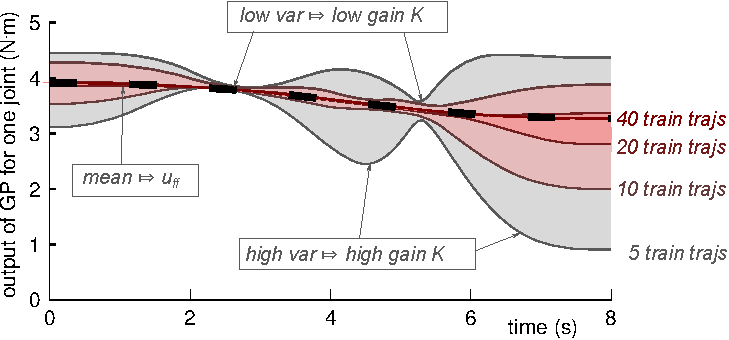
\includegraphics[width=\linewidth]{images/meanvariance.pdf}
  \caption{Mean and variance of the Gaussian process ($\mu \mp 2\sigma$) on
    the same test trajectory of 8 seconds, after having been trained with 5,
    10, 20 and 40 training trajectories. With an increasing number of training
    data, the mean of the GP approaches the true function (black dashed
    line). The known values for uff are plotted as a black dotted line.}
  \label{fig:meanvariance}
\end{figure}

%!TEX root = ../../secondYearReport.tex

% 1.68 man.months for UPMC on T4.4 

Within T4.4, UPMC studied how to deal with interferences between tasks using
machine learning tools. Whole-Body Control methods offer the potential to
execute several simultaneous tasks on highly redundant robots, such as
humanoids. Unfortunately, task combinations often result in interferences or
incompatibilities which generate undesirable behaviors. Prioritization schemes
between tasks, such as strict and soft hierarchies, are typically used to manage
these interferences but generally require a deal of time consuming and arbitrary
tuning.

To circumvent theses issues, UPMC presented a novel framework for defining and
optimizing multiple tasks in order to resolve potential interferences prior to
task execution. In a first study \cite{lober-HUMANOIDS2014} the tasks are
parameterized with Dynamical Movement Primitives, whose parameters are optimized
based on a general compatibility principle, which is independent of the robot’s
topology, tasks or environment. Two test cases on a simulation of a humanoid
robot are used to demonstrate the successful optimization of initially
interfering tasks. A video summarizing the outcome of this work can be viewed
\url{http://pages.isir.upmc.fr/~padois/website/fichiers/videos/lober_Humanoids2014.mp4}{here}.

\begin{figure}
\centering
\begin{subfigure}{.31\linewidth}
 \centering
 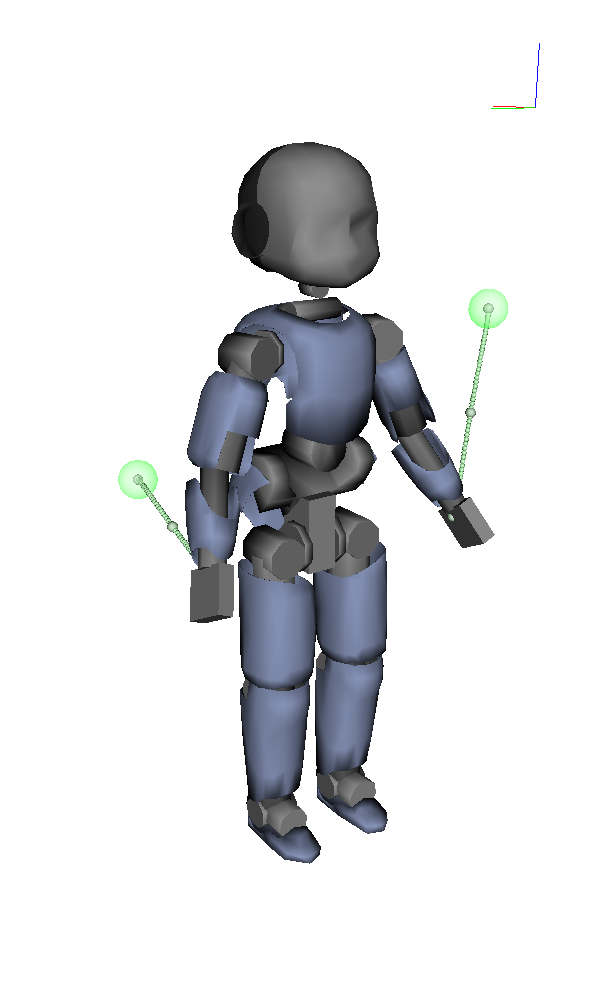
\includegraphics[trim = 0cm 4.5cm 0cm 5cm, clip, height=4 cm]{./sections/WP4/pics_UPMC/01_starting}
 \caption{Constrained Configuration}
 \label{fig:config}
\end{subfigure}
%
\begin{subfigure}{.31\linewidth}
 \centering
 \includegraphics[trim = 0cm 4.5cm 0cm 5cm, clip, height=4 cm]{./sections/WP4/pics_UPMC/02_starting}
 \caption{Workspace Violation}
 \label{fig:work}
\end{subfigure}
%
\begin{subfigure}{.31\linewidth}
 \centering
 \includegraphics[trim = 0cm 5cm 0cm 5cm, clip, height=4 cm]{./sections/WP4/pics_UPMC/03_starting}
 \caption{Balance Perturbation}
 \label{fig:balance}
\end{subfigure}
%
\caption{Three common multi-task incompatibility scenarios. The desired hand
task trajectories are indicated by the green markers. Medium size spheres
represent waypoints, and large transparent spheres represent the final waypoints
or goals.}
\label{fig:3_scenarios_lober_2015}
\end{figure}


In a second study \cite{lobersubmittedIROS2015}, UPMC studied how task
variability can be used to modulate task priorities during their execution, to
temporarily deviate certain tasks in the presence of incompatibilities. A method
for mapping from task variance to task priority was presented as well as an
approach for calculating task variance for generated trajectories. The method
successfully resolved three common task conflict scenarios online illustrated on
Fig.~\ref{fig:3_scenarios_lober_2015}.



% Refs to add to secondYearReport_WP4.bib






%Valerio's paper on learning activation policies in task controller.
TUD addressed the problem of learning the temporal profile of soft
task priorities and null-space projectors for the multi-task controllers
developed in WP3. Our preliminary results have been submitted to a robotics
conference\footnote{Modugno, V.; Neumann, G.; Rueckert, E.; Oriolo, G.; Peters,
J.; Ivaldi, S. \textit{Learning soft task prioirities and null-space projectors
for motion planning of redundant manipulators}. Submitted to IROS 2015.}.

The first controller of WP3, \textit{Prioritized Task-Space Inverse Dynamics},
is based on \textit{strict task hierarchies}, where a hierarchical ordering of
the tasks is set, such that critical tasks (or tasks that are considered as more
important) are fulfilled with higher priorities, and the low-priority tasks are
solved in the null-space of the higher priority tasks
\cite{DelPrete-2014-ID267}. The strict control approach requires the
pre-specification of the task hierarchy. However, in many contexts it is
difficult to organize the tasks in a stack and define their relative importance
in forms of priorities. When priorities are strict, a higher task can completely
block lower tasks, which can result in movements that are not satisfactory for
the robot mission (e.g., its ``global'' task). 

The second controller of WP3 is based on \textit{soft task hierarchies}, where
the solution is typically given by a combination of weighted tasks
\cite{Salini-2011-ID348}. The importance or ``soft priority'' of each individual
task is represented by a scalar weight. By tuning the vector of scalar weights,
evolving in time, the global robot behavior can be optimized. Within WP3, Liu et
al. \cite{liu_ICRA2015} propose a generalized projector (GHC) that handles
strict and non-strict priorities with smooth transitions when tasks priorities
are swapped. They show that adapting these weights may result in a seamless
transition between tasks (i.e., reaching for an object, staying close to a
resting posture and avoiding an obstacle) and in continuous task sequencing.
Despite the elegant framework, their controller needs again a lot of manual
tuning: particularly, the evolution of the tasks priorities in time, the timing
and the tasks transitions need to be designed by hand. While this approach could
still be easy for few tasks and simple robotic arms, it can quickly become
unfeasible for complex robots such as humanoids performing whole-body movements
that usually require a dozen of tasks and constraints (e.g., control balance,
posture, end-effectors, stabilize head gaze, prevent slipping, control
interaction forces etc.).

\begin{figure}%[t!]
\centering
\includegraphics[width=\linewidth]{./sections/WP4/pics_serena/concept_scheme}
\caption{This scheme briefly describes the proposed method. The control torques are computed by a combination of tasks weighted by soft priorities, represented as parameterized activation policies, that are multiplied by a Null-space projector, where some activation functions for different projectors are joined. The global task execution is evaluated and a fitness function is computed: a policy search method is then used to optimize the parameters of the activation policies, both for tasks and projector. }
\label{figure:scheme}
\end{figure}

In this task we propose a first solution to the problem of how these weights can
be learned through trial-and-error. We study how the \textit{temporal} profiles
of the task weights can be learned from a reward function, which is assumed to
be given\footnote{For many robotic task, e.g., tracking desired center-of-mass
or end-effector trajectories while avoiding obstacles, such reward functions
have been defined in \cite{Kober_IJRR_2013}.}. 

As a first step towards a controller that is capable of handling multiple tasks
and constraints on a complex robot, while allowing us to efficiently learn the
task priorities, we propose a regularized version of the Unified Framework (RUF)
proposed by Peters et al \cite{Peters_AR_2008}, where the tasks weights and
Null space projectors weights are represented by parametrized functional
approximators that can be automatically determined through a stochastic
optimization procedure. The concept is presented in Figure~\ref{figure:scheme}.

\begin{figure}%[b!]

\begin{subfigure}{.3\linewidth}
  \centering
  \includegraphics[width=\linewidth]{./sections/WP4/pics_serena/alpha1}
  \label{fig:alpha1}
  \caption{Attractor activation.}
\end{subfigure}%
\begin{subfigure}{.3\linewidth}
  \centering
  \includegraphics[width=\linewidth]{./sections/WP4/pics_serena/alpha2}
  \label{fig:alpha2}
  \caption{Null-projector activation.}
\end{subfigure}
\begin{subfigure}{.3\linewidth}
  \centering
  \includegraphics[width=\linewidth]{./sections/WP4/pics_serena/comparison}
  \label{fig:alpha3}
  \caption{Learning performance.}
\end{subfigure}
\caption{The panels in (a) and (b) show the mean and standard deviation of the temporal
profile of the activation functions $\alpha,\beta$, optimized by RUF+CMA-ES,
computed over $R=50$ replications of the same experiment of the table scenario.
(c) Comparison of our method (blue line) to the generalized projector method (GHC).}
\label{fig:activation_policy}
\end{figure}

As a first results, we show that the optimization process  generates weights
profiles that cannot be designed manually in advance, see panels (a) and (b) in 
Figure~\ref{fig:activation_policy}.

% \begin{figure}%[b!]
% \centering
% \includegraphics[width=1\hsize]{./sections/WP4/pics_serena/comparison}
% \caption{This figure shows the mean and the standard deviation of $R=20$
% replications of the same experiments for our method RUF+CMA-ES and GHC+CMA-ES.
% For both controllers, we consider a random initial point in the parameter space
% for the optimization algorithm. Our method shows a faster convergence learning
% rate and it reaches a better result in terms of the optimized fitness.}
% \label{fig:comparison}
% \end{figure}

We then compare the performance of our controller with the state-of-the-art
method GHC proposed by Liu et al. \cite{liu_ICRA2015} (WP3). We consider the
following experimental scenario: a 7-DOF KUKA Light Weight Robot arm, starting
from a vertical position, must reach a desired point with its end-effector,
while avoiding to collide with a table, represented by a surface parallel to the
z-axis in between the robot and the goal. The aim of the experiment is to bring
the end-effector as close as possible to the desired position, while avoiding
collisions with the obstacle. We define  $T=3$ tasks: a regulation task in the
joint space, and two reaching tasks for the elbow and the end-effector. For both
methods, we find the optimal profiles for the weighting functions with CMA-ES.
Our second result is that our controller generally performs better than GHC,
even if we optimize the policies in both methods: on an average of 20
replicates, our RUF+CMA-ES finds 90\% of the solutions found by our RUF+CMA-ES
satisfies the constraints, while only 75\% of the solutions of GHC+learning are
acceptable. Furthermore, the final best solution found by RUF+CMA-ES outperforms
the one of GHC+CMA-ES, as shown in Figure~\ref{fig:activation_policy} (c).


%%!TEX root = ../../secondYearReport.tex

\subparagraph{Resources}

\begin{center}
\begin{tabular}{|C{1.5cm}|C{1.5cm}|C{1.5cm}|C{2cm}|C{2cm}|C{2cm}|C{2cm}|}
\hline
\footnotesize \textbf{WP4 person months}& \footnotesize \textbf{IIT}&\footnotesize \textbf{TUD}&\footnotesize \textbf{UPMC}& \footnotesize \textbf{UB} &\footnotesize \textbf{JSI} &\footnotesize \textbf{INRIA}\\ \hline
\footnotesize Year 1 &  0.00 & 8.00 & 2.22 & 0.00 & 0.00 & -     \\  \hline
\footnotesize Year 2 &  6.04 & 21.70 & 1.68 & 2.15 & 3.00 & 2.00     \\  \hline
\footnotesize Partial &  6.04 & 29.70 & 3.90 & 2.15 & 3.00 & 2.00 \\ \hline \hline
\footnotesize Overall &  30.00 & 38.00 & 9.00 & 12.00 & 10.00 & 9.00 \\ \hline
\end{tabular}
\end{center}

\subparagraph{Deviations from workplan} 
Six person months of UPMC planned for Serena Ivaldi were transfered to TUD. No significant deviations. 


%!TEX root = ../../secondYearReport.tex

\paragraph{Work package 5 progress}

The activities in WP5 are divided into four tasks corresponding to the four years project duration. As a result, during the second year CoDyCo results concentrate on T5.2. The main result consist in the implementation of the validation scenario consisting of the balancing on different type of rigid contacts.

\subparagraph{Scenario 2: iCub posture control while performing goal directed actions (T5.2)}

The main contributions to T5.2 have been presented in ``Validation scenario2: balancing on feet while performing goal directed actions.'' which discusses the technical implementation of the second year validation scenario (see \url{https://github.com/robotology-playground/codyco-deliverables/tree/master/D5.2/pdf}). The software developed for the scenario implementation is released with an open-source license and distributed through github (\url{https://github.com/robotology/codyco-modules} ). The main software activities include: a module to identify the whole-body motor transfer functions (\url{https://github.com/robotology/codyco-modules/tree/master/src/modules/motorFrictionIdentification}), a module for estimating whole-body internal (joint torques) and external (contact) forces (\url{https://github.com/robotology/codyco-modules/tree/master/src/modules/wholeBodyDynamicsTree}), a module for whole-body joint torque control (\url{https://github.com/robotology/codyco-modules/tree/master/src/devices/jointTorqueControl}), a C++ module for whole-body control under multiple rigid contacts (\url{https://github.com/robotology/codyco-modules/tree/master/src/modules/torqueBalancing}).



%\begin{itemize}
%\item[-] \emph{\color{red}[A summary of progress towards objectives and details for each task;]}
%\item[-] \emph{\color{red}[Highlight clearly significant results;]}
%\item[-] \emph{\color{red}[If applicable, explain the reasons for deviations from Annex I and their impact on other tasks as well as on available resources and planning;]}
%\item[-] \emph{\color{red}[If applicable, explain the reasons for failing to achieve critical objectives and/or not being on schedule and explain the impact on other tasks as well as on available resources and planning (the explanations should be consistent with the declaration by the project coordinator) ;]}
%\item[-] \emph{\color{red}[a statement on the use of resources, in particular highlighting and explaining deviations between actual and planned  person-months per work package and per beneficiary in Annex 1 (Description of Work);]}
%\item[-] \emph{\color{red}[If applicable, propose corrective actions.]}
%\end{itemize}

%%!TEX root = ../../secondYearReport.tex

\subparagraph{Resources}

Resources were used with small difference with respect to what planned. In particular IIT invested only 2 PM with respect to 12PM planned. The motivation resides in the fact that WP5 took advantage of the significant effort done in WP1 (software) and WP3 (control) and in a sense resources initially planned on T5.1 eventually have been committed to T1.1, T1.2, T1.3, T3.1 and T3.2.

\begin{center}
\begin{tabular}{|C{1.5cm}|C{1.5cm}|C{1.5cm}|C{2cm}|C{2cm}|C{2cm}|C{2cm}|}
\hline
\footnotesize \textbf{WP5 person months}& \footnotesize \textbf{IIT}&\footnotesize \textbf{TUD}&\footnotesize \textbf{UPMC}& \footnotesize \textbf{UB} &\footnotesize \textbf{JSI} & \footnotesize \textbf{INRIA} \\ \hline
\footnotesize Year 1 &  2.00 & 0.00 & 0.31 & 0.00 & 0.00 & 0.00     \\  \hline
\footnotesize Year 2 &  12.00 & 0.85 & 0.05 & 0.00 & 0.00 & 0.00     \\  \hline
\footnotesize Partial &  14.00 & 0.85 & 0.36 & 0.00 & 0.00 & 1.50 \\ \hline \hline
\footnotesize Overall &  48.00 & 5.00 & 2.50 & 0.00 & 0.00 & 1.50 \\ \hline
\end{tabular}
\end{center}

\subparagraph{Deviations from workplan} 
The original work plan was leaving quite a flexible set of possibilities for both the postural task (e.g. sitting on a chair or balancing on the feet) and the goal oriented action (e.g. opening a drawer while standing or manipulating object while sitting). In the final validation scenario it was chosen to consider a interactive scenario, with the torque controlled iCub standing on his feet while trying to grasp an object moved by the experimenter. As soon as the object exceeds the robot workspace, the iCub takes a forward step in order to increase his workspace. 

UPMC covered the activities within WP5 with own resources for a total of 0.45 PM. In particular Ryan Lober (PhD student, French PhD research grant) and Darwin Lau (Postdoctoral scholar) participated to the deployment of the whole-body interface developed in WP1 on the iCub robots present at UPMC.


%!TEX root = ../../secondYearReport.tex


\paragraph{Work package 6 progress}

Activities within work package 6 achieved the expected results both in terms of administrative activities and management activities. As a major achievement, the management successfully concluded a second amendment to include INRIA as a partner. The inclusion was motivated by the the new position of Dr. Serena Ivaldi, currently researcher at INRIA, Nancy. 

\subparagraph{Administrative coordination (T6.1)}
Administration was successfully coordinated by IIT, with significant contribution from Chiara Andreoli (iCub Facility), Francesca Boscolo (project offices) and Maria Carmela Fierro (Robotics, Brain and Cognitive Science Department). The major activity concerned the amendment that the CoDyCo consortium asked the main reason being the fact that Serena Ivaldi, initially hired by UPMC and successively moved to TUD, was recently hired by INRIA as researcher. Part of the administrative coordination activities were also conducted during the mid-year meeting: November 20th-21st, 2014, Ljubljana.  Details on the meetings can be found in the CoDyCo website (\url{http://www.codyco.eu}).

\subparagraph{Software repository implementation (T6.2)}

The github software repository was several times restructured \url{https://github.com/robotology/codyco} and the contribution from the different developers can be directly checked in the website. 
%%!TEX root = ../../secondYearReport.tex


\subparagraph{Resources}

Resources were used as follows.

\begin{center}
\begin{tabular}{|C{1.5cm}|C{1.5cm}|C{1.5cm}|C{2cm}|C{2cm}|C{2cm}|C{2cm}|}
\hline
\footnotesize \textbf{WP6 person months}& \footnotesize \textbf{IIT}&\footnotesize \textbf{TUD}&\footnotesize \textbf{UPMC}& \footnotesize \textbf{UB} &\footnotesize \textbf{JSI} & \footnotesize \textbf{INRIA} \\ \hline
\footnotesize Year 1 &  1.46 & 0.00 & 0.25 & 0.00 & 0.10 & 0.00    \\  \hline
\footnotesize Year 2 &  1.50 & 0.00 & 0.31 & 0.00 & 0.00 & 0.00     \\  \hline
\footnotesize Partial &  2.96 & 0.00 & 0.56 & 0.00 & 0.10 & 0.00 \\ \hline \hline
\footnotesize Overall &  5.00 & 1.00 & 1.00 & 0.60 & 1.00 & 0.00 \\ \hline
\end{tabular}
\end{center}

\subparagraph{Deviations from workplan} 
No significant deviations. 

%!TEX root = ../../secondYearReport.tex


\paragraph{Work package 7 progress}

Dissemination and exploitation activities included the participation to international events addressed to both commercial and academic institutions. 

\subparagraph{Dissemination activities towards academia, industry, and other users (T7.1)}

Dissemination activities were conducted thorough international publications, organisation of international events, talks at international conferences, press interviews and iCub expositions at international events. Here is the overall contribution subdivided by partner:

\begin{itemize}

\item IIT: 4 invited talks, 4 organised international events, 6 talks at international conferences, 10 publications (2 journal, 7 internal conferences, 1 book chapter), 10 media coverage events.

\item TUD: 15 invited talks, 4 organised international events, 7 publications (7 internal conferences), 7 media coverage events.

\item UPMC: 3 invited talks, 6 publications (6 internal conferences), 1 media coverage event.

\item UB: 3 invited talks, 5 publications (5 internal conferences), 5 talks at international conferences.

\item JSI: 1 invited talks, 1 organised special issue, 2 talks at international conferences, 7 publications (1 journal, 6 internal conferences).

\item INRIA: 4 invited talks, 4 organised international events, 8 publications (4 journal, 4 internal conferences), 3 media coverage events

\end{itemize}

Live demonstration of the iCub have been performed at several international events.  Some of these events were sponsored by CoDyCo and the following is a non exhaustive list:

\begin{enumerate}

\item 12$^{th}$-14$^{th}$ March 2014. EU Robotics Forum Rovereto. \url{http://www.erf2014.eu/erf_home.jsp}.
\item 3$^{rd}$-6$^{th}$ June 2014. Automatica 2014, Munich, Germany. \url{http://www.nfm-automatica.de/2014/en/home.php}.
\item 3$^{rd}$-5$^{th}$ October 2014. European Maker Faire, Roma, Italy. \url{http://www.makerfairerome.eu/en/agenda2014/}. 
\item 18$^{th}$-20$^{th}$ November 2014. 2014 IEEE-RAS International Conference on Humanoid Robots (Humanoids 2014), Madrid, Spain. \url{http://www.humanoids2014.com}.

\end{enumerate} 

Among the invitations as a speaker at international events it is worth citing the following:

\begin{enumerate}

\item Francesco Nori: invited speaker at the Journ�es Nationales du GdR Robotique 2014, held at Grand amphith\'e\^atre du Centre Arts et M\`etiers ParisTech, 151-155 boulevard de l'H�pital, 75013 Paris. 30 October 2014. \url{http://www.gdr-rob2014.org}.

\item Serena Ivaldi: invited speaker French-German-Japan Workshop on Humanoid and Legged robots. Social learning and engagement in human-humanoid interactions. \url{http://orb.iwr.uni-heidelberg.de/hlr2014/HLR14}.

\item Jan Babic: invited talk in Paris at the Universit� Pierre et Marie Curie. Synthesis of skilled robotic behaviour through human sensorimotor adaptation:  12$^th$ November 2014.

\item Jan Peters: keynote for the Learning by Demonstration Session Topic at the IEEE/RSJ International Conference on Intelligent Robots and Systems (IROS), Chicago, USA.

\item Jan Peters: invited plenary talk speaker at the 13th International Conference on Intelligent Autonomous Systems (IAS-13), Padua, Italy.

\item Vincent Padois: invited talk at the Cap Digital/Innorobo day about Robotics et Innovations. ``Issues and challenges of interactive robotics in complex industrial contexts''. Lyon, France - March 2014.

\item Michael Mistry: invited Lecturer at European Computational Motor Control Summer School. June 15$^th$-21$^st$, 2014.

\end{enumerate} 

Among the organised international events here is a non exhaustive list of the most relevant events:

\begin{enumerate}

\item IIT: workshop organisation at the 2014 IEEE-RAS international conference on humanoid robots (Humanoids 2014). ?One day with a humanoid robot: a crash course on the iCub software tools?. Coordinators: L. Natale, F.Nori, U. Pattacini, V. Tikhanoff, M. Randazzo, G. Metta (Italy).

\item IIT: iCub summer school (Veni Vidi Vici 2014). In 2014, the school was held in Sestri Levante, Italy, July 21-30 2014. Main organisers: Giorgio Metta, Lorenzo Natale, Francesco  Nori, Vadim Tikhanoff, Ugo Pattacini.

\item INRIA, TUD, UB, JSI: editors for the Autonomous Robots special Issue: ``Whole-body control of contacts and dynamics for humanoid robots''. 

\end{enumerate} 



\subparagraph{Exploitation plan (T7.2)}

The second year activities on T7.1 and T7.2 are all contained in ``D7.1 Dissemination and exploitation plan'' available here: \url{https://github.com/robotology-playground/codyco-deliverables/tree/master/D7.1/pdf}.

\subparagraph{Management of IPR (T7.3)}

No activities to be reported during the second year on this task in consideration of the fact that the task started at the very end of the second year. As a minor starting activity the consortium circulated a list containing each partner responsible contact person for the IPR management. This list is contained in ``D7.1 Dissemination and exploitation plan'' available here: \url{https://github.com/robotology-playground/codyco-deliverables/tree/master/D7.1/pdf}.

\subparagraph{Dissemination of a database of human motion with contacts (T7.4)}

During the second year of CoDyCo, IIT completed the task of setting up a database for storing both human and robot datasets. The details on the database are reported in ``D7.2 Standard database with support materials'' available here \url{https://github.com/robotology-playground/codyco-deliverables/tree/master/D7.2/pdf}. 


%%!TEX root = ../../secondYearReport.tex


\subparagraph{Resources}

Resources were used as follows.

\begin{center}
\begin{tabular}{|C{1.5cm}|C{1.5cm}|C{1.5cm}|C{2cm}|C{2cm}|C{2cm}|C{2cm}|}
\hline
\footnotesize \textbf{WP7 person months}& \footnotesize \textbf{IIT}&\footnotesize \textbf{TUD}&\footnotesize \textbf{UPMC}& \footnotesize \textbf{UB} &\footnotesize \textbf{JSI} & \footnotesize \textbf{INRIA} \\ \hline
\footnotesize Year 1 &  1.00 & 0.00 & 0.40 & 0.00 & 0.00 & - \\  \hline
\footnotesize Year 2 &  0.00 & 0.00 & 0.13 & 0.00 & 0.00 & 1.00 \\  \hline
\footnotesize Partial & 1.00 & 0.00 & 0.53 & 0.00 & 0.00 & 1.00 \\ \hline \hline
\footnotesize Overall & 3.00 & 1.00 & 1.00 & 1.00 & 1.00 & 1.00 \\ \hline
\end{tabular}
\end{center}

\subparagraph{Deviations from workplan} 
No significant deviations. 

\bibliography{ias_bibliography,ias_state_of_art}
\bibliographystyle{plain}

\end{document}
\endinput
%%
%% End of file `elsarticle-template-num.tex'.
